%%%%%%%%%%%%%%%%%%%% book.tex %%%%%%%%%%%%%%%%%%%%%%%%%%%%%
%
% sample root file for the chapters of your "monograph"
%
% Use this file as a template for your own input.
%
%%%%%%%%%%%%%%%% Springer-Verlag %%%%%%%%%%%%%%%%%%%%%%%%%%


% RECOMMENDED %%%%%%%%%%%%%%%%%%%%%%%%%%%%%%%%%%%%%%%%%%%%%%%%%%%
\documentclass[graybox,envcountchap,sectrefs,fleqn]{svmono}
\usepackage{listings}
% \lstset{numbers=left, numberstyle=\small, numbersep=8pt, frame = single, language=R, framexleftmargin=15pt}
% \lstset{
% numbers=left, 
% numberstyle=\small, 
% numbersep=8pt, 
% frame = single, 
% language=R, 
% framexleftmargin=15pt}
\usepackage{minibox}
\usepackage{nameref}
\usepackage{color}
\usepackage[dvipsnames,svgnames,table]{xcolor}
 \usepackage{appendix}
\definecolor{codegreen}{rgb}{0,0.6,0}
\definecolor{codegray}{rgb}{0.5,0.5,0.5}
\definecolor{codepurple}{rgb}{0.58,0,0.82}
\definecolor{backcolour}{rgb}{0.95,0.95,0.92}
 
\lstdefinestyle{mystyle}{
    backgroundcolor=\color{backcolour},   
    commentstyle=\color{codegreen},
    keywordstyle=\color{magenta},
    numberstyle=\tiny\color{codegray},
    stringstyle=\color{codepurple},
    basicstyle=\footnotesize,
    breakatwhitespace=false,         
    breaklines=true,                 
    captionpos=b,                    
    keepspaces=true,                 
    numbers=left,                    
    numbersep=5pt,                  
    showspaces=false,                
    showstringspaces=false,
    showtabs=false,                  
    tabsize=2
}
 
\lstset{style=mystyle,language=R}
\usepackage{rotating}
\usepackage{array}
\usepackage{geometry}
 \geometry{
 a4paper,
 total={210mm,297mm},
 left=25mm,
 right=20mm,
 top=25mm,
 bottom=25mm,
 }
% choose options for [] as required from the list
% \usepackage{setspace}
% in the Reference Guide
\usepackage{amsmath,amssymb, amstext, bm}
\usepackage{manyeqns}
\usepackage{ragged2e}
% \usepackage{amssymb}
%  \usepackage[fleqn]{amsmath}
\usepackage{mathptmx}
\usepackage{helvet}
\usepackage{courier}
%
\usepackage{xcolor}
\usepackage{hyperref}
%\hypersetup{colorlinks=false,linkbordercolor=red,linkcolor=green,pdfborderstyle={/S/U/W 1}}
% \hypersetup{%
%   colorlinks=true,% hyperlinks will be coloured
%   linkcolor=red,% hyperlink text will be green
%   linkbordercolor=red,% hyperlink border will be red
% }
\hypersetup{urlcolor=magenta, colorlinks=true, linkcolor=magenta, citecolor=blue, menucolor=magenta]}
% \usepackage{cite}
% \renewcommand{\citeleft}{\textcolor{red}{[}}
% \renewcommand{\citeright}{\textcolor{red}{]}}

\usepackage{type1cm}         

\usepackage{makeidx}         % allows index generation
\usepackage{graphicx}        % standard LaTeX graphics tool
                             % when including figure files
\usepackage{multicol}        % used for the two-column index
\usepackage[bottom]{footmisc}% places footnotes at page bottom
% \usepackage[square, numbers, comma, sort&compress]{natbib} 
\usepackage{natbib}
\usepackage{chapterbib}
\usepackage{tikz}
\usepackage{suffix}
\usepackage{enumitem}
\usepackage{changepage}
\newcommand\chapterauthor[1]{\authortoc{#1}\printchapterauthor{#1}}
\WithSuffix\newcommand\chapterauthor*[1]{\printchapterauthor{#1}}
% \singlespacing
\makeatletter
\newcommand{\printchapterauthor}[1]{%
  {\parindent0pt\vspace*{-25pt}%
  \linespread{1.1}\large\scshape#1%
  \par\nobreak\vspace*{35pt}}
  \@afterheading%
}
\newcommand{\authortoc}[1]{%
  \addtocontents{toc}{\vskip-10pt}%
  \addtocontents{toc}{%
    \protect\contentsline{chapter}%
    {\hskip1.3em\mdseries\scshape\protect\scriptsize#1}{}{}}
  \addtocontents{toc}{\vskip5pt}%
}
\makeatother
\graphicspath{{Figures/}}
% see the list of further useful packages
% in the Reference Guide

\usepackage{titlesec}

\setcounter{secnumdepth}{4}

\titleformat{\paragraph}
{\normalfont\normalsize\bfseries}{\theparagraph}{1em}{}
\titlespacing*{\paragraph}
{0pt}{3.25ex plus 1ex minus .2ex}{1.5ex plus .2ex}


\makeindex             % used for the subject index
                       % please use the style svind.ist with
                       % your makeindex program

%%%%%%%%%%%%%%%%%%%%%%%%%%%%%%%%%%%%%%%%%%%%%%%%%%%%%%%%%%%%%%%%%%%%%
\setlength\parindent{0pt}
\setlength{\mathindent}{10pt}
% \setlength{\parskip}{\baselineskip}


\usepackage{rotating}
\usepackage{booktabs}
\newcolumntype{P}[2]{%
  >{\begin{turn}{#1}\begin{minipage}{#2}\small\raggedright\hspace{0pt}}l%
  <{\end{minipage}\end{turn}}%
}

% \usepackage{array}
\newcommand{\spheading}[2][10em]{% \spheading[<width>]{<stuff>}
  \rotatebox{90}{\parbox{#1}{\raggedright #2}}}

  \usepackage{subcaption}
\usepackage[section]{placeins}

\begin{document}

\author{Bryan T. Adey and Nam Lethanh}
\title{Infrastructure Maintenance Processes}
\subtitle{Lecture notes}
\maketitle

\frontmatter%%%%%%%%%%%%%%%%%%%%%%%%%%%%%%%%%%%%%%%%%%%%%%%%%%%%%%
%%%%%%%%%%%%%%%%%%%%%%foreword.tex%%%%%%%%%%%%%%%%%%%%%%%%%%%%%%%%%
\foreword
This document has been compiled to provide students taking the above mentioned course in understanding the examples given in class and assignments. All questions presented have been prepared by the authors based to varying degrees on different sources. The sources are given for each example.

This document is being issued so that students taking the course may better prepare for the exam. As it has not yet undergone the complete rigorous control processes of IBI this document is to be considered a work in progress and is hence labeled as a DRAFT.


\vspace{\baselineskip}
\begin{flushright}\noindent
IBI-ETH, September 2015\hfill {\it Professor: Bryan T. Adey}\\
\hfill {\it Dr: Nam Lethanh}\\
\end{flushright}



%\include{./General/preface}


\tableofcontents

%\include{acronym}


\mainmatter%%%%%%%%%%%%%%%%%%%%%%%%%%%%%%%%%%%%%%%%%%%%%%%%%%%%%%%
\setlength{\parskip}{\baselineskip}

\include{./Chapters/part}
\include{./Chapters/introduction}
%%%%%%%%%%%%%%%%%%%%% chapter2.tex %%%%%%%%%%%%%%%%%%%%%%%%%%%%%%%%%
%
% sample chapter
%
% Use this file as a template for your own input.
%
%\motto{Use the template \emph{chapter.tex} to style the various elements of your chapter content.}
\chapter{Level of Service - Impact Hierarchy}
\label{2:los} % Always give a unique label
% use \chaptermark{}
% to alter or adjust the chapter heading in the running head
\chapterauthor{Bryan T. Adey and Nam Lethanh}
\section{General}
In order to determine what to do with infrastructure it is necessary to determine what is expected from the infrastructure, i.e. it is necessary to determine the required LOSs. This must be defined for a specific time period. It requires the determination of an impact hierarchy and the determination of the values of each impact indicator or impact value over the specified period of time \citep{Adey2012}.
\section{Impact hierarchy - Theory}
\subsection{General}
The best way to define LOS provided by infrastructure is to consider it to be identical to the amount that persons are affected by the functioning (or non-functioning) of infrastructure with respect to the required LOS. For example, on a road network, it may be expected that next year $x$ $mus$\footnote{$mus$ stands for monetary units} are to be spent on the execution of maintenance interventions and y mus worth of impacts are due to accidents. If more than $x$ $mus$ are to be spent on maintenance and more than $y$ $mus$ worth of impacts occur due to accidents than it can be considered that an inadequate LOS was provided. If less or equal, than it can be considered that an adequate LOS was provided.

If it is too difficult to quantify all impacts to be used to measure LOS in terms of directly comparable units (above they are given in $mus$) proxies can be used. For example, instead of stating that y mus worth of impacts due accidents are expected next year, the number of accidents may be stated. 

The type of proxy used can be evaluated with respect to its usefulness in assessing the amount that persons are affected by the functioning (or non-functioning) of infrastructure with respect to the required LOS. For example, the number of accidents might be considered a relatively good proxy with respect to the amount persons are affected by accidents, whereas the number of potholes in the road, might not be. The number of accidents can be multiplied by the average impact of an accident to give the expected total impacts, whereas if the number of potholes is used to calculate the expected total impact, it must be multiplied with the expected number of accidents that occur when there are this number of and the average impact of an accident \footnote{the expected number of accidents when a road section has $x$ numbers of potholes is often estimated as probabilistic function that takes into account of some factors such as numbers of potholes, traffic volume, vehicle speed, etc.}. In general, the fewer the number of calculations that are required to determine the amount that persons are affected, the better.

In any case, the determination of the values of the proxies to be used should be approximated based on a rigorous assessment of the impacts related to these values, and a comparison of these values with the other impact types used to define LOS. If not, an optimal performance of the infrastructure will not be targeted.

It is important to define the LOS so that it covers all ways in which persons can be affected by the functioning (or non-functioning) of infrastructure. If this is not done, then there is a significant probability that managers will concentrate on some impacts and ignore others, which may also be important. For example, a manager might choose to reduce the probability of occurrence of an accident in a tunnel to a very small amount by imposing a regulation to reduce vehicle speed (e.g. from 100 km/hour to 80 km/hour) in the tunnel if only owner costs and accident costs are considered. If, however, owner costs, the costs of travel time and the costs of accidents are taken into consideration he may determine that the best strategy is to renew the road surface and the lighting system more frequently, even though it would result in higher costs for the owner.

To ensure that all this can be done it is useful to:

\begin{itemize}%[leftmargin=2pt-.8in]
\item determine the objective of setting the LOS
\item determine and classify the persons affected by the functioning (or non-functioning) of the infrastructure, i.e. stakeholders
\item determine and classify the ways in which each of the stakeholders are affected, i.e. the impact types. 
\item determine the indicators to be used to determine the value of the impacts incurred by stakeholders,
\item determine the value of a unit change in the indicators used in units that can be compared across all impact types.                                                                                                                    \end{itemize}


The grouping of stakeholders, their impacts at each level, and the indicators to be used to measure these impacts are referred to as an impact hierarchy. In the development of an impact hierarchy it is important that it is: 

\begin{enumerate}
\item \textbf{complete} - all non-negligible ways in which persons are affected should be included. If not, there will be an unwanted focus on the items included in the hierarchy to the detriment of those that are not, which may lead overall to sub-optimal decisions.
\item \textbf{decomposable} - each impact should be broken down, or decomposed, to a level that is reasonable quantifiable. If the hierarchy is not decomposable to a reasonable good quantifiable level persons will be required to place numbers on impacts relatively subjectively.  
\item \textbf{operational} - the impacts should be defined in a way and a level which it is reasonable to quantify them in terms of effort. If a hierarchy is defined in too much detail the effort will be too large to conduct the required analysis or to collect the required information. If a hierarchy is defined in too little detail, there will be so much subjectivity in the assessment of the value of the impacts that the results will be relatively useless. 
\item \textbf{non-redundant, or orthogonal} - the impacts should be defined in a way that ensures impacts are not double counted. To help ensure orthogonality it is sometimes helpful to make use of the pillars of sustainability, i.e. economic, environmental, and social, in the definition of the lowest level impacts in the hierarchy. If the hierarchy is not orthogonal than the double counting of some, but not all, of the impacts will result in overall sub-optimal decisions.                                                                                                                                                                                                                                                                                                                                                                                                                                                                                 \end{enumerate}
%
\subsection{Objective}
The stakeholders, impacts types and proxies to be considered depend on the objective of determining the LOS. For example, if a road manager wants to determine the work program that will maximize the net positive impact that society as a whole obtains from the infrastructure, only changes that are relevant to society as a whole are considered, and therefore positive impacts on one stakeholder that are negative impacts on another are not taken into consideration. For example, the income that is received from charging a toll on a public road would not be considered as it is a positive impact on the owner but a negative impact of equal magnitude on the user.
%
\subsection{Stakeholder}
There are many ways to classify these persons. It is, however, advantageous to group them keeping in mind how models will be built to assess how they are affected over time. For example, a person affected by noise who is driving a car may not be affected in the same way as a person who lives next to road on which cars pass.

Being a stakeholder is time dependent. For example, when a person is driving a vehicle on a road he is a user at that point in time, but when he is off of the road and in his house far from the road he is part of the indirectly affected public. Although he is the same person he is affected by the road when he is using it in one way, and when he is not using it in another way.

Depending on the objective it can be helpful to classify stakeholders as either first level, or second level or third level stakeholders. The first level stakeholders are those whose net positive impacts should be maximized. The second level stakeholders are those whose impacts are the outcome of the maximization of the net impacts of the first level stakeholders, and should be monitored.  The third level of stakeholders are those whose impacts are of no concern.
%
\subsection{Impact}
Each stakeholder can be affected by the functioning (or non-functioning) of the infrastructure in different ways. For example, someone driving on a road can be affected by being in an accident or through the amount of time they spend traveling. 

The impacts are attributed to the stakeholder who is most directly affected. For example, the money spent to hire persons to execute an intervention on a bridge should be attributed to the owner of the bridge rather than the tax payers.

The impact are to be grouped in a hierarchy and given to a level of detail in a way in which it can be reasonably expected that they can be quantified. 

The impact hierarchy should include all non-negligible impacts to the “principal” stakeholders of public road infrastructure, i.e. those whose positive impacts should be maximized. 

\subsection{Indicator}
In order to estimate the impacts it is necessary to determine impact indicators, which are considered to be representative of each impact type. It is only by estimating the values of these indicators over time, and attributing monetary values to each unit change in the indicators, that the impact on the stakeholders can be correctly evaluated. If the values of these indicators are used directly to set a LOS they are referred to as proxies.

\subsection{Conclusions}
Determination of the impact hierarchy is the precursor to setting the required LOS. It is important that sufficient time be spent to define it well, and to ensure that decision makers understand it. It is only with this understanding that the statement of the required LOS will make sense, which will set the stage for good decision making in the future.

Ideally the determination of the required LOS would be closely linked to the theoretically optimal LOS, i.e. the stakeholders as a whole receive the maximum net benefit from the infrastructure. As there are, however, many different stakeholders affected by the functioning (or non-functioning) of infrastructure, with many different opinions of the values to be associated with the unit changes in different types of impacts, the fixing of the required LOS is something that is associated with considerable negotiation between all involved stakeholders \citep{Brauers204}.

\section{Impact hierarchy - an example}
\subsection{Question A}

Develop an impact hierarchy that will allow a public road manager to determine the work program that will maximize the net positive impact that society as a whole obtains from the infrastructure over the next 20 years. Be clear as to the objective of developing the impact hierarchy. Explain the main components of the hierarchy in general. Give the complete hierarchy. Explain how you would attempt to quantify each impact type at the lowest level. 

\subsection{Answer A}

\label{GrindEQpgref4d79f6d52}\subsubsection{Objective}

This impact hierarchy is developed for public roads assuming that a road manager wants to determine the work program that will maximize the net positive impact that society as a whole obtains from the infrastructure Therefore, only changes that are relevant to society as a whole are considered, i.e. positive impacts on one stakeholder that are negative impacts on another are not taken into consideration. For example, the income that is received from charging a toll on public road is not considered as it is a positive impact on the owner but a negative impact of equal magnitude on the user.

\subsubsection{Components}

The impact hierarchy is to consist of stakeholders, impact types and impact indicators.


\paragraph{\underline{Stakeholders}}

A stakeholder is considered as an individual, group, or organization, which is affected by changes to public roads. Being a stakeholder is time dependent, i.e. when a person is driving a vehicle on a road he is a user at that point in time. When he is off of the road and in his house far from the road he is part of the indirectly affected public. It is considered that all stakeholders can be grouped as either first level or second level stakeholders. The first level stakeholders are those whose net positive impacts should be maximized. The second level stakeholders are those whose impacts are the outcome of the maximization of the net impacts of the first level stakeholders, and should be monitored. 

The four first level stakeholder groups are the owner, the user, the directly affected public (DAP), and the indirectly affected public (IAP). It is assumed that all impacts to be maximized can be attributed to one of these four stakeholder groups. The impacts are attributed to the stakeholder who is most directly affected. The definitions of each stakeholder group are given in later parts of this section. 

The proposed impact hierarchy is to be used to take into consideration all non-negligible impacts to the ``principal'' stakeholders of public road infrastructure, i.e. those whose positive impacts should be maximized. It is considered that all people at a point in time can be divided into one of four stakeholder groups, the owner, the user, the directly affected public, and the indirectly affected public. The impact types in the hierarchy are given to a level of detail in which they could be reasonably expected to be quantified. To help ensure orthogonality the pillar of sustainability, i.e. economic, environmental, social, is stated for each of the lowest level impacts. An example of each impact type is given.

\begin{table}[htbp]
\caption{Stakeholders}
\begin{tabular}{|p{90pt}|p{170pt}|p{170pt}|}
\hline
Stakeholders & Definition & Examples \\ \hline
Owner & the persons who are responsible for decisions with respect to physically modifying the infrastructure & a federal road authority  \\ \hline
Users & the persons who are using the roads & a driver and passengers of a vehicle on a road. \\ \hline
Directly affected public & the persons who are in the vicinity of the road but are not using it & persons in a house next to the road that hear vehicles driving on the road. \\ \hline
Indirectly affected public & the persons who are not in the vicinity of the road but are affected by its use & persons in a house far away from the road that do not hear vehicles driving on the road, but are affected by a changing climate due to the emissions produced by vehicles driving on the road. \\ \hline
\end{tabular}
\label{tbl:21}
\end{table}

Second level stakeholder groups, such as contractors, financial institutions, and operators are not considered further than they are considered when considered as one of the above listed stakeholders. The impacts on these stakeholder groups are only the outcome of our efforts to maximize the positive net impact of the four first level stakeholders in the first level.

\paragraph{\underline{Impact types}}

The impacts on each stakeholder are grouped as impact types. The impact types are subdivided at increasingly fine levels until the impact of each type can be reasonably and objectively quantified and modelled. To help to ensure orthogonality in the impact hierarchy, each impact type, on the lowest defined level, is explained and classified as contributing to one of the pillars of sustainability (economic, societal, environmental). An example is given for each to help clarify its meaning. 

\paragraph{\underline{Impact indicators}}

Impact indicators, which are considered to be representative of each impact type are given for each impact type. By estimating the values of these indicators over time, and attributing monetary values to each unit change in the indicators, it is possible to evaluate the impact of the stakeholders. Examples of models to be used to estimate how their values change over time per impact type are given in section 5. The impact hierarchy is given in Table \ref{tbl:22} to Table 5 in the following sections.

\subsubsection{Impact hierarchy}

\paragraph{\underline{Owner}}

The impacts attributed to the owner are grouped as intervention costs (Table \ref{tbl:22}), i.e. the impact on the owner of executing interventions. The impact indicators are the amount of labour, the amount of equipment, and the amount of material to be used to execute interventions, $I_{labor}^o$\textit{,,}$I_{material}^o$ e.g. intervention \textit{w} required \textit{x} man-hours, \textit{y} generator-hours and \textit{z} kilograms of material\footnote{Throughout the document, I represents ``impact'' and it is used to as mathematical notation in functions where appropriate.}. 

The monetary value placed on the 

\begin{itemize}
	\item labor used represents the economic impact of persons performing tasks, i.e. the value from society's perspective of the person doing the intervention. 
	\item material used represents the economic impact of people ensuring that materials are available for use, i.e. the value from society's perspective of persons preparing the materials for use. 
	\item equipment used represents the economic impact of people ensuring that equipment is available for use, i.e. the value from society's perspective of persons preparing the equipment for use.
\end{itemize}

The estimation of the value of an intervention is often done using one of two approaches:

\begin{itemize}
	\item a disaggregate approach where expenditures for each item or activity are estimated and summed. When this approach is used the work break down structure of the intervention project it is often used.
	\item an aggregate approach where sum of all expenditures is estimated directly. An aggregate approach often includes regression analysis and historical information. 
\end{itemize}

\begin{table}[htbp]
\caption{Owner impact types}
\begin{tabular}{|l|p{100pt}|p{70pt}|p{170pt}|}
\hline
\multicolumn{2}{|l|}{Level 1} & \multicolumn{2}{l|}{Level 2} \\ 
\hline
Label & Description & Label & Description \\ 
\hline
Intervention & the impact of executing interventions & Labor* & the economic impact of people performing tasks \\ 
\cline{3-4}
 &  & Material* & the economic impact of people ensuring that materials are available for use \\ 
\cline{3-4}
 &  & Equipment* & the economic impact of people ensuring that equipment is available for use \\ 
\hline
\end{tabular}\\
\label{tbl:22}
\footnotesize * These could be further subdivided based on the type of activity performed, e.g. administration, planning, etc...
\end{table}


\paragraph{\underline{User}}

During the interventions, users experience inconveniences such as traffic jams, bumping condition of temporarily roads (detour roads). The unfavorable conditions of traveling via the road sections and links subjected to intervention will eventually lead to higher possibility of accidents, various types of physical exhaustion and illness as comfort levels decrease, loss of travel time, and increases in fuel consumption and frequency of the maintenance of vehicles.

In between interventions, deterioration processes result in a worsening condition of any infrastructure object. The increasingly poor condition of infrastructure also results in a change in how stakeholders are affected e.g. increases in the number of accidents, travel time, the costs of operating and maintaining vehicles.

The impacts attributed to the user are grouped as: safety, operation efficiency, operation quality, and environment preservation (Table \ref{tbl:23}). 

\begin{table}[htbp]
\caption{User impact types}
\begin{tabular}{|p{70pt}|p{100pt}|p{70pt}|p{150pt}|}
\hline
\multicolumn{2}{|l|}{Level 1} & \multicolumn{2}{l|}{Level 2} \\ 
\hline
Label & Description & Label & Description \\ 
\hline
Safety & the impact on the user due to the user being involved in an accident & property damage & the economic impact of repairing the vehicle \\ 
\cline{3-4}
 &  & injury & the societal impact due to the injury \\ 
\cline{3-4}
 &  & death & the societal impact due to death \\ 
\hline
Operation efficiency & the impact of travel in terms of time required & work & the economic impact of wasting work time traveling \\ 
\cline{3-4}
 &  & leisure & the economic impact of wasting leisure time traveling \\ 
\cline{2-4}
 & the impact of travel in terms of vehicle costs & operation & the economic impact of people ensuring that fuel and oil is available for use \\ 
\cline{3-4}
 &  & maintenance & the economic impact of people repairing vehicles and ensuring that materials, e.g. tires and brake pads, are available for use \\ 
\hline
Operation quality & the impact of traveling on the user & physical & the societal impact of obtaining for example, bruises from an extremely bumpy ride \\ 
\cline{3-4}
 &  & psychological & the societal impact of having for example, anxiety due to a perceived increase in the probability of being involved in an accident, or of seeing things while traveling. \\ 
\hline
Environment preservation (reduction of noise) & the societal impact due to the user coming in contract with sound emissions &  &  \\ 
\hline
\end{tabular}\label{tbl:23}
\end{table}



\begin{enumerate}
 \item Safety (Accidents)
 
 Accidents result in damage to the property of involved parties. The owners will often repair the damaged objects so as to provide adequate service to users after accidents (this would be attributed to the owner). The users, however, will be required to repair their vehicles, and will also be affected by any injury and of course, death, that may befall them. The safety impact type attributed to the user is subdivided into property damage, injury and death impact types.
 \item Property damage
 
  The property damage impact type represents the economic impact of repairing the vehicle, i.e. of providing the user with a functioning mode of transport similar to the one being used before the accident, e.g. the costs of the labor, materials and equipment required to replace the bumper on a vehicle that has been in an accident. The impact indicators for property damage are the amount of labor and materials used to repair vehicles damaged in an accident, expressed as the property damage costs given by $I_{acc - pd}^u$. The value of this impact type can be approximated using the receipts from past repairs.
\item Injury and death

The injury impact type and the death impact type attributed to the user represent the social impact due to injuries and deaths, respectively. They represent the change in interactions between persons that will occur because the user is injured or dead. It is not to be confused with the injury impact type and the death impact type attributed to the directly affected public (refer to section \ref{2dap}) or to the indirectly affected public (refer to section \ref{2iap}). The impact indicators are the number of injuries and deaths incurred in a specified time interval, given by$I_{acc - injury}^u$, $I_{acc - death}^u$, respectively

The value of these impact types can be estimated by using the user's willingness to pay to avoid injury or death. Care must; however, be taken to avoid double counting with the injury impact type and the death impact type attributed to the indirectly affected public. 

\item Operation efficiency

The operation efficiency impact type represents the impact on the traveling of users and on the maintenance and operation of the vehicles. 

\item Travel time

The amount of time traveling on the road is determined by various factors such as: speed, road condition (drivers feel comfortable on a smooth road, and therefore drives faster than on a bumpy road), and the DTV (the daily traffic volume, especially in relation to the road capacity), and road geometry. Furthermore, in case of an intervention, a detour might be needed.

The economic impact of wasting work and leisure time traveling may be thought of as the loss of productivity of the users due to time spent traveling. The impact indicators are the amounts of work and leisure time wasted while traveling and are given by $I_{tt - work}^u$, $I_{tt - leisure}^u$

The value of travel time can be determined using willingness to pay surveys. 

\item Vehicle operation and maintenance

The vehicle operation and maintenance impact types represent the economic impact of people ensuring that fuel and oil is available for use, and the economic impact of people repairing vehicles and ensuring that materials, e.g. tires and brake pads, are available for use, respectively. The impact indicators are$I_{v - oper}^u$$I_{v - main}^u$.

The value of the vehicle operation and maintenance impact types can be approximated using the receipts from fuel and vehicle service receipts.

\item Operation quality

The operation quality impact type is subdivided into the physical and psychological impact types. The physical impact type represents the social impact of obtaining for example, bruises from an extremely bumpy ride. It represents the change in interactions between people that will occur because the physical change in the user due to the bumpy ride. The psychological impact type represents the impact of having for example, anxiety due to a perceived increase in the probability of being involved in an accident, or of seeing things while traveling, e.g. aesthetics. It is believed that any economic impacts relevant to society due to the physical and psychological impacts of traveling, such as the loss of productivity, are negligible, in developed countries. 

The impact indicators are the amounts of physical and psychological impacts of traveling, given by $I_{physical}^u$, $I_{psychological}^u$. 

The value of degrees of bumpiness could be determined through willingness to pay investigations.

\item Environment preservation (noise)

The environment preservation impact type represents the social impact due to the user coming in contact with sound emissions. It is meant to capture the changes that occur in the interactions between people due to sound emissions, e.g. the inability to communicate between driver and passenger while driving.  

The impact indicator is the amount of sound emissions to which the directly affected public is exposed $I_{noise}^u$.

The value of an amount of sound emissions can be determined through willingness to pay investigations.
  
\end{enumerate}

\paragraph{\underline{Directly affected public (DAP)}} \label{2dap}

The impacts attributed to the directly affected public are grouped as: safety, operation quality, and environment preservation (Table \ref{tbl:24}), similar to the impact types of the user. The reason they are handled separately is that the directly affected public is affected in fundamentally different ways than the user. 

\begin{table}
\caption{Directly affected impact types}
\begin{tabular}{|p{70pt}|p{100pt}|p{70pt}|p{150pt}|}
\hline
\multicolumn{2}{|l|}{Level 1} & \multicolumn{2}{l|}{Level 2} \\ 
\hline
Label & Description & Label & Description \\ 
\hline
"Safety & the impact on the directly affected public due being involved in an accident & property damage & the \underline{economic} impact of repairing the vehicle \\ 
\cline{3-4}
(Accidents) &  & injury & the \underline{societal} impact due to the injury \\ 
\cline{3-4}
 &  & death & the \underline{societal} impact due to death \\ 
\hline
Operation quality & the impact of traveling on the directly affected public & physical & the \underline{societal} impact of experiencing vibrations in a building next to a road \\ 
\cline{3-4}
 &  & psychological & the \underline{societal} impact of having for example, anxiety due to a perceived increase in the probability of being involved in an accident, or of seeing things while being next to a road. \\ 
\hline
Environment preservation (reduction of noise) & the \underline{societal} impact due to the directly affected public coming in contract with sound emissions &  &  \\ 
\hline
\end{tabular}
\label{tbl:24}
\end{table}


\begin{enumerate}
 \item Safety (Accidents)

The safety impact type is subdivided into property damage, injury and death impact types. 

\item Property damage

The property damage impact type represents the economic impact of repairing damaged property, to the condition it was prior to the occurrence of the accident, e.g. the costs of the labor, and materials required to repair a retaining wall that has been damaged in an accident. The impact indicator is the property damage cost, $I_{acc - pd}^{dap}$.  

The value of this impact type can be approximated using the receipts from past repairs.


\item Injury and death

The injury impact type and the death impact type attributed to the directly affected public represent the societal impact due to injuries and deaths, respectively. They represent the change in interactions between persons that will occur because someone other than the user is injured or dead. It is not to be confused with the injury impact type and the death impact type attributed to the indirectly affected public. The impact indicators are the number of injuries and deaths incurred in a specified time interval, given by$I_{acc - injury}^{dap}$, $I_{acc - death}^{dap}$, respectively

The value of these impact types can be estimated by using willingness to pay of the directly affected public to avoid injury or death. Care must; however, be taken to avoid double counting with the injury impact type and the death impact type attributed to the indirectly affected public. 

\item Operation quality (Comfort)

The operation quality impact type is subdivided into the physical and psychological impact types. The physical impact type represents the societal impact of obtaining for example, discomfort through vibrations that occur due to road use. It represents the change in interactions between persons that will occur because the physical change in the directly affected public. 

The psychological impact type represents the social impact of having for example, anxiety due to a perceived increase in the probability of being involved in an accident, or of seeing the infrastructure, e.g. aesthetics. It is believed that any economic impacts to be attributed to the directly affected public due to the physical and psychological impacts of others traveling, such as the loss of productivity, are negligible. 

The impact indicators are the amounts of physical and psychological impacts of traveling, given by $I_{physical}^{dap}$, $I_{psychological}^{dap}$. 

The value of degrees of bumpiness can be determined through willingness to pay investigations.

\item Environment preservation (Noise)

The environment preservation impact type represents the social impact due to the directly affected public coming in contact with sound emissions. It is meant to capture the changes that occur in the interactions between people due to sound emissions, e.g. the necessity to change where people meet due to excess noise.  

The impact indicator is the amount of sound emissions to which the directly affected public is exposed $I_{noise}^{dap}$.

The value of an amount of sound emissions can be determined through willingness to pay investigations.
\end{enumerate}
%
\paragraph{\underline{Indirectly affected public (IAP)}} \label{2iap}
%
The indirectly affected public are those that are affected by roads through other mediums, e.g. a person who is affected by an increase in the temperature of the earth due to the CO$_{2 }$emitted during the execution of an intervention on a road. The impacts attributed to the indirectly affected public are grouped as: safety, socio-economic activity, environment preservation, and environment consumption.  

Table \ref{tbl:25} and Table \ref{tbl:26} list the most common impact types and indicators. It is noted that several impact types, such as gas and particle emission also directly affect the users and directly affected public group. However, it is assumed that these impacts are minimal.

\begin{table}
\caption{Indirectly affected public impact types (safety, socio-economic activity)}
\begin{tabular}{|p{70pt}|p{70pt}|p{70pt}|p{70pt}|p{70pt}|p{70pt}|}
\hline
\multicolumn{1}{|l}{Level 1} &  & \multicolumn{1}{l}{Level 2} &  & \multicolumn{1}{l}{Level 3} &  \\ 
\hline
Label & Description & Label & Description & Label & Description \\ 
\hline
Safety (Accidents) & The impact on the indirectly affected public of accidents occurring on roads & injuries & the economic impact due to an injury &  &  \\ 
\cline{3-6}
 &  & deaths & the economic impact due to a death &  &  \\ 
\hline
Socio-economic activity & The impact on the ...due to changes in socio-economic development & Persons & the impact of not  being able to transport people & Productivity & the economic impact due to not being able to transport people, e.g. a crop cannot be harvested as workers cannot be transported to the field \\ 
\cline{5-6}
 &  &  &  & Health & the societal impact due to injuries and deaths of not being able to get proper medical care \\ 
\cline{3-6}
 &  & Goods & the impact of not being able to move goods & Productivity & the economic impact due to not being able to deliver goods, e.g. because of not being able to work as planned \\ 
\cline{5-6}
 &  &  &  & Health & the societal impact due to not being able to deliver goods, e.g. due to deaths because of lack of food or medical supplies \\ 
\cline{3-6}
 &  & Employment & social and economic impact of interventions in terms of employing people &  &  \\ 
\hline
\end{tabular}
\label{tbl:25}
\end{table}

\begin{table}
\caption{Indirectly affected public impact types (environment preservation, environment consumption)}
\begin{tabular}{|p{70pt}|p{70pt}|p{70pt}|p{70pt}|p{70pt}|p{70pt}|}
%\begin{tabular}{|l|l|l|l|ll|}
\hline
\multicolumn{1}{|l}{Level 1} &  & \multicolumn{1}{l}{Level 2} &  & Level 3 &  \\ 
\hline
Label & Description & Label & Description & \multicolumn{1}{l|}{Label} & Description \\ 
\hline
"Environment preservation & The impact on ... due to the environment being impacted by particle emissions & CO2 & the impact due to the emissions  & \multicolumn{1}{l|}{Production} & the environmental impact of emissions emitted during the production of materials \\ 
\cline{5-6}
(Reduction of gas and particles emissions) &  &  &  & \multicolumn{1}{l|}{Material transport} & the environmental impact of emissions emitted during the transport of materials to and from the construction site  \\ 
\cline{5-6}
 &  &  &  & \multicolumn{1}{l|}{Person transport} & the environmental impact of emissions emitted during travel \\ 
\cline{5-6}
 &  &  &  & \multicolumn{1}{l|}{Health} & the societal impact due to emissions (human health) \\ 
\cline{3-6}
 &  & PM10 & Same as for CO2 &  &  \\ 
\cline{3-3}\cline{5-6}
 &  & nitrogen &  &  &  \\ 
\cline{3-3}\cline{5-6}
 &  & carbon monoxide &  &  &  \\ 
\cline{3-3}\cline{5-6}
 &  & aldehydes &  &  &  \\ 
\cline{3-3}\cline{5-6}
 &  & nitrogen dioxide &  &  &  \\ 
\cline{3-3}\cline{5-6}
 &  & sulphur dioxide &  &  &  \\ 
\cline{3-3}\cline{5-6}
 &  & polycyclic aromatic hydrocarbons &  &  &  \\ 
\cline{3-3}\cline{5-6}
 &  & dust &  &  &  \\ 
\hline
Environment consumption & The impact on ... due to the slower depletion of finite amounts of non renewable  resources & Energy & the environmental impact due to the consumption of energy not related to emissions, e.g. depletion of finite amounts of non-renewable energy sources &  &  \\ 
\cline{3-6}
 &  & Materials & the environmental impact of consuming materials, not related to emissions  &  &  \\ 
\cline{3-6}
 &  & Land & The land impact type represents the environmental impact due to the consumption of land not related to emissions &  &  \\ 
\cline{3-6}
 &  & Culture & The culture impact type represents the societal impact of changing things important to our identity (of which heritage is part) &  &  \\ 
\hline
\end{tabular}
\label{tbl:26}
\end{table}

\begin{enumerate}
 \item Safety (Accidents)
The injury impact type and the death impact type attributed to the indirectly affect public represents the economic impact due to injuries and deaths, respectively. They represent the loss in productivity due to injuries and deaths, respectively. It includes changes to human activity, such as a doctor's time in an emergency room and the time required ensuring that an insurance company conducts the required financial transactions. The impact indicator is the amount of work time lost, when compared to the reference case where the accident had not occurred given by $I_{safety\_time}^{iap}$.

The value of each amount can be determined by estimating the loss of productivity of the person involved in the accident.

\item Socio-economic activity

The socio-economic activity impact type represents the contribution of the road to socio-economic development. It is composed of persons, goods and employment impact types.

\item Persons

The person impact type is further divided into a productiveness impact type and a health impact type. 

\begin{itemize}
\item Productivity

The productiveness impact type represents the economic impact due to not being able to travel, e.g. a farmer cannot harvest his entire crop because he needs to spend a significantly larger portion of his time getting his goods to market. The impact indicator is the amount of lost work, given by $I_{trans - p - wt}^{iap}$, and expressed in units of time. 

The value of each amount can be determined by conducting through simulations of the performance of the region. 

\item Health

The health impact type represents the societal impact due to injuries and deaths that occur due to not being able to obtain standard medical care, due to a shortage of available persons. The impact indicators are the number of injuries and deaths incurred in a specified time interval, given by$I_{trans - p - injury}^{iap}$, $I_{trans - p - death}^{iap}$, respectively. The value of each amount can be determined by conducting through simulations of the region.
\end{itemize}

\item Goods

The goods impact type is also further divided into a productiveness impact type and a health impact type. 

\begin{itemize}
\item Productivity

The productiveness impact type represents the economic impact due to not being able to deliver goods, e.g. a farmer cannot plant his crop on time since fertilizer could not be delivered as planned. The impact indicator is the amount of lost work, given by $I_{trans - g - wt}^{iap}$.and expressed in units of time.

\item Health

The health impact type represents the societal impact due to injuries and deaths due to goods such as food or medical supplies not being delivered as planned, e.g. the change in society that occurs due to the death of someone in a hospital that would not have died if medical supplies had been delivered as planned. The impact indicators are the number of injuries and deaths incurred in a specified time interval, given by$I_{trans - g - injury}^{iap}$, $I_{trans - g - death}^{iap}$, respectively.
\end{itemize}

\item Employment

The employment impact type represents the societal impact of executing interventions in terms of employing people that is not captured by the impact type attributed to the owner due to the execution of interventions or the user due to the maintenance of vehicles used for traveling. It includes economic development. The impact indicator is the amount of work provided given by $I_{work}^{idap}$. 

The value can be estimated as using economic impact assessment models such as those proposed in \cite{cubrc2001}; \cite{Davis2001}; \cite{Kumares2007}, using predictions of business output, value added, employment level, wages and salaries, and wealth are made.

\item Environment preservation (emissions)

The environment preservation (emissions) impact type of the indirectly affected public represents the environmental and societal impact due emissions emitted during the production and transport of materials and persons. 

It is subdivided by particle emitted, e.g. CO$_{2}$, PM10, NO, CO, aldehydes, NO$_{2}$, SO$_{2}$, polycyclic aromatic hydrocarbons and dust. The impact indicators are the amounts of each that are emitted, given by $I_{C{O_2}}^{iap}$., $I_{P{M_{10}}}^{iap}$, $I_{CO}^{iap}$, $I_{aldehydes}^{iap}$, $I_{N{O_2}}^{iap}$, $I_{S{O_2}}^{iap}$, $I_{pah}^{iap}$,  $I_{dust}^{iap}$ .

Each of these are further subdivided into 

\begin{itemize}
	\item[-] the production impact type, which represents the \underline{environmental} impact of emissions emitted during the production of materials
	\item[-] the material transport impact type, which represents the \underline{environmental} impact of emissions emitted during the transport of materials to and from the construction site
	\item[-] the person transport impact type, which represents the \underline{environmental} impact of emissions emitted during travel
	\item[-] the health transport impact type, which \underline{societal} impact due to emissions (human health). It is meant to capture the changes that occur in the interactions between people due the changes in the people, e.g. due to sickness.  
\end{itemize}

The value of each amount can be determined by analyzing historical records or by conducting empirical studies using emission measurement tools and instruments.

\item Environment consumption

The environment consumption impact type represents the depletion of finite amounts of non-renewable resources. It is subdivided into the energy impact type, the material impact type, the land impact type and the culture impact type.

\begin{itemize}
\item Energy

The energy impact type represents the environmental impact due to the consumption of energy not related to emissions, e.g. depletion of finite amounts of non-renewable energy sources. The impact indicator is a measure of the significance of a unit depletion of a finite resource, given by $I_{energy}^{iap}$.

\item Material

The material impact type represents the environmental impact of consuming materials, not related to emissions, e.g. the consumption of wood has an impact on woodland areas. The impact indicator is the amount of consumed material, e.g. kg of wood cut, given by $I_{materials}^{iap}$. 

\item Land

The land impact type represents the environmental impact due to the consumption of land not related to emissions, e.g. increased environmental damages due to floods. The impact indicator is the m$^{2}$ of land converted from a natural state to a built state, given by $I_{land}^{iap}$. 

\item Culture

The culture impact type represents the societal impact of changing things important to our identity (of which heritage is part).The impact indicator is a measure of the significance of an object to our identity, given by $I_{culture}^{iap}$. The value can be estimated through willingness to pay investigations. 
\end{itemize}

\end{enumerate}

\subsection{Question B}

In reading such an impact hierarchy some people will imagine things that may seemingly not be in the list of impacts. To help clarify this, explain why your impact hierarchy does not include an impact type ``access'' or an impact type ``natural hazard risk''.

\subsection{Answer B}

\subsubsection{Access}

The improvement of access is often stated as an impact \citep{Kumares2007}. Improved access, however, is a proxy for the many things that actually happen when access is improved. For example, if access to a highway is improved a user traveling from point A, to point B, who normally would not take the highway, would perhaps have a shorter travel time, reduced vehicle costs, and reduced accident costs. It is proposed that if it is desired to approximate the value of improved access that the changes in the relevant impact types for each stakeholder are calculated. 

A more numeric example is as follows (Table \ref{tbl:27}). If there are two interventions being considered for a highway (intervention A with a medium level of access and intervention B with a high level of access), it is possible that intervention B will result in a shorter distance for users to travel to arrive at their destinations in comparison with intervention A. This in turn results in a reduction in:

\begin{itemize}
	\item[-] accident costs of 2 mus, 
	\item[-] comfort costs of 5 \textit{mus},
	\item[-] travel time costs of 4 \textit{mus}, and
	\item[-] vehicle costs of 2 \textit{mus}.
\end{itemize}

\begin{table}
\caption{Access: Example}
\begin{tabular}{|l|l|l|l|l|}
\hline
\multicolumn{1}{|c|}{Interventions} & \multicolumn{1}{c|}{Accident} & \multicolumn{1}{c|}{Comfort} & \multicolumn{1}{c|}{Travel Time} & \multicolumn{1}{c|}{Vehicle} \\ 
\hline
\multicolumn{1}{|c|}{A} & \multicolumn{1}{c|}{10} & \multicolumn{1}{c|}{15} & \multicolumn{1}{c|}{14} & \multicolumn{1}{c|}{8} \\ 
\hline
\multicolumn{1}{|c|}{B} & \multicolumn{1}{c|}{8} & \multicolumn{1}{c|}{10} & \multicolumn{1}{c|}{10} & \multicolumn{1}{c|}{6} \\ 
\hline
\end{tabular}
\label{tbl:27}
\end{table}

This means that intervention B is 13 \textit{mus} better than intervention A, or in other words, the improvement in access has a value of 13 \textit{mus}.

\subsubsection{Natural hazard risks}

The reduction of natural hazard risks is often stated as an impact. The reduction of natural hazard risk is, however, a proxy for the many things that may actually happen when the risk of natural hazards is reduced. It is proposed that if it is desired to approximate the value of reduced natural hazard risk that the changes in the relevant impact types (probability of occurrence and values) for each stakeholder be estimated.

For example, if there are two interventions (Table \ref{tbl:28}) being considered for the modification of a section of highway, one of them (A) may make it so that it is much quicker to restore service following the interruption of traffic flow than the other (B). Based on exactly how the interventions are planned and executed this might result in increased risk to the user as follows:

\begin{itemize}
	\item[-] accident costs of 1.5 \textit{mus} (0.1 x 15 \textit{mus}), 
	\item[-] comfort costs of 2.4 \textit{mus} (0.1 x 24 \textit{mus}),
	\item[-] travel time costs of 11.3 \textit{mus} (0.1 x 113 \textit{mus}), and
	\item[-] vehicle costs of 5.7 \textit{mus} (0.1 x 57 \textit{mus}).
\end{itemize}
\begin{table}
\caption{Natural hazard risk: example}
\begin{tabular}{|l|l|l|l|l|}
\hline
\multicolumn{1}{|c|}{Interventions} & \multicolumn{1}{c|}{Accident} & \multicolumn{1}{c|}{Comfort} & \multicolumn{1}{c|}{Travel Time} & \multicolumn{1}{c|}{Vehicle} \\ 
\hline
\multicolumn{1}{|c|}{A} & \multicolumn{1}{c|}{10} & \multicolumn{1}{c|}{15} & \multicolumn{1}{c|}{14} & \multicolumn{1}{c|}{8} \\ 
\hline
\multicolumn{1}{|c|}{B} & \multicolumn{1}{c|}{11.5} & \multicolumn{1}{c|}{17.4} & \multicolumn{1}{c|}{25.3} & \multicolumn{1}{c|}{13.7} \\ 
\hline
\end{tabular}
\label{tbl:28}
\end{table}
\section{Changes in LOSs - Theory}

\subsection{General}

It is important to note that neither the required nor the provided LOSs are constant over time. Provided LOSs change due to deterioration of the infrastructure. Required LOSs change due to changing needs for the infrastructure. This is illustrated in Figure \ref{fig21}.

\begin{figure}[h]
\includegraphics[width=391pt]{fig21.eps}
\caption{Illustration of changes in required and provided LOS}\label{fig21}
\end{figure}

An example to help the interpretation of Figure 1 is as follows. At t = 0, a road link consisting of a bridge and a road section starts to provide a LOS that is higher than the initially agreed upon required LOS (e.g. the travel time costs required per vehicle to go from A to B should be below x, and earthquake risks should be below y). To ensure this, the road is to have a roughness above 20 mm/m, and the bridge is designed to withstand an earthquake of magnitude 4 with a very low probability of damage. Over time both objects deteriorate and the provided LOS decreases, i.e. due to the worsening road condition vehicles on average take more time to go from A to B, and the earthquake risks increases because the probability of the bridge withstanding an earthquake of magnitude 4 with no damage decrease. 

As the infrastructure manager is aware that the provided LOS is decreasing over time, he executes two interventions a few years apart to restore the provided LOS to the initially agreed required level. The first time due planning problems the provided LOS falls below the initially agreed required LOS. The second time this does not happen.

Following the second intervention, the government introduces a new law, which requires that all bridges be able to resist an earthquake of a magnitude of 8 with no interruption to traffic flow, i.e. the earthquake risks are to be reduced. The infrastructure manager then executes an intervention to bring the provided LOS up to the initially required LOS for the road section and the bridge up to, and beyond, the new required LOS perfectly coordinated with the wishes of the government. 

As deterioration of the road section and bridge continue, the infrastructure manager executes another intervention to restore the provided LOS to the new required LOS, but again due to planning problems later than he should have. 

Immediately after the execution of the intervention, the public votes to have the speeds on the road increased from 100 to 120 kph, and there is a very short time frame given for the infrastructure manager to respond. It is also decided that the required LOS should be fixed not only with the traffic seen today but taking into consideration the growth in the future. 
The infrastructure manager responds with an intervention to expand the road at the same time improving the condition of both the road and the bridge and establishes a plan to execute interventions at appropriate times in the future so adequate LOSs are provided. 
%

\subsection{Ability to provide LOSs (deterioration)}

Deterioration is the process of becoming worse. The deterioration of infrastructure is the process with which infrastructure loses its ability to provide a specific LOS.

From an infrastructure managers perspective, deterioration processes can be classified as either manifest or latent \cite{Lethanh2015}. Manifest processes are processes that are observable under the inspection strategies being followed, so that there is enough time for a manager to execute an intervention so as ensure that the infrastructure provides an adequate LOS. 

Latent processes are processes that are unobservable under the inspection strategies being followed, so that there is enough time for a manager to execute an intervention so as ensure that the infrastructure provides an adequate LOS.

Although it does depend on the monitoring strategies in place, typical examples of manifest processes are pavement cracking, the leaching of mortar between masonry blocks and chloride induced corrosion, where the corrosion is expansive. Typical examples of latent processes are those that result in floods, earthquakes, and the overloading of infrastructure. Other examples are given in Table \ref{tbl:29}. An example of a process that is not as clear is the fatigue of metal.

\begin{table}
\caption{Examples of manifest deterioration processes}
\begin{tabular}{|l|p{120pt}|p{200pt}|}
\hline
Process & Subprocess & Comments \\ 
\hline
Concrete surface wear & Abrasion & moving objects in contact with concrete which can wear away and often desired roughness \\ 
\hline
Aggregate deterioration & Alkali-silika reaction & a reaction between the hydroxyl ions in the alkaline cement pore solution in the concrete and reactive forms of silica in the aggregate form a gel is produced, which increases in volume by taking up water and so exerts an expansive pressure \\ 
\cline{2-3}
 & Freezing and thawing & under the humid conditions pores may be water-filled and under freezing conditions, water in these pores may freeze and thaw, which causes immense hydraulic pressure, which cracks concrete \\ 
\hline
Cement paste deterioration & Deterioration due to sulphates  & exposure to industrial and agricultural chemicals can result in the break-down of the cement paste, the glue that holds concrete together \\ 
\hline
Reinforcement corrosion & Chloride induced corrosion of steel & Corrosion of steel can cause the production of a rust product that is significantly larger than the normal steel cracking the surrounding concrete and destroying the bond between concrete and steel. There may also be section loss of the steel reinforcement. \\ 
\cline{2-3}
 & Carbonation induced corrosion of steel & Carbonation, or neutralization, is a chemical reaction between carbon dioxide in the air with calcium hydroxide and hydrated calcium silicate in the concrete.  \\ 
 &  & The carbon dioxide in the air reacts with the alkali in the cement and makes the pore water more acidic, thus lowering the pH.  \\ 
\hline
\end{tabular}
\label{tbl:29}
\end{table}

In order to understand how the provided LOS changes over time it is necessary to understand the deterioration processes themselves, how they affect the materials in which they are occurring, as well as how the changes being caused in the materials affect the functionality of the elements composed of these materials, the objects composed of these elements, and the networks composed of these objects.

\subsubsection{Depth of process analysis}

There is, of course, considerable depth with which deterioration processes can be analyzed. A few examples are given in Table \ref{tbl:29}. Even the lowest levels shown there, however, can be analyzed in more detail. For example, to analyze chloride induced corrosion of steel one can investigate, or model, the processes shown in Table \ref{tbl:210}. Much more information can be found in \cite{Elsener2013} for the interested reader.


{\raggedright

\begin{table}[h]
\caption{Examples of the subprocesses within the chloride induced corrosion of steel process for a reinforced concrete bridge}

\vspace{3pt} \noindent
\begin{tabular}{|p{99pt}|p{122pt}|p{189pt}|}
\hline
\parbox{99pt}{\raggedright 
Subprocesses
} & \parbox{122pt}{\raggedright 
Sub-subprocesses
} & \parbox{189pt}{\raggedright 
Description
} \\
\hline
\parbox{99pt}{\raggedright 
spreading processes
} & \parbox{122pt}{\raggedright } & \parbox{189pt}{\raggedright 
in which chlorides are spread on a concrete bridge
} \\
\hline
\parbox{99pt}{\raggedright 
transport processes
} & \parbox{122pt}{\raggedright } & \parbox{189pt}{\raggedright 
in which the chlorides enter the bridge
} \\
\hline
\parbox{99pt}{\raggedright } & \parbox{122pt}{\raggedright 
capillary absorption
} & \parbox{189pt}{\raggedright 
in which substances in an aqueous solution get into the concrete near the surface
} \\
\hline
\parbox{99pt}{\raggedright } & \parbox{122pt}{\raggedright 
diffusion
} & \parbox{189pt}{\raggedright 
in which chloride ions due to different concentration of substances or different pressures within the concrete move within the concrete
} \\
\hline
\parbox{99pt}{\raggedright } & \parbox{122pt}{\raggedright 
ion migration in electric fields
} & \parbox{189pt}{\raggedright 
in which chloride ions move within the concrete
} \\
\hline
\parbox{99pt}{\raggedright 
depassivation process
} & \parbox{122pt}{\raggedright } & \parbox{189pt}{\raggedright 
in which the steel in the concrete is depassivated which in turn allows corrosion to start if moisture and oxygen are present
} \\
\hline
\parbox{99pt}{\raggedright 
corrosion process
} & \parbox{122pt}{\raggedright } & \parbox{189pt}{\raggedright 
In which RUST is formed
} \\
\hline
\parbox{99pt}{\raggedright } & \parbox{122pt}{\raggedright 
cathodic (oxidation) process
} & \parbox{189pt}{\raggedright 
in which oxidizing iron produces iron(II) ions and electrons , and electrons combine with water and oxygen to form hydroxide ions, $2{{\rm{H}}_{\rm{2}}}{\rm{O + }}{{\rm{O}}_{\rm{2}}}{\rm{ + }}4{{\rm{e}}^ - } \to 4{\rm{O}}{{\rm{H}}^ - }$
} \\
\hline
\parbox{99pt}{\raggedright } & \parbox{122pt}{\raggedright 
anodic (reduction) process
} & \parbox{189pt}{\raggedright 
hydroxide ions react with iron(II) ions to form Iron(II) hydroxide $2{\rm{F}}{{\rm{e}}^{{\rm{2 + }}}}{\rm{ + 4O}}{{\rm{H}}^ - } \to 2{\rm{Fe}}{({\rm{OH)}}_2}$, and Iron(II) hydroxide reacts with oxygen to form ${\rm{4Fe + 3}}{{\rm{O}}_{\rm{2}}} \to {\rm{F}}{{\rm{e}}_{\rm{2}}}{{\rm{O}}_3}$rust
} \\
\hline
\end{tabular}
\vspace{2pt}
\label{tbl:210}\end{table}

}
\subsubsection{Relationship deterioration process - LOS}

A simple example of how deterioration processes change the provided LOS is illustrated in Table \ref{tbl:211} and Figure \ref{fig22} for the chloride induced corrosion of reinforced concrete bridge. It can be seen that a change in the phase of a deterioration process does not necessarily mean that there is a change in the LOS. The relationship depends on the how the processes affect the materials, elements, objects and networks. As phases of deterioration are often expressed as condition states and LOSs are sometimes expressed as performance states, the relationship may also be considered as a condition state - performance state relationship. An example is given in Table \ref{tbl:212} for a steel element. 

\begin{table}
\caption{Illustration of relationship between a deterioration process and provided LOSs}
\begin{tabular}{|l|p{110pt}|p{190pt}|l|l|}
\hline
\multicolumn{2}{|l|}{Deterioration process phases} & Visual condition indications & \multicolumn{1}{c|}{\hspace{2mm}Time \hspace{2mm}} & \multicolumn{1}{c|}{Provided LOSs} \\ 
\hline
\multicolumn{1}{|c|}{\hspace{2mm}  1 \hspace{2mm} } & Penetration of water and de-icing salts into surface concrete & None & \multicolumn{1}{c|}{1} & \multicolumn{1}{c|}{1} \\ 
\hline
\multicolumn{1}{|c|}{2} & Breakdown of depassivation layer of top reinforcement & None & \multicolumn{1}{c|}{2} & \multicolumn{1}{c|}{1} \\ 
\hline
\multicolumn{1}{|c|}{3} & Rusting of top reinforcement & None & \multicolumn{1}{c|}{3} & \multicolumn{1}{c|}{1} \\ 
\hline
\multicolumn{1}{|c|}{4} & Cracking and spalling of surface concrete & Small pockmarks on the surface, often accompanied with a rust stain, and usually at a point corresponding to the location of a top reinforcing bar & \multicolumn{1}{c|}{5} & \multicolumn{1}{c|}{1} \\ 
\hline
\multicolumn{1}{|c|}{5} & Shifting of the compressive zone in the concrete deck & Spalling in multiple locations and some of these locations had significant amounts of exposed reinforcement & \multicolumn{1}{c|}{5} & \multicolumn{1}{c|}{1} \\ 
\multicolumn{1}{|c|}{} &  & Uniformly spaced cracks on the underside of the slab, beneath spalled areas & \multicolumn{1}{c|}{} & \multicolumn{1}{c|}{} \\ 
\hline
\multicolumn{1}{|c|}{6} & Over-stressing of the bottom reinforcement & No additional visual indications & \multicolumn{1}{c|}{6} & \multicolumn{1}{c|}{1} \\ 
\hline
\multicolumn{1}{|c|}{7} & Cracking of the bottom concrete & Spalling in numerous widely dispersed locations over relatively large areas, more intense under the truck lanes. & \multicolumn{1}{c|}{7} & \multicolumn{1}{c|}{1} \\ 
\hline
\multicolumn{1}{|c|}{8} & Punching failures & "Spalling in numerous widely dispersed locations over relatively large areas, extensive cracking was observed & \multicolumn{1}{c|}{8} & \multicolumn{1}{c|}{2} \\ 
\multicolumn{1}{|c|}{} &  & two punching failures of the deck slab occurred" & \multicolumn{1}{c|}{} & \multicolumn{1}{c|}{} \\ 
\hline
\multicolumn{1}{|c|}{9} & Collapse & - & \multicolumn{1}{c|}{?} & \multicolumn{1}{c|}{3} \\ 
\hline
\end{tabular}
\label{tbl:211}
\end{table}

\begin{figure}[h]
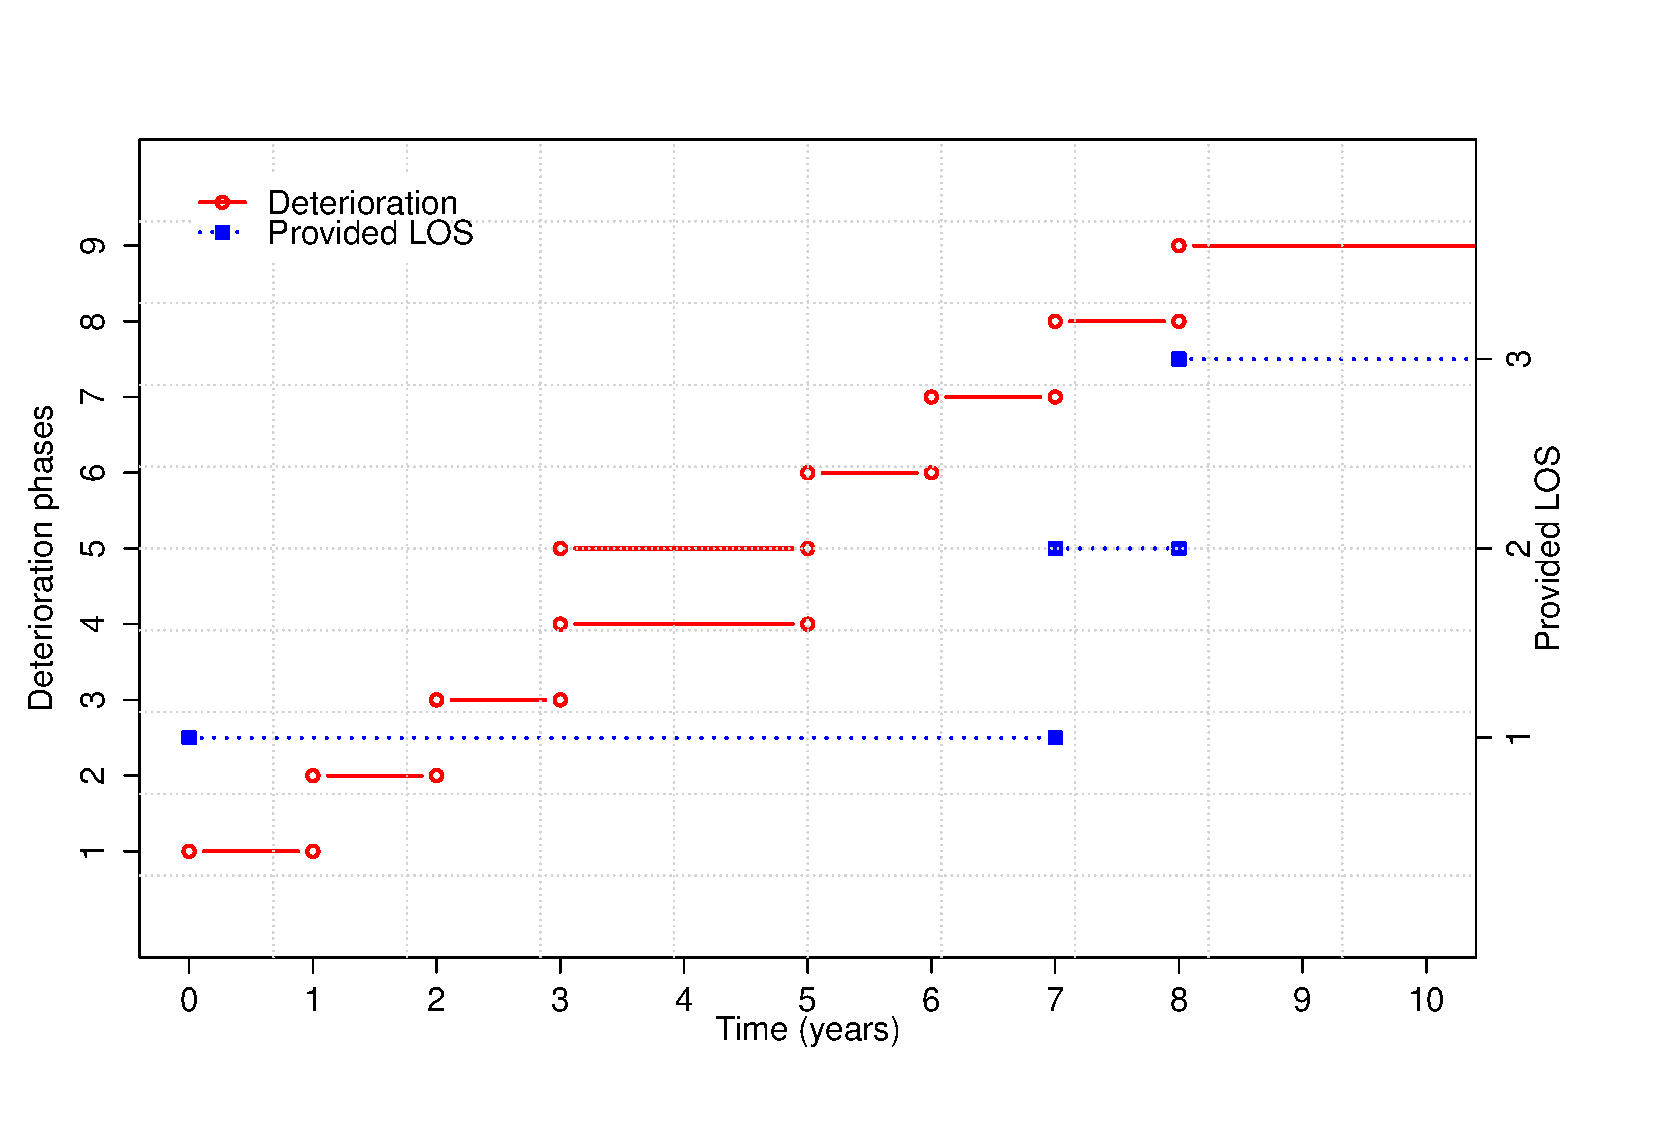
\includegraphics[width=376pt]{fig22.eps}
\caption{Illustration of relationship between deterioration processes and the provided LOS}\label{fig22}
\end{figure}

\subsection{Required LOSs}

Changes in required LOSs are the result of changing human needs. They often result in existing infrastructure providing an inadequate LOS. For example, if a bridge was designed to have two lanes but a decision was made to expand the road to four lanes to accommodate changing human needs, then the bridge would no longer provide an adequate LOS.

From an infrastructure managers perspective, processes that result in changes in required LOSs, as deterioration processes, can be classified as either manifest or latent. 

With respect to changes in required LOSs most processes are considered manifest if development strategies are well developed and triggers for the execution of interventions are determined. For example, the need to expand a road due to it reaching its carrying capacity in terms of number of vehicles in peak periods can be considered as a manifest process if the number of vehicles per hour are recorded every day and a development strategy has been determined that states that once the road is at 80\% its maximum capacity the road will be widened. 

Most processes are considered as latent if development strategies are not well developed and no triggers for the execution of interventions are determined. For example, if the infrastructure manager is focused simply on maintaining the physical condition of the road it may come to him as a surprise when suddenly politicians request that a certain road be widened. 

Some example of processes that can result in changes in the required LOS in buildings can be are shown in Table \ref{tbl:212}.

\begin{table}
\caption{Example changes for buildings and related processes}
\begin{tabular}{|l|l|ll}
\cline{1-2}
Change & Related process &  &  \\ 
\cline{1-2}
Floor space layout & Demand for apartments suitable for growing elderly population &  &  \\ 
\cline{1-2}
New windows & Demand for energy efficient houses and rises.  &  &  \\ 
\cline{1-2}
New heating system & Demand for less maintenance on the heating system &  &  \\ 
\cline{1-2}
New control system & Demand for better control over the quality of the indoor air condition. &  &  \\ 
\cline{1-2}
\end{tabular}
\label{tbl:212}
\end{table}

Changes to the required LOS can happen due the wishes of the owners of infrastructure or be imposed by external persons such as government. The government can also provide incentives for the owner to change the required LOS. Other stakeholders can exert influence on the owner to change the required LOS, e.g. tenants in an apartment building can threaten not to pay the rent unless an air conditioning system is installed. The development of new technologies can also instigate changes in the required LOS as new developments may make things possible that were not before, e.g. new heating systems.

\subsection{Methodology}

The five basic steps to modelling changes in the required LOS are (adapted from \cite{Neufville2011}):

\begin{itemize}
	\item \underline{Step 1}:  Identify key performance drivers, i.e. determine the things that if changed will result in a change in the required LOS, e.g. if the number of vehicles per day pass x, then the road will need to be widen.
	\item \underline{Step 2}: Analyse historical trends, i.e. obtain as much historical data as possible and model how it changed over time with the plan to use this model to predict the future values, e.g. obtain the evolution of vehicles on the road over the last 20 years.
	\item \underline{Step 3}: Identify trend breakers, i.e. dig deeper and try to determine if there is something that can be used to help you predict if this trend will continue or might change suddenly, e.g. a new rail link on which passenger trains will circulate is about to be completed where there was none before.
	\item \underline{Step 4}: Establish forecast accuracy, i.e. if enough data exists put yourself mentally in the past and see how could you have predicted the future for which you have data, e.g. using only traffic data from 1980 to 1999 how could would you be at predicting the traffic between 2000 and 2014. 
	\item \underline{Step 5}: Build a dynamic model, i.e. build a model that allows a range of predictions to be made using a sensible distribution. 
\end{itemize}

An example for a hospital is provided in  the work of \cite{Neufville2011} . 

More detail on model development will be provided later.

\section{Change in LOS-Example}

\subsection{Question C}

Using the owner and user impacts of the impact hierarchy developed in section 3, develop simple models to be used to estimate how the provided LOS of a road will change over 20 years to the relatively slow deterioration of the pavement surface. 

\subsection{Answer C}

\subsubsection{Background}

In order to develop simple models to quantify the values of the various impact types it is useful to think of the object under investigation as being in one of two states, i.e. when no intervention is being executed and when an intervention is being executed. In general, these can be represented by the functions $f_{}^k(t,x)$ and $g_{}^k(d,x)$, respectively (here, \textit{k} represents intervention to be executed, e.g. renewal of the road section; \textit{x} represents the performance indicator, \textit{t} and \textit{d} represent in between interventions and during intervention, respectively). It is assumed that they are expressed in \textit{mus}. Both can be given by functions that vary over time. For example, two following generic exponential functions which can be used are: 

\begin{eqnarray}
      && {f^k}(t,x) = {a^{k,x}} + {b^{k,x}} \cdot \exp ({\beta ^{k,x}} \cdot t) \label{fx}\\
      && {g^k}(d,x) = {\bar a^{k,x}} + {\bar b^{k,x}} \cdot \exp ({\bar \beta ^{k,x}} \cdot {d^k}) \label{gx}
\end{eqnarray}


Where  or ${f^k}(t,x)$ and $g_{}^k(d,x)$ represent the impacts (costs) that are incurred as a function of time (\textit{t} or \textit{d}) and parameters $a$, $b$, and $\beta $.

If it is assumed that the change in condition of the road over time is known, this equation links the changes any impact on any stakeholder to the change in condition of the road over time.  

An example of the evolution of vehicle operation cost (VoC) along with the evolution of roughness for 1 m length of road is shown in Figure \ref{fig23}. In the figure, Eq. (1) has parameter values \textit{a}=500, \textit{b}=800, and $\beta  = 0.095$. These values are often estimated using empirical models. For example, in order to estimate the evolution of the VoC in between two consecutive interventions (from ${t_1}$ to ${t_2}$), \cite{Ouyang2004} used the following function.

\begin{eqnarray}
      && \int\limits_{{t_1}}^{{t_2}} {{f^k}\left[ {s(t)} \right]} {e^{ - rt}}dt = c\int\limits_{{t_1}}^{{t_2}} {s(t){e^{ - rt}}} dt \label{stx}
\end{eqnarray}

In Eq. \eqref{stx}, $s(t)$ represents the roughness indicators; c is constant associated with cost; $r$ is discount factor. The functional form of the roughness can be estimated with a simple exponential function as follows:

\begin{eqnarray}
      && s(t) = s({t_0}) \cdot \exp \left[ {\alpha (t - {t_0})} \right] \hspace{2mm} (for \hspace{2mm} t \ge {t_0}) \label{stx1}
\end{eqnarray}


Where $s({t_0})$ is initial roughness indicator (the initial LOS) and $\alpha $is a deterioration parameter.

When the time \textit{t} is discrete, \cite{Ouyang2004} suggests to use following function

\begin{eqnarray}
      && s(t + 1) = \left[ {s(t) + \upsilon } \right] \cdot \exp (\alpha ) \label{stx2}
\end{eqnarray}

With $\upsilon $ is the pre-defined model's parameter.

The cost curve (green curve in Figure \ref{fig23}) represents the increase of vehicle operation cost over time. The discount rate used is 2\%. Evolution of roughness is estimated from using Eq. \eqref{stx2} with $\upsilon  = 2$ and $\alpha  = 0.0153$. Value of parameter $c$in Eq. \eqref{stx} is 2.1.

\begin{figure}[h]
\begin{center}
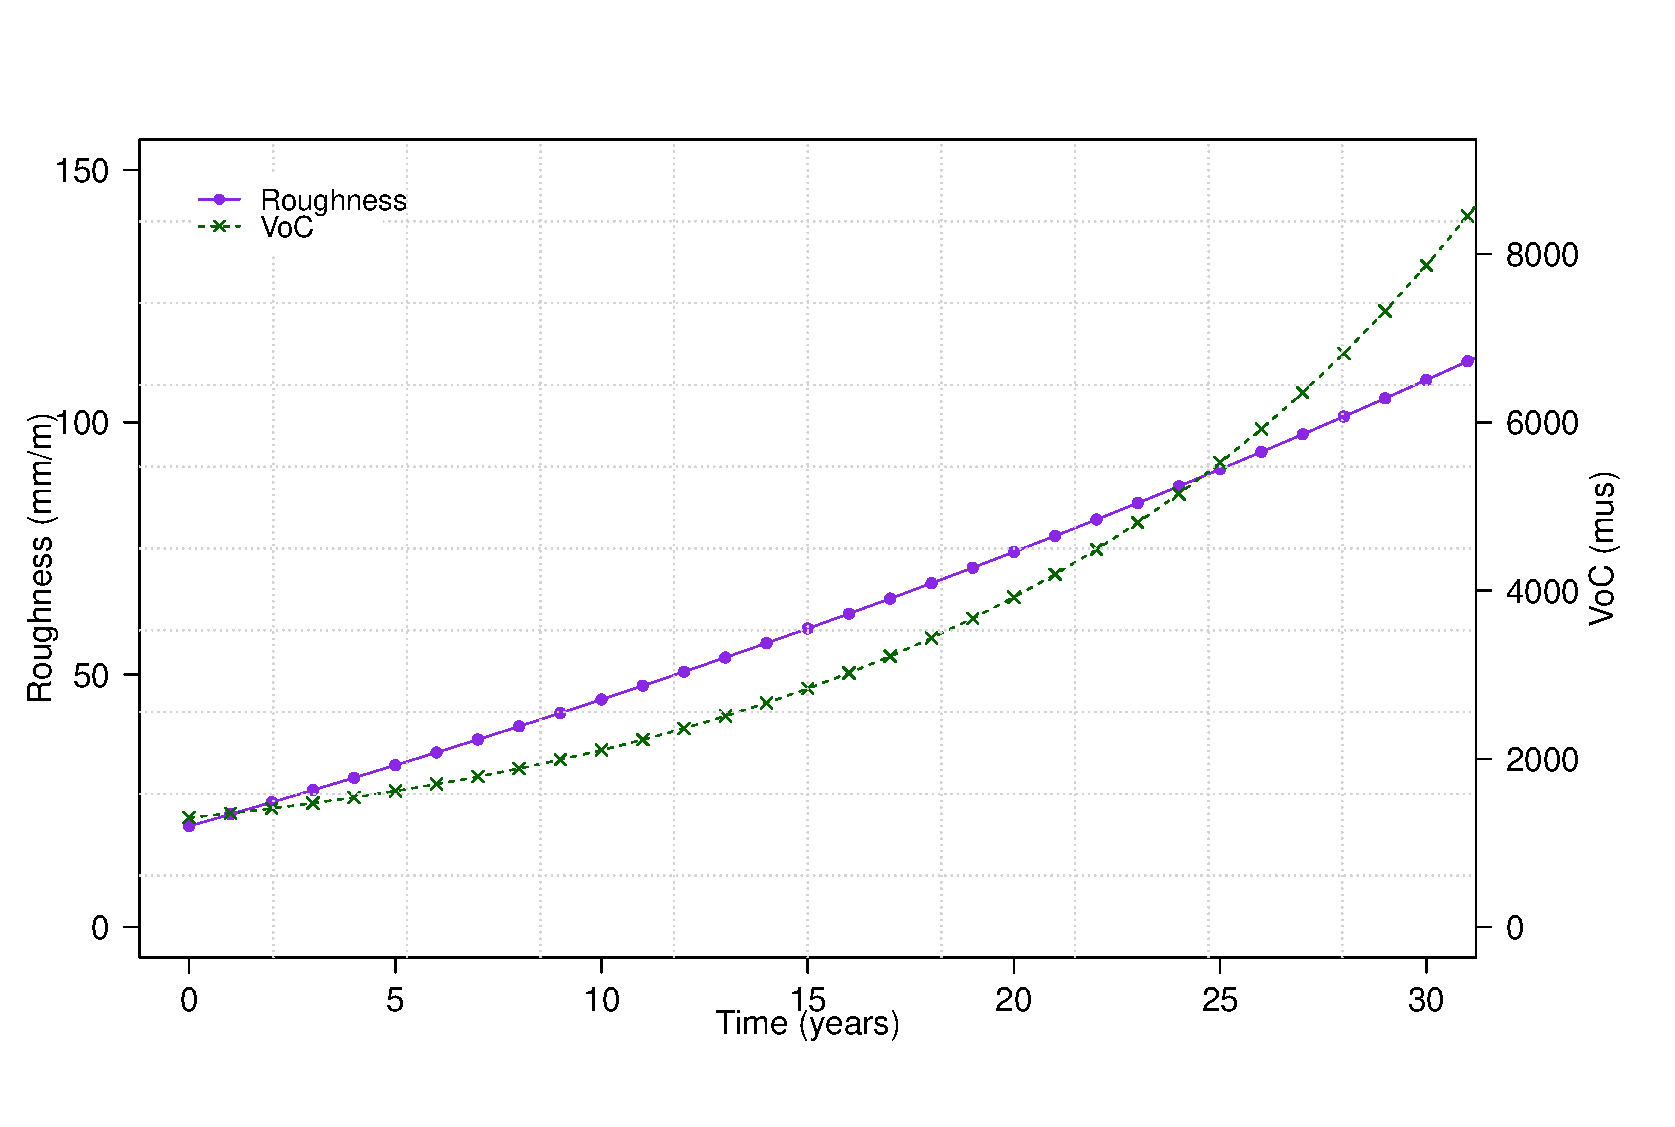
\includegraphics[width=402pt]{fig23.eps}
\caption{Evolution of VoC and roughness indicator}\label{fig23}
\end{center}
\end{figure}
 
Being generic, Eqs. \eqref{fx} and \eqref{gx} can be used to model the evolution of any impact that varies as a function of the condition of a road section, and allows the heterogeneity of each road section, e.g. the different deterioration rates, to be taken into consideration. For example, if it is desired to model the relationship between impacts on the user and the condition of a road section, the values of a, b, and \textit{$\beta{}$} (e.g. for user) could be selected as non-negative values, ensuring that the function \textit{f }will result in the values of the impact on the users that increase exponentially with time. This is similar to that of the user cost estimated using Eq. \eqref{stx}. Although the form of functions \textit{f} and \textit{g} are flexible, here, the exponential form is often used. 
%%%
\subsubsection{Owner}
%%%
\begin{eqnarray}
      && f_{}^k(t,x_i^o) = \sum\limits_{i = 1}^3 {I_i^o(t) \cdot c_i^o(t)} \label{fx1}\\
      && g_{}^k(d,x_i^o) = \sum\limits_{j = 1}^3 {I_i^o(d) \cdot c_i^o(d)} \label{gx1}
\end{eqnarray}
Where:\\
%\begin{flushright}
\begin{adjustwidth}{1cm}{}
\begin{description}
\item[$i$:] is the index of impact types: labor, equipment, and materials
\item[$I_i^o$:] is the owner impact indicator for impact type i. In this case it is the number of person-hours, numbers of equipment use hours, and quantity of materials used for intervention
\item[$c_i^o(t)$ and $c_i^o(d)$:] are owner unit costs, which vary as a function of time $t$ and $d$
\end{description}
%\end{flushright}
\end{adjustwidth}
\subsubsection{Users}
\begin{eqnarray}
      && f_{}^k(t,x_i^u) = \sum\limits_{i = 1}^3 {I_i^u(t) \cdot c_i^u(t)} \label{fx2}\\
      && g_{}^k(d,x_i^u) = \sum\limits_{i = 1}^3 {I_i^u(d) \cdot c_i^u(d)} \label{gx2}
\end{eqnarray}
Where:
%\begin{flushright}
\begin{adjustwidth}{1cm}{}
\begin{description}
\item[$i$:] is the index of impact types
\item[$I_i^u$:] is the user impact indicator for impact type $i$ 
\item[$c_i^u(t)$ and $c_i^u(d)$:] are user unit costs, which vary as a function of time $t$ and $d$.
\end{description}
%\end{flushright}
\end{adjustwidth}
%%%
\paragraph{\underline{Safety}}
The values of impact indicators ($I_i^u(t)$and $I_i^u(d)$) are generally estimated through regression analysis using empirical models. In empirical models, values of impact indicators associated with accidents can be estimated by using the ``accident rate'' multiplied by the cost of the accidents if they occur. Both depend on multiple factors such as the condition of the road, daily traffic volume, the physical condition of the driver of the vehicle and environmental factors such as, the occurrence of poor weather that can effect accident rate. For example, a popular way to estimate the value of impact indicators is by use of following equation \citep{Lindenmann2008}.

\begin{eqnarray}
      && I_{property}^u = t \cdot DTV \cdot s \cdot \theta  \cdot \omega  \cdot \upsilon \label{safety1}
\end{eqnarray}
Where:
%\begin{flushright}
\begin{adjustwidth}{1cm}{}
\begin{description}
\item[$t$:] is the number of days,
\item[$DTV$:] is the daily traffic volume,
\item[$s$:] is the length of the object,
\item[$\theta$:] is the coefficient depending on the deterioration level of the civil infrastructure,
\item[$\omega$:] is the correction factor for accident rate, and
\item[$\upsilon$:] is the approximate numbers of vehicles involved in an accident.
\end{description}
%\end{flushright}
\end{adjustwidth}
According to \cite{tarko2000}, three ways commonly used to estimate the accident rate are 
\begin{enumerate}
	\item crash rate method, which recommends a rate of crash for a specific type of road, in specific location, and with specified level of traffic volume; 
	\item crash equation method, which relies on a functional form of traffic volume and engineering factors; 
	\item crash reduction factor method, which is an extension method of crash equation method, where the crash reduction factor is given by: 
\end{enumerate}

\begin{eqnarray}
      && f(X) = k \cdot Y \cdot {Q^\gamma } \cdot {e^{\beta x}} \label{safety2}
\end{eqnarray}
Where:
\begin{adjustwidth}{1cm}{}
\begin{description}
\item[$f(X)$:] is the crash reduction function,
\item[$k$:] is a constant,
\item[$Y, Q$:] are the exposure variables representing the temporal span of data and indicate the section length and traffic volume, respectively, 
\item[$\beta$:] is the an unknown parameter associated with the variable X.
\item[$X$:] is the variable vector of engineering factors, including the performance condition of the road.
\end{description}
%\end{flushright}
\end{adjustwidth}
After obtaining the accident rate related to the execution of an intervention for each intervention type on an each object (i.e. between and during interventions), the value of impact indicators $I_i^u(t)$ and can be calculated. 

For example, after the execution of an intervention, an asphalt road section of 20 km is renewed to be in condition state 1. The daily traffic volume is 600 vehicles/day. The accident rates during and after intervention are estimated to be 0.03\% and 0.005\% out of the total traffic volume in a day. The duration of the intervention is 30 days. It is assumed that the average number of vehicles involved in an accident are two. 
%
The expected total numbers of vehicles involved in accidents in a year after intervention will be:

$I^u_{property}(t=365) \hspace{1mm}days \hspace{1mm} =365\times600\times0.005\%\times2 \approx 22 \hspace{1mm}$ vehicles 
%

The expected total numbers of vehicles involved in accidents during intervention will be:

$I^u_{property}(d=30) \hspace{1mm}days \hspace{1mm} =30\times600\times0.03\%\times2 \approx 11 \hspace{1mm}$ vehicles

The average unit cost $c_{{\rm{property}}}^u(t)$per vehicle can be approximated from historical data \cite{Lindberg1999}. 

\paragraph{\underline{Operation efficiency}}

The values of the travel time impact indicator can be approximated as a function of multiple factors including vehicle speed, amount of congestion, and curviness of the road. 

The values of the vehicle operation and maintenance impact indicators can be approximated as a function of multiple factors including the total number of vehicle type \textit{j}. (type $j$ means type of vehicles such as car, truck, bus, etc), 
\begin{eqnarray}
      && f^{k_{n_l}}_{n_l}(t,x^u_i)=I^u_{i,k_{n_l}} = \sum_{i=1}^2\sum_{j=1}^J C^u_{ij}(t) \cdot VH_j (t) \label{operation1}\\
      && g^{k_{n_l}}_{n_l}(d,x^u_i)=I^u_{i,k_{n_l}} = \sum_{i=1}^2\sum_{j=1}^J C^u_{ij}(d) \cdot VH_j (d) \label{operation2}
\end{eqnarray}
Where:
\begin{adjustwidth}{1cm}{}
\begin{description}
\item[$I_i^u$:] is the impact indicator for the index \textit{i}
\item[$i$:] is the index for vehicle maintenance cost and vehicle operation cost.
\item[$VH$:] is total number of vehicle type \textit{j}. (type \textit{\underline{j}} means type of vehicles such as car, truck, bus, etc). The value of \textit{VH} can be obtained from examining historical record on traffic volume and annual growth of traffic volume.
\end{description}
%\end{flushright}
\end{adjustwidth}
%
The value of $C_{ij}^u(t)$can be estimated by empirical study or regression analysis based on recorded numbers of bill paid for operation and maintenance respectively. To date, several models have been developed to relate such cost to deterioration or performance of the road. For example,\cite{OpusCL1999} studied the relationship between vehicle operation cost and international roughness index. The value of \textit{VH} can be obtained from examining historical record on traffic volume and annual growth of traffic volume.
%
\paragraph{\underline{Operational Quality}}
Impact indicators associated with and  can be measured by using qualitative scale (e.g, scale from 1 to 5, with 1 is the best and 5 is the worst) or by carrying out an empirical study on the loss in effective working time if users travel on a target road link. The values of the differences between these states in these scales can be determined through willing to pay investigations. 

Following proposed function can be used for estimating the values of impact indicators $BI^u_{physical, k_{n_l}}$ and $BI^u_{psychological, k_{n_l}}$.
\begin{eqnarray}
      && BI^u_{i,k_{n_l}} = t\cdot U\cdot \mu_i \label{operation3}
\end{eqnarray}
Where:
\begin{adjustwidth}{1cm}{}
\begin{description}
\item[$t$:] is the number of days,
\item[$U$:] is expected number of users per day, which can be approximated by means of daily traffic volume,
\item[$\mu$:] is the mean value of amount of physical and psychological impacts. It can be obtained by carrying out surveys on a population sample of the users.
\end{description}
%\end{flushright}
\end{adjustwidth}

For example, a survey using qualitative method on 300 users, who travel on a certain road link of 20 km, reveals a mean value $\mu_{physical}=3.4$ (from a scale of 5) per 1 km. The daily users have a factor of 2.5 times the daily traffic volume, which is 600 vehicles/day. Thus, in 30 days, the values of $I^u_{physical}=3.4$ will be determined as:

$I^u_{physical} = 30 \times (600 \times 2.5) \times 3.4 = 153'000 $ units

If each unit of physical impact is relatively cost 0.05 $mus$, then in total 30 days, the cost incurred to users due to physical impact will be $0.05(mus/unit)\times 153'000 (units)=7'650$  (mus).

\paragraph{Environment preservation (reduction of noise)}

Impact indicators associated with $I_{noise}^u$ can be approximated by use of following equation.

\begin{eqnarray}
      && I^u_{noise} = t\cdot \overline{dBA} \cdot U \label{operation4}
\end{eqnarray}
Where:
\begin{adjustwidth}{1cm}{}
\begin{description}
\item[$t$:] are the number of days in between interventions and during intervention,
\item[$\overline{dBA}$:] is the expected increase unit of noise (in $dBA$).
\item[$U$:] is the expected number of users within a specific period.
\end{description}
%\end{flushright}
\end{adjustwidth}

For example, an intervention is scheduled to last 30 days. The expected numbers of users could be estimated as 300 persons. If during intervention, the noise due to construction activities increases by 2 $dBA$ compared to the normal day without intervention, and one additional dBA has a value of 100 mus. Using Eq. \eqref{operation4}, the values of impact indicator will be

$I^u_{noise}=30 \times 2 \time 300 = 18'000 dBA-person-days$

and thus, the values of function $g^d(d,x^u_{noise})$ will be 

$g^d(d,x^u_{noise}) = 18'000 \times 100 = 1'800'000 \hspace {1mm} mus$
%
\section{Assignments}
\subsection{Problem A}
In class an impact hierarchy was given to be used to determine optimal intervention strategies and work programs for a road network. Discuss the suitability of this impacts hierarchy if it was to be used to determine optimal intervention strategies and work programs for 
\begin{adjustwidth}{1cm}{}
\begin{itemize}
\item[a)] a private road network, and 
\item[b)] a public rail network.                         
\end{itemize}
\end{adjustwidth}
%
\subsection{Answer A-a}
No specific answer is provided. Please submit your answer to obtain feedback. 
\subsection{Answer A-b}
No specific answer is provided. Please submit your answer to obtain feedback. 
%
\subsection{Problem B}
Water is one of the fundamental needs of millions of people living in a megacity. Water of sufficient quality and quantity must be provided around the clock. In order to fulfill this need, a city depends on its water distribution infrastructure, which includes pipes made of different materials and laid at different times. These pipes are affected by processes of different types and deteriorate at different rates. The consequences related to pipe failure vary significantly depending on the type of failure, e.g. a pipe break, or a leaking pipe, as does the reaction time required to fix the pipe. For example, if a pipe breaks, a corrective intervention must be executed immediately, and if it is noticed that there is progressive water loss over time then a preventive intervention can be planned before there is an inadequate level of service.  Part of the water distribution network in mega-city Q is shown in Figure \ref{fig24}. The pipe characteristics are given in Table \ref{tbl:213}. 

\begin{figure}[h]
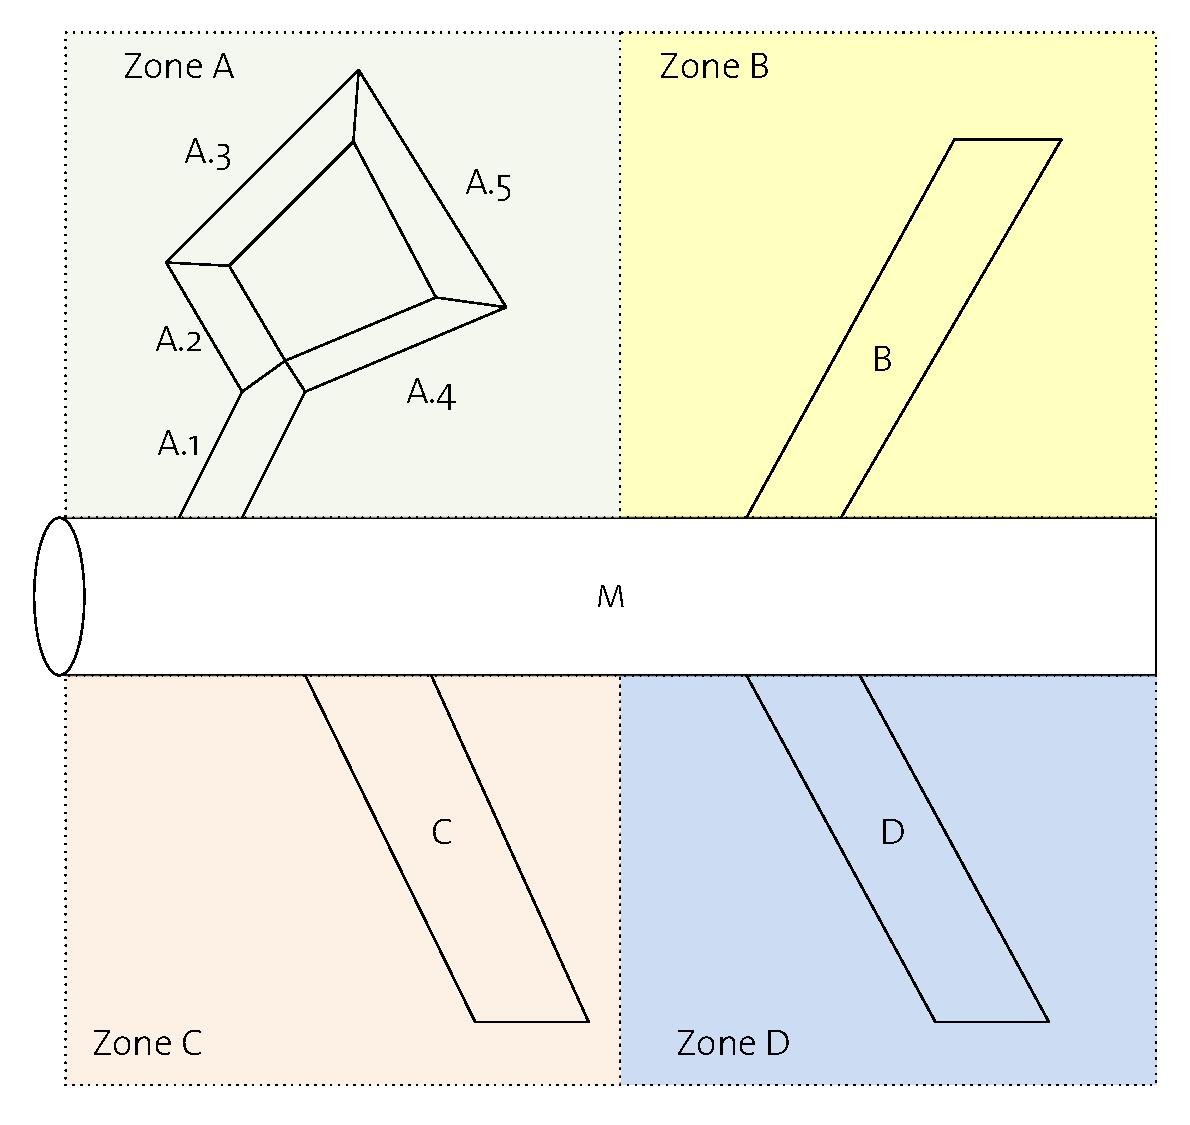
\includegraphics[width=200pt]{fig24.eps}
\caption{Simplified network of water supply pipes}\label{fig24}
\end{figure}


\begin{table}
\caption{Pipe and their attributes}
\begin{tabular}{|l|l|l|l|l|p{80pt}|}
\hline
\multicolumn{1}{|c|}{Pipe} & Material & \multicolumn{1}{c|}{Demand (m3/day)} & \multicolumn{1}{c|}{Length (m)} & \multicolumn{1}{c|}{Year of construction} & Usage \\ 
\hline
\multicolumn{1}{|c|}{M} & Concrete & \multicolumn{1}{c|}{} & \multicolumn{1}{c|}{5'000} & \multicolumn{1}{c|}{1998} & Distribution only \\ 
\hline
\multicolumn{1}{|c|}{A.1} & PVC & \multicolumn{1}{c|}{250'000} & \multicolumn{1}{c|}{600} & \multicolumn{1}{c|}{2003} & Distribution only \\ 
\cline{1-2}\cline{4-6}
\multicolumn{1}{|c|}{A.2} & PVC & \multicolumn{1}{c|}{} & \multicolumn{1}{c|}{600} & \multicolumn{1}{c|}{2003} & Distribution only \\ 
\cline{1-2}\cline{4-6}
\multicolumn{1}{|c|}{A.3} & PVC & \multicolumn{1}{c|}{} & \multicolumn{1}{c|}{600} & \multicolumn{1}{c|}{2003} & Distribution and connection to buildings \\ 
\cline{1-2}\cline{4-6}
\multicolumn{1}{|c|}{A.4} & PVC & \multicolumn{1}{c|}{} & \multicolumn{1}{c|}{600} & \multicolumn{1}{c|}{2003} & Distribution only \\ 
\cline{1-2}\cline{4-6}
\multicolumn{1}{|c|}{A.5} & PVC & \multicolumn{1}{c|}{} & \multicolumn{1}{c|}{600} & \multicolumn{1}{c|}{1998} & Distribution and connection to buildings \\ 
\hline
\multicolumn{1}{|c|}{B} & Cast iron type 1 & \multicolumn{1}{c|}{200'000} & \multicolumn{1}{c|}{2'500} & \multicolumn{1}{c|}{1993} & Distribution and connection to buildings \\ 
\hline
\multicolumn{1}{|c|}{C} & Cast iron type 2 & \multicolumn{1}{c|}{100'000} & \multicolumn{1}{c|}{1'600} & \multicolumn{1}{c|}{1993} & Distribution and connection to buildings \\ 
\hline
\multicolumn{1}{|c|}{D} & Cast iron type 3 & \multicolumn{1}{c|}{350'000} & \multicolumn{1}{c|}{4'000} & \multicolumn{1}{c|}{1983} & Distribution and connection to buildings \\ 
\hline
\end{tabular}
\label{tbl:213}
\end{table}
%
\subsection{Question B}
Make an impact hierarchy that you would use to measure the performance of the network. Be complete at the highest level, i.e. the stakeholders, and be detailed for one of the stakeholders besides the owner.
\subsection{Answer B}
No specific answer is provided. Please submit your answer to obtain feedback. 
\subsection{Problem C}
\subsection{Question C}
Using the impact hierarchy for public roads in the script explain three processes that would result in a change in a required level of service defined using accident costs, travel time costs and maintenance costs. 
\subsection{Answer C}
No specific answer is provided. Please submit your answer to obtain feedback. 
%
\bibliographystyle{plainnat}
\bibliography{reference}


\include{./Chapters/reliability}
%%%%%%%%%%%%%%%%%%%%% chapter.tex %%%%%%%%%%%%%%%%%%%%%%%%%%%%%%%%%
%
% sample chapter
%
% Use this file as a template for your own input.
%
%%%%%%%%%%%%%%%%%%%%%%%% Springer-Verlag %%%%%%%%%%%%%%%%%%%%%%%%%%
%\motto{Use the template \emph{chapter.tex} to style the various elements of your chapter content.}
\chapter{Availability and maintainability}
\label{avaimain} % Always give a unique label
% use \chaptermark{}
% to alter or adjust the chapter heading in the running head
\chapterauthor{Bryan T. Adey and Nam Lethanh}
\section{Maintainability of an item}
When managing infrastructure the maintainability of an item is often a useful
bit of information, i.e. how much effort is it to restore the item so that it
once again provides an adequate LOS. For example, if the speeds of trains need to
be reduced on a rail link due to deformations in a track, how much will it cost
to fix the rail link in a way that the trains can once again run at normal speed,
and how long will this take?

The maintainability of an item only has to do with the execution of
interventions on the item. The maintainability and reliability together give the
availability of an item.

\subsection{Time}
In order to estimate how long it will take to restore an item so that it
provides an adequate LOS, it is necessary to estimate the steps to be taken from
the instant that an inadequate LOS is not provided until it is restored. These
steps include the determination that a failure has occurred, the determination of
what exactly went wrong, the determination of how to restore the item, the
execution of the intervention, the testing that the item again can provide an
adequate LOS and then putting it back in operation so that it does provide an
adequate LOS. An illustration of this for the restoration of a part of an
electricity distribution network using Business Process Modelling Notation is
shown in Figure \ref{avaimain:1}.

\begin{figure}[h]
% \begin{center}
\includegraphics[width=450pt]{avaimain-1.eps}
\caption{Simplified process for the restoration of a part of an electricity
distribution network}\label{avaimain:1}
% \end{center}
\end{figure}
Once the process has been identified it is necessary to estimate the length of
time that each of the activities will take. This depends on many factors,
including the quantity and skill levels of persons required and available, the
quantity of required replacement parts required and available, and the amount of
time required to react to an indication that something is not working, sometimes
referred to as responsiveness.
\subsection{Indicators}
Indicators that are often used to express maintainability are the
mode\footnote{The duration or costs that occurs the most often},
mean\footnote{The average of the sum of all durations or costs divided by the
number of values} and maximum\footnote{The largest of all durations or costs
observed or expected. This is also often given as a percentile of the largest of
all durations or costs.} amount of duration or cost of interventions. Indicators
are usually developed for specific types of interventions, e.g. the mean duration
of a corrective intervention is 3 months, or the mean duration of a preventive
intervention is 1 week.
\section{Maintainability of an item comprised of sub-items}
The maintainability of an item can be estimated by taking into consideration the
structure of the sub-items in the item, and the maintainability of the sub-items.
This is advantageous if there is little data on the interventions that have been
executed on the item itself, e.g. a bridge, but abundant data on interventions
that have been executed on sub-items similar to those of which the item is
composed, e.g. a concrete abutment.

If it can be assumed that each intervention is only used to restore one sub-item
so that it provides an adequate LOS, the durations of the interventions can be
simply combined, e.g. if it takes 1 week to repair an abutment and 2 weeks to
repair a deck and both happen once every 10 years, the average time spent to
repair a bridge per year, i.e. its' maintainability, is 0.30 weeks ((1+2)/10).
If, however, 50\% of the time the abutment and deck are repaired at the same time
which takes 2 weeks, 50\% of the time they are repaired separately than the
average time spent to repair a bridge per year, i.e. its maintainability, is
0.175 weeks ((0.5(2)+0.25(1+2))/10).

The basic steps to combine sub-items, if it can be assumed that each
intervention is only used to restore one sub-item so that it provides an adequate
LOS, are:
\begin{itemize}
	\item divide all sub-items by type, so it can be assumed that each sub-item per
sub-item type behaves in the same way,
	\item determine the rate of occurrence of the type of intervention of interest, e.g.
corrective intervention, per sub-item type,
	\item estimate the rate of occurrence of the type of intervention, per sub-item type
by multiplying the rate of occurrence of the type of intervention by the number
of sub-items per sub-type,
	\item estimate the total duration of the type of intervention per sub-item type by
multiplying the rate of occurrence of the type of intervention by the mean
duration of the type of intervention per sub-item type
	\item estimate the rate of occurrence of an intervention on the item by summing the
rates of occurrence of the types of interventions per sub-item
	\item estimate the expected intervention duration, or maintainability, of the item by
summing the total duration of the type of intervention per sub-item.
\end{itemize}
\section{Availability of an item}
The availability of an item is based on both the reliability of an item and the
maintainability of an item. Simply, availability is:
\begin{eqnarray}
&& {A_i} = \frac{{E\left[ {t_i^{adequate}} \right]}}{{E\left[ {t_i^{adequate}}
\right] + E\left[ {t_i^{inadequate}} \right]}}
\label{avaimaineq:1}
%(1)
\end{eqnarray}
Where:
\begin{adjustwidth}{1cm}{}
\begin{description}
\item[$t_i^{adequate}$:] the duration of time item \textit{i} provides an adequate LOS,
\item[$t_i^{inadequate}$:] the duration of time item \textit{i} provides an inadequate LOS
\end{description}
%\end{flushright}
\end{adjustwidth}
When investigating the availability of an item the exact definition of
availability used is important. One should be explicit about
\begin{itemize}
	\item the types of interventions being considered, e.g. preventive and corrective
interventions or only corrective interventions
	\item the type of time being considered, e.g. is the time spent waiting for parts and
the time on-site to be considered, or only the time on-site.
\end{itemize}
Different measure of availability serve different purposes.
\subsection{Example}
A road has been in service for 10 years (3'652 days). Over those 10 years, 6
interventions have been executed. Some of those have been due to rock falls, some
due to scour and some due to chloride induced corrosion. The total amount of time
that an adequate LOS was not provided was 156 days, i.e. traffic flow was
restricted for 156 days in the last 3'652 days.
\subsubsection{Question A}
What was the availability of the road link?
\subsubsection{Answer A}
The total length of time when an adequate LOS was provided was 3'496 days (3'652
-- 156). The rate of occurrence of interventions was 0.001716 interventions/day
(6/3'496). The mean time between interventions is therefore 582.7 days
(1/0.001716). The availability is then
\begin{eqnarray}
&& \begin{array}{l}
 {A_i} = \frac{{E\left[ {t_i^a} \right]}}{{E\left[ {t_i^a} \right] + E\left[
{t_i^n} \right]}} = \frac{{582.7}}{{582.7 + 156/6}} = 0.9573
\end{array} \label{avaimaineq:2}
%(2)
\end{eqnarray}
\subsubsection{Question B}
Is this also the availability of the road next year?
\subsubsection{Answer B}
It depends on the types of failures and how they were repaired. In order to
state that the availability of the road next year is also 0.9573, it would be
necessary to be able to model the time between interventions as an exponential
distribution, meaning that rate of occurrence of failure can be modelled as
constant. This is essentially saying that no matter how many failure have
occurred in the past there will be on average the same number in the future. This
is in many cases not correct. For example, if there is an area in which a
landslide damages a road, it may be that there will never be another landslide in
this area. Or, if many interventions has to be executed due the corrosion of the
reinforcement in deck slabs and waterproofing layers on all than the number of
interventions per year in the future would change.
\section{Availability of an item comprised of sub-items}
In determining the availability of an item comprised of sub-items it is
important to explicitly take into consideration the structure of the item. The
availability of item \textit{i} comprised of sub-items connected in series is
given by:
\begin{eqnarray}
&& {A_i} = \prod\limits_j^J {\left( {\frac{{E\left[ {t_j^a} \right]}}{{E\left[
{t_j^a} \right] + E\left[ {t_j^n} \right]}}} \right)}
\label{avaimaineq:3}
%(3)
\end{eqnarray}
\subsection{Example}
You own a water distribution network that is connected as shown in Figure
\ref{avaimain:2}. The five pipes in the network have life expectancies of 20 years.
The life expectancies can be modelled using an exponential distribution. It takes
1 week to repair pipes 1 and 4, 2 weeks for pipes 2 and 5 and 3 weeks for pipe 3,
once it breaks.
\begin{figure}[h]
% \begin{center}
\includegraphics[width=450pt]{avaimain-2.eps}
\caption{Water distribution network}\label{avaimain:2}
% \end{center}
\end{figure}
\subsubsection{Question C}
What is the reliability of the network?
\subsubsection{Question D}
What is the availability of the network?
\subsubsection{Answer C}
Using the pivotal decomposition method, the structure function of the network is
\begin{eqnarray}
&& \begin{array}{l}
\phi (\vec x) = {x_1}{x_3}{x_4} + {x_1}{x_3}{x_5} + {x_2}{x_3}{x_4} +
{x_2}{x_3}{x_5} + {x_1}{x_2}{x_4}{x_5}\\
{\rm{          }} - {x_1}{x_2}{x_3}{x_4} - {x_1}{x_3}{x_4}{x_5} -
{x_1}{x_2}{x_3}{x_5} - {x_2}{x_3}{x_4}{x_5}
\end{array}
\label{avaimaineq:4}
%(4)
\end{eqnarray}
The steps to arrive at the above function has been described in section 3.3 of
the script of week 9.

In term of reliability, the structure function can be rewritten as
\begin{eqnarray}
&& \begin{array}{l}
{R_{network}}(t) = {R_1}(t) \cdot {R_3}(t) \cdot {R_4}(t) + {R_1}(t) \cdot
{R_3}(t) \cdot {R_5}(t) + {R_2}(t) \cdot {R_3}(t) \cdot {R_4}(t) + {R_2}(t) \cdot
{R_3}(t) \cdot {R_5}(t)\\
+ {R_1}(t) \cdot {R_2}(t) \cdot {R_4}(t) \cdot {R_5}(t){\rm{ }} - {R_1}(t)
\cdot {R_2}(t) \cdot {R_3}(t) \cdot {R_4}(t)\\
- {R_1}(t) \cdot {R_3}(t) \cdot {R_4}(t) \cdot {R_5}(t) - {R_1}(t) \cdot
{R_2}(t) \cdot {R_3}(t) \cdot {R_5}(t) - {R_2}(t) \cdot {R_3}(t) \cdot {R_4}(t)
\cdot {R_5}(t)
\end{array}
\label{avaimaineq:5}
%(5)
\end{eqnarray}
The reliability of any item \textit{i} at time \textit{t} is defined in \eqref{eqreliability:7}

As the expected time until an inadequate LOS is provided is about 20 years, the
``failure rate'' can be estimated as follows:

\[
 \int\limits_0^{ + \infty } {{R_i}(t)} dt = \int\limits_0^{ + \infty } {\exp
\left( { - {\theta _i} \cdot t} \right)dt}  = \frac{1}{{{\theta _i}}} = 20{\rm{
years}}
\]
\[
 {\theta _i} = \frac{1}{{20}} = 0.05
\]

Using equations \eqref{eqreliability:7} the reliability of each sub-item, and the item, in 30 years
can be estimated (Table \ref{tblavaimain:1}). For example, the probability that sub-item
1 will provide an adequate LOS until the start of year 14 is 0.522 and the
probability that the item will provide an adequate LOS until year 14 is 0.346.
This is illustrated in Figure \ref{avaimain:3}. Only one curve is used to represent
the reliability of a sub-item, since the reliability for all sub-items is the
same.
\begin{table}
\caption{Reliability}
\begin{tabular}{|l|l|l|l|l|l|l|}
\hline
\multicolumn{1}{|c|}{Time} & \multicolumn{6}{c|}{Reliability} \\ 
\cline{2-7}
\multicolumn{1}{|c|}{(years)} & \multicolumn{1}{c|}{1} & \multicolumn{1}{c|}{2} & \multicolumn{1}{c|}{3} & \multicolumn{1}{c|}{4} & \multicolumn{1}{c|}{5} & \multicolumn{1}{c|}{Item} \\ 
\hline
\multicolumn{1}{|c|}{1} & \multicolumn{1}{c|}{1} & \multicolumn{1}{c|}{1} & \multicolumn{1}{c|}{1} & \multicolumn{1}{c|}{1} & \multicolumn{1}{c|}{1} & \multicolumn{1}{c|}{1} \\ 
\hline
\multicolumn{1}{|c|}{2} & \multicolumn{1}{c|}{0.951} & \multicolumn{1}{c|}{0.951} & \multicolumn{1}{c|}{0.951} & \multicolumn{1}{c|}{0.951} & \multicolumn{1}{c|}{0.951} & \multicolumn{1}{c|}{0.987} \\ 
\hline
\multicolumn{1}{|c|}{3} & \multicolumn{1}{c|}{0.905} & \multicolumn{1}{c|}{0.905} & \multicolumn{1}{c|}{0.905} & \multicolumn{1}{c|}{0.905} & \multicolumn{1}{c|}{0.905} & \multicolumn{1}{c|}{0.952} \\ 
\hline
\multicolumn{1}{|c|}{4} & \multicolumn{1}{c|}{0.861} & \multicolumn{1}{c|}{0.861} & \multicolumn{1}{c|}{0.861} & \multicolumn{1}{c|}{0.861} & \multicolumn{1}{c|}{0.861} & \multicolumn{1}{c|}{0.904} \\ 
\hline
\multicolumn{1}{|c|}{5} & \multicolumn{1}{c|}{0.819} & \multicolumn{1}{c|}{0.819} & \multicolumn{1}{c|}{0.819} & \multicolumn{1}{c|}{0.819} & \multicolumn{1}{c|}{0.819} & \multicolumn{1}{c|}{0.847} \\ 
\hline
\multicolumn{1}{|c|}{6} & \multicolumn{1}{c|}{0.779} & \multicolumn{1}{c|}{0.779} & \multicolumn{1}{c|}{0.779} & \multicolumn{1}{c|}{0.779} & \multicolumn{1}{c|}{0.779} & \multicolumn{1}{c|}{0.786} \\ 
\hline
\multicolumn{1}{|c|}{7} & \multicolumn{1}{c|}{0.741} & \multicolumn{1}{c|}{0.741} & \multicolumn{1}{c|}{0.741} & \multicolumn{1}{c|}{0.741} & \multicolumn{1}{c|}{0.741} & \multicolumn{1}{c|}{0.723} \\ 
\hline
\multicolumn{1}{|c|}{8} & \multicolumn{1}{c|}{0.705} & \multicolumn{1}{c|}{0.705} & \multicolumn{1}{c|}{0.705} & \multicolumn{1}{c|}{0.705} & \multicolumn{1}{c|}{0.705} & \multicolumn{1}{c|}{0.66} \\ 
\hline
\multicolumn{1}{|c|}{9} & \multicolumn{1}{c|}{0.670} & \multicolumn{1}{c|}{0.670} & \multicolumn{1}{c|}{0.670} & \multicolumn{1}{c|}{0.670} & \multicolumn{1}{c|}{0.670} & \multicolumn{1}{c|}{0.599} \\ 
\hline
\multicolumn{1}{|c|}{10} & \multicolumn{1}{c|}{0.638} & \multicolumn{1}{c|}{0.638} & \multicolumn{1}{c|}{0.638} & \multicolumn{1}{c|}{0.638} & \multicolumn{1}{c|}{0.638} & \multicolumn{1}{c|}{0.541} \\ 
\hline
\multicolumn{1}{|c|}{11} & \multicolumn{1}{c|}{0.607} & \multicolumn{1}{c|}{0.607} & \multicolumn{1}{c|}{0.607} & \multicolumn{1}{c|}{0.607} & \multicolumn{1}{c|}{0.607} & \multicolumn{1}{c|}{0.487} \\ 
\hline
\multicolumn{1}{|c|}{12} & \multicolumn{1}{c|}{0.577} & \multicolumn{1}{c|}{0.577} & \multicolumn{1}{c|}{0.577} & \multicolumn{1}{c|}{0.577} & \multicolumn{1}{c|}{0.577} & \multicolumn{1}{c|}{0.436} \\ 
\hline
\multicolumn{1}{|c|}{13} & \multicolumn{1}{c|}{0.549} & \multicolumn{1}{c|}{0.549} & \multicolumn{1}{c|}{0.549} & \multicolumn{1}{c|}{0.549} & \multicolumn{1}{c|}{0.549} & \multicolumn{1}{c|}{0.389} \\ 
\hline
\multicolumn{1}{|c|}{14} & \multicolumn{1}{c|}{0.522} & \multicolumn{1}{c|}{0.522} & \multicolumn{1}{c|}{0.522} & \multicolumn{1}{c|}{0.522} & \multicolumn{1}{c|}{0.522} & \multicolumn{1}{c|}{0.346} \\ 
\hline
\multicolumn{1}{|c|}{15} & \multicolumn{1}{c|}{0.497} & \multicolumn{1}{c|}{0.497} & \multicolumn{1}{c|}{0.497} & \multicolumn{1}{c|}{0.497} & \multicolumn{1}{c|}{0.497} & \multicolumn{1}{c|}{0.307} \\ 
\hline
\multicolumn{1}{|c|}{16} & \multicolumn{1}{c|}{0.472} & \multicolumn{1}{c|}{0.472} & \multicolumn{1}{c|}{0.472} & \multicolumn{1}{c|}{0.472} & \multicolumn{1}{c|}{0.472} & \multicolumn{1}{c|}{0.272} \\ 
\hline
\multicolumn{1}{|c|}{17} & \multicolumn{1}{c|}{0.449} & \multicolumn{1}{c|}{0.449} & \multicolumn{1}{c|}{0.449} & \multicolumn{1}{c|}{0.449} & \multicolumn{1}{c|}{0.449} & \multicolumn{1}{c|}{0.241} \\ 
\hline
\multicolumn{1}{|c|}{18} & \multicolumn{1}{c|}{0.427} & \multicolumn{1}{c|}{0.427} & \multicolumn{1}{c|}{0.427} & \multicolumn{1}{c|}{0.427} & \multicolumn{1}{c|}{0.427} & \multicolumn{1}{c|}{0.212} \\ 
\hline
\multicolumn{1}{|c|}{19} & \multicolumn{1}{c|}{0.407} & \multicolumn{1}{c|}{0.407} & \multicolumn{1}{c|}{0.407} & \multicolumn{1}{c|}{0.407} & \multicolumn{1}{c|}{0.407} & \multicolumn{1}{c|}{0.187} \\ 
\hline
\multicolumn{1}{|c|}{20} & \multicolumn{1}{c|}{0.387} & \multicolumn{1}{c|}{0.387} & \multicolumn{1}{c|}{0.387} & \multicolumn{1}{c|}{0.387} & \multicolumn{1}{c|}{0.387} & \multicolumn{1}{c|}{0.164} \\ 
\hline
\multicolumn{1}{|c|}{21} & \multicolumn{1}{c|}{0.368} & \multicolumn{1}{c|}{0.368} & \multicolumn{1}{c|}{0.368} & \multicolumn{1}{c|}{0.368} & \multicolumn{1}{c|}{0.368} & \multicolumn{1}{c|}{0.144} \\ 
\hline
\multicolumn{1}{|c|}{22} & \multicolumn{1}{c|}{0.350} & \multicolumn{1}{c|}{0.350} & \multicolumn{1}{c|}{0.350} & \multicolumn{1}{c|}{0.350} & \multicolumn{1}{c|}{0.350} & \multicolumn{1}{c|}{0.126} \\ 
\hline
\multicolumn{1}{|c|}{23} & \multicolumn{1}{c|}{0.333} & \multicolumn{1}{c|}{0.333} & \multicolumn{1}{c|}{0.333} & \multicolumn{1}{c|}{0.333} & \multicolumn{1}{c|}{0.333} & \multicolumn{1}{c|}{0.111} \\ 
\hline
\multicolumn{1}{|c|}{24} & \multicolumn{1}{c|}{0.317} & \multicolumn{1}{c|}{0.317} & \multicolumn{1}{c|}{0.317} & \multicolumn{1}{c|}{0.317} & \multicolumn{1}{c|}{0.317} & \multicolumn{1}{c|}{0.097} \\ 
\hline
\multicolumn{1}{|c|}{25} & \multicolumn{1}{c|}{0.301} & \multicolumn{1}{c|}{0.301} & \multicolumn{1}{c|}{0.301} & \multicolumn{1}{c|}{0.301} & \multicolumn{1}{c|}{0.301} & \multicolumn{1}{c|}{0.085} \\ 
\hline
\multicolumn{1}{|c|}{26} & \multicolumn{1}{c|}{0.287} & \multicolumn{1}{c|}{0.287} & \multicolumn{1}{c|}{0.287} & \multicolumn{1}{c|}{0.287} & \multicolumn{1}{c|}{0.287} & \multicolumn{1}{c|}{0.074} \\ 
\hline
\multicolumn{1}{|c|}{27} & \multicolumn{1}{c|}{0.273} & \multicolumn{1}{c|}{0.273} & \multicolumn{1}{c|}{0.273} & \multicolumn{1}{c|}{0.273} & \multicolumn{1}{c|}{0.273} & \multicolumn{1}{c|}{0.064} \\ 
\hline
\multicolumn{1}{|c|}{28} & \multicolumn{1}{c|}{0.259} & \multicolumn{1}{c|}{0.259} & \multicolumn{1}{c|}{0.259} & \multicolumn{1}{c|}{0.259} & \multicolumn{1}{c|}{0.259} & \multicolumn{1}{c|}{0.056} \\ 
\hline
\multicolumn{1}{|c|}{29} & \multicolumn{1}{c|}{0.247} & \multicolumn{1}{c|}{0.247} & \multicolumn{1}{c|}{0.247} & \multicolumn{1}{c|}{0.247} & \multicolumn{1}{c|}{0.247} & \multicolumn{1}{c|}{0.049} \\ 
\hline
\multicolumn{1}{|c|}{30} & \multicolumn{1}{c|}{0.235} & \multicolumn{1}{c|}{0.235} & \multicolumn{1}{c|}{0.235} & \multicolumn{1}{c|}{0.235} & \multicolumn{1}{c|}{0.235} & \multicolumn{1}{c|}{0.043} \\ 
\hline
\end{tabular}
\label{tblavaimain:1}
\end{table}


\begin{figure}[h]
% \begin{center}
\includegraphics[width=415pt]{avaimain-3.eps}
\caption{Reliability and availability}\label{avaimain:3}
% \end{center}
\end{figure}
\subsubsection{Answer D}
The function form for calculating the availability is:
\begin{eqnarray}
&& \begin{array}{l}
{A_{network}}(t) = {A_1}(t) \cdot {A_3}(t) \cdot {A_4}(t) + {A_1}(t) \cdot
{A_3}(t) \cdot {A_5}(t) + {A_2}(t) \cdot {A_3}(t) \cdot {A_4}(t) + {A_2}(t) \cdot
{A_3}(t) \cdot {A_5}(t)\\
+ {A_1}(t) \cdot {A_2}(t) \cdot {A_4}(t) \cdot {A_5}(t){\rm{ }} - {A_1}(t)
\cdot {A_2}(t) \cdot {A_3}(t) \cdot {A_4}(t)\\
- {A_1}(t) \cdot {A_3}(t) \cdot {A_4}(t) \cdot {A_5}(t) - {A_1}(t) \cdot
{A_2}(t) \cdot {A_3}(t) \cdot {A_5}(t) - {A_2}(t) \cdot {A_3}(t) \cdot {A_4}(t)
\cdot {A_5}(t)
\end{array}
\label{avaimaineq:6}
%(9)
\end{eqnarray}
where ${A_i}(t)$is the availability of sub-item \textit{i}.

The availability of each sub-item is calculated with equation \eqref{avaimaineq:1}, in which, it
is necessary to calculate the mean time to repair or the mean time (duration) the
sub-item is in adequate level of service. This calculation involves the value of
reliability for each sub-item calculated in previous step.

\begin{eqnarray}
E(t_i^n) = {\Delta _i} \cdot {F_i}(t) = {\Delta _i} \cdot \left[ {1 - {R_i}(t)}
\right]
\label{avaimaineq:7}
%(10)
\end{eqnarray}


In equation \eqref{avaimaineq:7}, ${F_i}(t)$is the failure probability at time \textit{t}.

The availability of each sub-item in year \textit{t} will be
\begin{eqnarray}
A(t_i^{}) = \frac{{E\left[ {t_i^a} \right]}}{{E\left[ {t_i^a} \right] + E\left[
{t_i^n} \right]}} = \frac{{\int\limits_0^{tu} {{R_i}(t)dt} }}{{\int\limits_0^{tu}
{{R_i}(t)dt}  + {\Delta _i} \cdot \left[ {1 - {R_i}(tu)} \right]}}
\label{avaimaineq:8}
%(11)
\end{eqnarray}
The availability of each item and the network in 30 years.

Using equations \eqref{eqreliability:7} the availability of each sub-item, and the item, for periods
of time up to 30 years can be calculated (Table \ref{tblavaimain:2}). For example, the
availability of sub-item 1 for a 14 year time period is 0.999090421, and the
availability of the item for a 14 year time period is 0.999947505. This means
that on average over periods of time that are 14 years in length that one can
expect that sub-item 1 would provide an adequate LOS for 13.9872 years and an
inadequate LOS for 0.01273411 years (4.647949 days), and that the item would
provide an adequate LOS for 13.99927 years and an inadequate LOS for 0.00073
years (0.26645 days). The longer the period of time investigated the lower the
availability because the reliability of the sub-items decreases with age, when
there is a constant failure rate. This is illustrated in Figure \ref{avaimain:3}.

\begin{table}[h]
\caption{Availability}
\begin{tabular}{|l|l|l|l|l|l|l|}
\hline
\multicolumn{1}{|c|}{Time} & \multicolumn{6}{c|}{Availability} \\ 
\cline{2-7}
\multicolumn{1}{|c|}{(years)} & \multicolumn{1}{c|}{1} & \multicolumn{1}{c|}{2} & \multicolumn{1}{c|}{3} & \multicolumn{1}{c|}{4} & \multicolumn{1}{c|}{5} & \multicolumn{1}{c|}{Item} \\ 
\hline
\multicolumn{1}{|c|}{1} & \multicolumn{1}{c|}{1} & \multicolumn{1}{c|}{1} & \multicolumn{1}{c|}{1} & \multicolumn{1}{c|}{1} & \multicolumn{1}{c|}{1} & \multicolumn{1}{c|}{1} \\ 
\hline
\multicolumn{1}{|c|}{2} & \multicolumn{1}{c|}{0.999509} & \multicolumn{1}{c|}{0.999018} & \multicolumn{1}{c|}{0.997549} & \multicolumn{1}{c|}{0.998038} & \multicolumn{1}{c|}{0.998528} & \multicolumn{1}{c|}{0.999985} \\ 
\hline
\multicolumn{1}{|c|}{3} & \multicolumn{1}{c|}{0.999345} & \multicolumn{1}{c|}{0.998691} & \multicolumn{1}{c|}{0.996735} & \multicolumn{1}{c|}{0.997386} & \multicolumn{1}{c|}{0.998039} & \multicolumn{1}{c|}{0.999973} \\ 
\hline
\multicolumn{1}{|c|}{4} & \multicolumn{1}{c|}{0.999264} & \multicolumn{1}{c|}{0.998528} & \multicolumn{1}{c|}{0.996329} & \multicolumn{1}{c|}{0.997061} & \multicolumn{1}{c|}{0.997794} & \multicolumn{1}{c|}{0.999966} \\ 
\hline
\multicolumn{1}{|c|}{5} & \multicolumn{1}{c|}{0.999215} & \multicolumn{1}{c|}{0.998431} & \multicolumn{1}{c|}{0.996086} & \multicolumn{1}{c|}{0.996867} & \multicolumn{1}{c|}{0.997648} & \multicolumn{1}{c|}{0.999961} \\ 
\hline
\multicolumn{1}{|c|}{6} & \multicolumn{1}{c|}{0.999182} & \multicolumn{1}{c|}{0.998366} & \multicolumn{1}{c|}{0.995925} & \multicolumn{1}{c|}{0.996737} & \multicolumn{1}{c|}{0.997551} & \multicolumn{1}{c|}{0.999958} \\ 
\hline
\multicolumn{1}{|c|}{7} & \multicolumn{1}{c|}{0.999159} & \multicolumn{1}{c|}{0.99832} & \multicolumn{1}{c|}{0.995810} & \multicolumn{1}{c|}{0.996645} & \multicolumn{1}{c|}{0.997482} & \multicolumn{1}{c|}{0.999955} \\ 
\hline
\multicolumn{1}{|c|}{8} & \multicolumn{1}{c|}{0.999142} & \multicolumn{1}{c|}{0.998285} & \multicolumn{1}{c|}{0.995724} & \multicolumn{1}{c|}{0.996576} & \multicolumn{1}{c|}{0.99743} & \multicolumn{1}{c|}{0.999953} \\ 
\hline
\multicolumn{1}{|c|}{9} & \multicolumn{1}{c|}{0.999128} & \multicolumn{1}{c|}{0.998258} & \multicolumn{1}{c|}{0.995657} & \multicolumn{1}{c|}{0.996523} & \multicolumn{1}{c|}{0.99739} & \multicolumn{1}{c|}{0.999952} \\ 
\hline
\multicolumn{1}{|c|}{10} & \multicolumn{1}{c|}{0.999118} & \multicolumn{1}{c|}{0.998237} & \multicolumn{1}{c|}{0.995604} & \multicolumn{1}{c|}{0.99648} & \multicolumn{1}{c|}{0.997358} & \multicolumn{1}{c|}{0.999951} \\ 
\hline
\multicolumn{1}{|c|}{11} & \multicolumn{1}{c|}{0.999109} & \multicolumn{1}{c|}{0.998219} & \multicolumn{1}{c|}{0.995561} & \multicolumn{1}{c|}{0.996445} & \multicolumn{1}{c|}{0.997332} & \multicolumn{1}{c|}{0.99995} \\ 
\hline
\multicolumn{1}{|c|}{12} & \multicolumn{1}{c|}{0.999102} & \multicolumn{1}{c|}{0.998205} & \multicolumn{1}{c|}{0.995525} & \multicolumn{1}{c|}{0.996416} & \multicolumn{1}{c|}{0.99731} & \multicolumn{1}{c|}{0.999949} \\ 
\hline
\multicolumn{1}{|c|}{13} & \multicolumn{1}{c|}{0.999096} & \multicolumn{1}{c|}{0.998193} & \multicolumn{1}{c|}{0.995494} & \multicolumn{1}{c|}{0.996392} & \multicolumn{1}{c|}{0.997292} & \multicolumn{1}{c|}{0.999948} \\ 
\hline
\multicolumn{1}{|c|}{14} & \multicolumn{1}{c|}{0.99909} & \multicolumn{1}{c|}{0.998182} & \multicolumn{1}{c|}{0.995469} & \multicolumn{1}{c|}{0.996372} & \multicolumn{1}{c|}{0.997276} & \multicolumn{1}{c|}{0.999948} \\ 
\hline
\multicolumn{1}{|c|}{15} & \multicolumn{1}{c|}{0.999086} & \multicolumn{1}{c|}{0.998174} & \multicolumn{1}{c|}{0.995446} & \multicolumn{1}{c|}{0.996354} & \multicolumn{1}{c|}{0.997263} & \multicolumn{1}{c|}{0.999947} \\ 
\hline
\multicolumn{1}{|c|}{16} & \multicolumn{1}{c|}{0.999082} & \multicolumn{1}{c|}{0.998166} & \multicolumn{1}{c|}{0.995427} & \multicolumn{1}{c|}{0.996338} & \multicolumn{1}{c|}{0.997251} & \multicolumn{1}{c|}{0.999947} \\ 
\hline
\multicolumn{1}{|c|}{17} & \multicolumn{1}{c|}{0.999079} & \multicolumn{1}{c|}{0.998159} & \multicolumn{1}{c|}{0.995410} & \multicolumn{1}{c|}{0.996325} & \multicolumn{1}{c|}{0.997241} & \multicolumn{1}{c|}{0.999946} \\ 
\hline
\multicolumn{1}{|c|}{18} & \multicolumn{1}{c|}{0.999076} & \multicolumn{1}{c|}{0.998153} & \multicolumn{1}{c|}{0.995395} & \multicolumn{1}{c|}{0.996313} & \multicolumn{1}{c|}{0.997232} & \multicolumn{1}{c|}{0.999946} \\ 
\hline
\multicolumn{1}{|c|}{19} & \multicolumn{1}{c|}{0.999073} & \multicolumn{1}{c|}{0.998148} & \multicolumn{1}{c|}{0.995382} & \multicolumn{1}{c|}{0.996302} & \multicolumn{1}{c|}{0.997224} & \multicolumn{1}{c|}{0.999945} \\ 
\hline
\multicolumn{1}{|c|}{20} & \multicolumn{1}{c|}{0.999071} & \multicolumn{1}{c|}{0.998143} & \multicolumn{1}{c|}{0.99537} & \multicolumn{1}{c|}{0.996293} & \multicolumn{1}{c|}{0.997217} & \multicolumn{1}{c|}{0.999945} \\ 
\hline
\multicolumn{1}{|c|}{21} & \multicolumn{1}{c|}{0.999068} & \multicolumn{1}{c|}{0.998139} & \multicolumn{1}{c|}{0.995359} & \multicolumn{1}{c|}{0.996284} & \multicolumn{1}{c|}{0.99721} & \multicolumn{1}{c|}{0.999945} \\ 
\hline
\multicolumn{1}{|c|}{22} & \multicolumn{1}{c|}{0.999066} & \multicolumn{1}{c|}{0.998135} & \multicolumn{1}{c|}{0.99535} & \multicolumn{1}{c|}{0.996276} & \multicolumn{1}{c|}{0.997205} & \multicolumn{1}{c|}{0.999945} \\ 
\hline
\multicolumn{1}{|c|}{23} & \multicolumn{1}{c|}{0.999065} & \multicolumn{1}{c|}{0.998131} & \multicolumn{1}{c|}{0.995341} & \multicolumn{1}{c|}{0.996269} & \multicolumn{1}{c|}{0.997199} & \multicolumn{1}{c|}{0.999945} \\ 
\hline
\multicolumn{1}{|c|}{24} & \multicolumn{1}{c|}{0.999063} & \multicolumn{1}{c|}{0.998128} & \multicolumn{1}{c|}{0.995333} & \multicolumn{1}{c|}{0.996263} & \multicolumn{1}{c|}{0.997195} & \multicolumn{1}{c|}{0.999944} \\ 
\hline
\multicolumn{1}{|c|}{25} & \multicolumn{1}{c|}{0.999062} & \multicolumn{1}{c|}{0.998125} & \multicolumn{1}{c|}{0.995326} & \multicolumn{1}{c|}{0.996257} & \multicolumn{1}{c|}{0.99719} & \multicolumn{1}{c|}{0.999944} \\ 
\hline
\multicolumn{1}{|c|}{26} & \multicolumn{1}{c|}{0.99906} & \multicolumn{1}{c|}{0.998123} & \multicolumn{1}{c|}{0.99532} & \multicolumn{1}{c|}{0.996252} & \multicolumn{1}{c|}{0.997186} & \multicolumn{1}{c|}{0.999944} \\ 
\hline
\multicolumn{1}{|c|}{27} & \multicolumn{1}{c|}{0.999059} & \multicolumn{1}{c|}{0.99812} & \multicolumn{1}{c|}{0.995314} & \multicolumn{1}{c|}{0.996247} & \multicolumn{1}{c|}{0.997183} & \multicolumn{1}{c|}{0.999944} \\ 
\hline
\multicolumn{1}{|c|}{28} & \multicolumn{1}{c|}{0.999058} & \multicolumn{1}{c|}{0.998118} & \multicolumn{1}{c|}{0.995308} & \multicolumn{1}{c|}{0.996243} & \multicolumn{1}{c|}{0.99718} & \multicolumn{1}{c|}{0.999944} \\ 
\hline
\multicolumn{1}{|c|}{29} & \multicolumn{1}{c|}{0.999057} & \multicolumn{1}{c|}{0.998116} & \multicolumn{1}{c|}{0.995303} & \multicolumn{1}{c|}{0.996239} & \multicolumn{1}{c|}{0.997176} & \multicolumn{1}{c|}{0.999944} \\ 
\hline
\multicolumn{1}{|c|}{30} & \multicolumn{1}{c|}{0.999056} & \multicolumn{1}{c|}{0.998114} & \multicolumn{1}{c|}{0.995298} & \multicolumn{1}{c|}{0.996235} & \multicolumn{1}{c|}{0.997174} & \multicolumn{1}{c|}{0.999943} \\ 
\hline
\end{tabular}
\label{tblavaimain:2}
\end{table}

The code to compute this example is given in the Appendix \ref{appavai-mai1}
\section{Trade-offs}
Indicators of performance are just that, indicators. One can minimize the amount
of time required to execute interventions on an item, i.e. maximize
maintainability, by constructing an expensive but easy to repair item. This would
most likely increase the availability of the item but may have little effect on
the reliability of the item.

One can maximize the reliability of an item by constructing an expensive but
difficult to repair item. This would most likely decrease the maintainability of
the item but may have little effect on the availability of the item.

Once can maximize the availability of an item by constructing an expensive item
that is fairly reliable and fairly easy to repair.

In each of these cases, however, the most important question for the
infrastructure manager is whether the improvements in reliability, availability
or maintainability are worth the money spent. For example, if a road has very
little traffic it may not be worthwhile to spend a large amount of money to
shorten the durations of interventions, to increase the reliability of the bridge
in the road, or to improve the availability of the road.
\subsection{Example}
You are the manager of a tunnel that is considering the construction of tunnel
with five possible configurations. Each configuration is comprised of five
components, but three of the components can be one of two different types. The
configurations to be considered, as well as the mean time between failures for
each component in each configuration, the initial cost of each configuration, and
the mean intervention duration are given in Table \ref{tblavaimain:3}.
\begin{table}[h]
\caption{Tunnel components}
\begin{tabular}{|l|l|l|l|l|l|l|}
\hline
\multicolumn{2}{|c|}{Components} & \multicolumn{1}{c|}{Option 1} & \multicolumn{1}{c|}{Option 2} & \multicolumn{1}{c|}{Option 3} & \multicolumn{1}{c|}{Option 4} & \multicolumn{1}{c|}{Option 5} \\ 
\hline
\multicolumn{1}{|c|}{No.} & Description & \multicolumn{5}{c|}{mean time between failures (years)} \\ 
\hline
\multicolumn{1}{|c|}{1} & a power supply system & \multicolumn{1}{c|}{245} & \multicolumn{1}{c|}{9'612} & \multicolumn{1}{c|}{245} & \multicolumn{1}{c|}{9'612} & \multicolumn{1}{c|}{9'612} \\ 
\hline
\multicolumn{1}{|c|}{2} & a ventilation system & \multicolumn{1}{c|}{4'819} & \multicolumn{1}{c|}{4'819} & \multicolumn{1}{c|}{36'955} & \multicolumn{1}{c|}{4'819} & \multicolumn{1}{c|}{36'955} \\ 
\hline
\multicolumn{1}{|c|}{3} & a fire services system & \multicolumn{1}{c|}{1.1x106} & \multicolumn{1}{c|}{1.1x106} & \multicolumn{1}{c|}{1.1x106} & \multicolumn{1}{c|}{1.1x106} & \multicolumn{1}{c|}{1.1x106} \\ 
\hline
\multicolumn{1}{|c|}{4} & a drainage system & \multicolumn{1}{c|}{1} & \multicolumn{1}{c|}{1} & \multicolumn{1}{c|}{1} & \multicolumn{1}{c|}{2'194} & \multicolumn{1}{c|}{2'194} \\ 
\hline
\multicolumn{1}{|c|}{5} & a central monitoring and control system & \multicolumn{1}{c|}{2.4x105} & \multicolumn{1}{c|}{2.4x105} & \multicolumn{1}{c|}{2.4x105} & \multicolumn{1}{c|}{2.4x105} & \multicolumn{1}{c|}{2.4x105} \\ 
\hline
\multicolumn{1}{|l}{} & Initial cost (mus) & \multicolumn{1}{c|}{0} & \multicolumn{1}{c|}{2} & \multicolumn{1}{c|}{4} & \multicolumn{1}{c|}{6} & \multicolumn{1}{c|}{12} \\ 
\hline
\multicolumn{1}{|l}{} & Mean intervention duration (tu) & \multicolumn{1}{c|}{0.25} & \multicolumn{1}{c|}{0.28} & \multicolumn{1}{c|}{0.3} & \multicolumn{1}{c|}{1.5} & \multicolumn{1}{c|}{2} \\ 
\hline
\end{tabular}
\label{tblavaimain:3}
\end{table}
\subsubsection{Question}
Which configuration has the highest reliability? The highest maintainability?
The highest availability? And which configuration results in the lowest overall
net costs over a 20 \textit{tu} time period?
\subsubsection{Answer}
\paragraph{Reliability}
In the estimation of the reliability of the tunnel item one first has to
recognize that the 5 sub-items are conceptually connected in series, i.e. if one
sub-item fails the item fails. The next step is to calculate the failure rate of
each component, which if it is assumed that the failures of each component
follows can be modelled using an exponential distribution, is 1/the mean time
between failures. These are shown in Table \ref{tblavaimain:4}.
${\theta _1}$ ${\theta _2}$ ${\theta _3}$ ${\theta _4}$ ${\theta _5}$
The mean time between failures for the tunnel is then 1 over the sum of the
failure rates as shown in equation \eqref{avaimaineq:9}:
\begin{eqnarray}
&& \frac{1}{{\sum\limits_i^I {{\theta _i}} }}
\label{avaimaineq:9}
%(12)
\end{eqnarray}
Where i is the index of tunnel components.

And the reliability of the tunnel in one year is given by:
\begin{eqnarray}
&& R = \exp \left[ { - \left( {\sum\limits_i^I {{\theta _i}} } \right) \cdot 1}
\right]
\label{avaimaineq:10}
%(13)
\end{eqnarray}
These values for each of the options are shown in Table \ref{tblavaimain:4}. It can be
seen that option 5 is the most reliable, although not significantly more reliable
than option 4.
\begin{table}[h]
\caption{Failure rates of tunnel components, and mean time between failure and reliability of the tunnel}
\begin{tabular}{|l|l|l|l|l|l|l|l|l|}
\hline
\multicolumn{1}{|c|}{Option} & \multicolumn{1}{c|}{Item} & \multicolumn{5}{c|}{Components} & \multicolumn{1}{m{1.2cm}|}{MTBF of Tunnel} & \multicolumn{1}{c|}{Reliability} \\ 
\cline{3-7}
\multicolumn{1}{|c|}{} & \multicolumn{1}{c|}{} & \multicolumn{1}{m{1.2cm}|}{Power Supply System} & \multicolumn{1}{m{1.2cm}|}{Ventilation System} & \multicolumn{1}{m{1.2cm}|}{Fire Services System} & \multicolumn{1}{m{1.2cm}|}{Drainage System} & \multicolumn{1}{m{1.5cm}|}{Central monitoring and control system} & \multicolumn{1}{c|}{} & \multicolumn{1}{c|}{} \\ 
\hline
\multicolumn{1}{|c|}{1} & \multicolumn{1}{c|}{MTBF (years)} & \multicolumn{1}{c|}{245} & \multicolumn{1}{c|}{4'819} & \multicolumn{1}{c|}{1.10E+06} & \multicolumn{1}{c|}{1} & \multicolumn{1}{c|}{2.40E+05} & \multicolumn{1}{c|}{1} & \multicolumn{1}{c|}{0.3663} \\ 
\cline{2-7}
\multicolumn{1}{|c|}{} & \multicolumn{1}{c|}{$\theta_1$} & \multicolumn{1}{c|}{4.08E-03} & \multicolumn{1}{c|}{2.08E-04} & \multicolumn{1}{c|}{9.09E-07} & \multicolumn{1}{c|}{1.00E+00} & \multicolumn{1}{c|}{4.17E-06} & \multicolumn{1}{c|}{} & \multicolumn{1}{c|}{} \\ 
\hline
\multicolumn{1}{|c|}{2} & \multicolumn{1}{c|}{MTBF (years)} & \multicolumn{1}{c|}{9'612} & \multicolumn{1}{c|}{4'819} & \multicolumn{1}{c|}{1.10E+06} & \multicolumn{1}{c|}{1} & \multicolumn{1}{c|}{2.40E+05} & \multicolumn{1}{c|}{1} & \multicolumn{1}{c|}{0.3678} \\ 
\cline{2-7}
\multicolumn{1}{|c|}{} & \multicolumn{1}{c|}{$\theta_2$} & \multicolumn{1}{c|}{1.04E-04} & \multicolumn{1}{c|}{2.08E-04} & \multicolumn{1}{c|}{9.09E-07} & \multicolumn{1}{c|}{1.00E+00} & \multicolumn{1}{c|}{4.17E-06} & \multicolumn{1}{c|}{} & \multicolumn{1}{c|}{} \\ 
\hline
\multicolumn{1}{|c|}{3} & \multicolumn{1}{c|}{MTBF (years)} & \multicolumn{1}{c|}{245} & \multicolumn{1}{c|}{36'955} & \multicolumn{1}{c|}{1.10E+06} & \multicolumn{1}{c|}{1} & \multicolumn{1}{c|}{2.40E+05} & \multicolumn{1}{c|}{1} & \multicolumn{1}{c|}{0.3664} \\ 
\cline{2-7}
\multicolumn{1}{|c|}{} & \multicolumn{1}{c|}{$\theta_3$} & \multicolumn{1}{c|}{4.08E-03} & \multicolumn{1}{c|}{2.71E-05} & \multicolumn{1}{c|}{9.09E-07} & \multicolumn{1}{c|}{1.00E+00} & \multicolumn{1}{c|}{4.17E-06} & \multicolumn{1}{c|}{} & \multicolumn{1}{c|}{} \\ 
\hline
\multicolumn{1}{|c|}{4} & \multicolumn{1}{c|}{MTBF (years)} & \multicolumn{1}{c|}{9'612} & \multicolumn{1}{c|}{4'819} & \multicolumn{1}{c|}{1.10E+06} & \multicolumn{1}{c|}{2'194} & \multicolumn{1}{c|}{2.40E+05} & \multicolumn{1}{c|}{1'295} & \multicolumn{1}{c|}{0.9992} \\ 
\cline{2-7}
\multicolumn{1}{|c|}{} & \multicolumn{1}{c|}{$\theta_4$} & \multicolumn{1}{c|}{1.04E-04} & \multicolumn{1}{c|}{2.08E-04} & \multicolumn{1}{c|}{9.09E-07} & \multicolumn{1}{c|}{4.56E-04} & \multicolumn{1}{c|}{4.17E-06} & \multicolumn{1}{c|}{} & \multicolumn{1}{c|}{} \\ 
\hline
\multicolumn{1}{|c|}{5} & \multicolumn{1}{c|}{MTBF (years)} & \multicolumn{1}{c|}{9'612} & \multicolumn{1}{c|}{36'955} & \multicolumn{1}{c|}{1.10E+06} & \multicolumn{1}{c|}{2'194} & \multicolumn{1}{c|}{2.40E+05} & \multicolumn{1}{c|}{1'689} & \multicolumn{1}{c|}{0.9994} \\ 
\cline{2-7}
\multicolumn{1}{|c|}{} & \multicolumn{1}{c|}{$\theta_5$} & \multicolumn{1}{c|}{1.04E-004} & \multicolumn{1}{c|}{2.71E-005} & \multicolumn{1}{c|}{9.09E-007} & \multicolumn{1}{c|}{4.56E-004} & \multicolumn{1}{c|}{4.17E-006} & \multicolumn{1}{c|}{} & \multicolumn{1}{c|}{} \\ 
\hline
\end{tabular}
\label{tblavaimain:4}
\end{table}
\paragraph{Maintainability}
In order to calculate the maintainability we can look simply at the average
length of time it will take to restore each configuration when it fails. It is
here clear that the configuration 1, which has an average down time of 0.25
months if it fails is the most maintainable. This can be seen in Table
\ref{tblavaimain:5}.
\begin{table}[h]
\caption{Initial cost vs reliability, maintainability, availability and net benefit of the five
configurations}
\begin{tabular}{|l|l|l|l|l|}
\hline
\multicolumn{1}{|c|}{Configuration} & \multicolumn{1}{c|}{Initial Cost} & \multicolumn{1}{c|}{Reliability} & \multicolumn{1}{c|}{Maintainability} & \multicolumn{1}{c|}{Availability} \\ 
\multicolumn{1}{|c|}{} & \multicolumn{1}{c|}{(mus)} & \multicolumn{1}{c|}{} & \multicolumn{1}{c|}{(months)} & \multicolumn{1}{c|}{} \\ 
\hline
\multicolumn{1}{|c|}{1} & \multicolumn{1}{c|}{0} & \multicolumn{1}{c|}{0.3663} & \multicolumn{1}{c|}{\cellcolor{blue!25} 0.25} & \multicolumn{1}{c|}{0.979506} \\ 
\hline
\multicolumn{1}{|c|}{2} & \multicolumn{1}{c|}{2} & \multicolumn{1}{c|}{0.3678} & \multicolumn{1}{c|}{0.28} & \multicolumn{1}{c|}{0.97759} \\ 
\hline
\multicolumn{1}{|c|}{3} & \multicolumn{1}{c|}{4} & \multicolumn{1}{c|}{0.3664} & \multicolumn{1}{c|}{0.3} & \multicolumn{1}{c|}{0.975512} \\ 
\hline
\multicolumn{1}{|c|}{4} & \multicolumn{1}{c|}{6} & \multicolumn{1}{c|}{0.9992} & \multicolumn{1}{c|}{1.5} & \multicolumn{1}{c|}{\cellcolor{blue!25}0.999903} \\ 
\hline
\multicolumn{1}{|c|}{5} & \multicolumn{1}{c|}{12} & \multicolumn{1}{c|}{\cellcolor{blue!25} 0.9994} & \multicolumn{1}{c|}{2} & \multicolumn{1}{c|}{0.999901} \\ 
\hline
\end{tabular}
\label{tblavaimain:5}
\end{table}
\paragraph{Availability}
The availability of each configuration is given by taking the mean time between
failures, i.e. the mean time the item works, and dividing it by the average time
it takes to restore the configuration if it fails plus the mean time it works,
i.e. the average amount of time from starting to providing an adequate LOS to
providing an adequate LOS again. One can also refer to this as the renewal
period. The configuration with the highest availability is configuration 4 (Table
\ref{tblavaimain:5}).

\paragraph{Costs}
The net costs are the initial costs plus the costs incurred over the 20 year
period due to the costs due to lost service when an inadequate LOS is provided,
which in this case are considered to include the cost of interventions when
executed. Assuming that these costs are directly and uniformly related to the
amount of time required to restore service, the annual maintenance costs for each
configuration are given by:
\begin{eqnarray}
&& {C_{am}} = \frac{{E\left[ {t_i^n} \right] \cdot {I_{cr}}/12}}{{E\left[ {t_i^a}
\right] + E\left[ {t_i^n} \right]}}
%(13)
\end{eqnarray}
Where \textit{I$_{cr}$} represents the cost of executing an intervention
multiplied by the probability of executing an intervention

The annual maintenance costs as well as the net benefit excluding upfront costs
and including upfront costs are shown for each configuration in Table
\ref{tblavaimain:6}. The net benefit of a configuration is the cost of configuration 1
minus the costs of the configuration being investigated. It can be seen that
configuration has the highest net benefit over the 20 \textit{tu} period.

\begin{eqnarray}
&& N{B^i} = NB_c^i + NB_m^i\,\,\,\,\,\,\,\,\,\, = \left( {C_c^r - C_c^i} \right) +
\left( {C_m^r - C_m^i} \right)
\label{avaimaineq:11}
%(15)
\end{eqnarray}
\begin{adjustwidth}{1cm}{}
\begin{description}
\item[$N{B^i}$:] is the net benefit of configuration i,
\item[$C_m^r$:] is the maintenance costs of the reference configuration
\item[$C_m^i$:] is the maintenance costs of configuration i
\end{description}
%\end{flushright}
\end{adjustwidth}

\begin{table}[h]
\caption{ Initial cost versus total costs of the five configurations}
\begin{tabular}{|l|l|l|l|l|l|l|l|}
\hline
\multicolumn{1}{|c|}{Configuration} & \multicolumn{5}{c|}{Cost} & \multicolumn{1}{c|}{Net benefit} & \multicolumn{1}{c|}{Net benefit} \\ 
\cline{2-6}
\multicolumn{1}{|c|}{} & \multicolumn{1}{c|}{initial} & \multicolumn{1}{c|}{ Cost} & \multicolumn{1}{c|}{Cost} & \multicolumn{1}{c|}{Cost per tu} & \multicolumn{1}{c|}{Cost for 20 tus} & \multicolumn{1}{c|}{excluding} & \multicolumn{1}{c|}{including} \\ 
\multicolumn{1}{|c|}{} & \multicolumn{1}{c|}{(mus)} & \multicolumn{1}{c|}{mus/month} & \multicolumn{1}{c|}{(mus)} & \multicolumn{1}{c|}{} & \multicolumn{1}{c|}{} & \multicolumn{1}{c|}{upfront costs} & \multicolumn{1}{c|}{upfront costs} \\ 
\multicolumn{1}{|c|}{} & \multicolumn{1}{c|}{$C_c$} & \multicolumn{1}{c|}{$I_{cr}$} & \multicolumn{1}{c|}{$E[t_i^n]\cdot I_{cr}$} & \multicolumn{1}{c|}{$C_{am}$} & \multicolumn{1}{c|}{$C_{am}\cdot 20$} & \multicolumn{1}{c|}{$NB_m^i$} & \multicolumn{1}{c|}{$NB^i$} \\ 
\hline
\multicolumn{1}{|c|}{1} & \multicolumn{1}{c|}{0} & \multicolumn{1}{c|}{5} & \multicolumn{1}{c|}{1.25} & \multicolumn{1}{c|}{$7.79x10^{-1}$} & \multicolumn{1}{c|}{15.5844} & \multicolumn{1}{c|}{0} & \multicolumn{1}{c|}{0} \\ 
\hline
\multicolumn{1}{|c|}{2} & \multicolumn{1}{c|}{2} & \multicolumn{1}{c|}{5} & \multicolumn{1}{c|}{1.38} & \multicolumn{1}{c|}{$8.50x10^{-1}$} & \multicolumn{1}{c|}{17.0023} & \multicolumn{1}{c|}{-1.418} & \multicolumn{1}{c|}{-3.418} \\ 
\hline
\multicolumn{1}{|c|}{3} & \multicolumn{1}{c|}{4} & \multicolumn{1}{c|}{5} & \multicolumn{1}{c|}{1.5} & \multicolumn{1}{c|}{$9.31x10^{-1}$} & \multicolumn{1}{c|}{18.6197} & \multicolumn{1}{c|}{-3.035} & \multicolumn{1}{c|}{-7.035} \\ 
\hline
\multicolumn{1}{|c|}{4} & \multicolumn{1}{c|}{6} & \multicolumn{1}{c|}{5} & \multicolumn{1}{c|}{7.5} & \multicolumn{1}{c|}{$4.47x10^{-6}$} & \multicolumn{1}{c|}{0.0001} & \multicolumn{1}{c|}{15.584} & \multicolumn{1}{c|}{9.584} \\ 
\hline
\multicolumn{1}{|c|}{5} & \multicolumn{1}{c|}{12} & \multicolumn{1}{c|}{5} & \multicolumn{1}{c|}{10} & \multicolumn{1}{c|}{$3.50x10^{-6}$} & \multicolumn{1}{c|}{0.0001} & \multicolumn{1}{c|}{15.584} & \multicolumn{1}{c|}{3.584} \\ 
\hline
\end{tabular}
\label{tblavaimain:6}
\end{table}

\paragraph{Summary}
As can be seen in Table \ref{tblavaimain:7} that estimating the availability was the
only performance indicator that allowed the optimal configuration to be
determined. This will, however, not always be the case. This should be kept in
mind when selecting performance indicators to evaluate performance.
\begin{table}[h]
\caption{Initial cost vs reliability, maintainability, availability and net benefit of the five
configurations}
\begin{tabular}{|l|l|l|l|l|l|}
\hline
\multicolumn{1}{|c|}{Configuration} & \multicolumn{1}{c|}{Initial Cost} & \multicolumn{1}{c|}{Reliability} & \multicolumn{1}{c|}{Maintainability} & \multicolumn{1}{c|}{Availability} & \multicolumn{1}{c|}{Net benefit} \\ 
\multicolumn{1}{|c|}{} & \multicolumn{1}{c|}{(mus)} & \multicolumn{1}{c|}{} & \multicolumn{1}{c|}{(months)} & \multicolumn{1}{c|}{} & \multicolumn{1}{c|}{including upfront costs} \\ 
\hline
\multicolumn{1}{|c|}{1} & \multicolumn{1}{c|}{0} & \multicolumn{1}{c|}{0.3663} & \multicolumn{1}{c|}{\cellcolor{blue!25} 0.25} & \multicolumn{1}{c|}{0.979506} & \multicolumn{1}{c|}{0.000} \\ 
\hline
\multicolumn{1}{|c|}{2} & \multicolumn{1}{c|}{2} & \multicolumn{1}{c|}{0.3678} & \multicolumn{1}{c|}{0.28} & \multicolumn{1}{c|}{0.97759} & \multicolumn{1}{c|}{-3.418} \\ 
\hline
\multicolumn{1}{|c|}{3} & \multicolumn{1}{c|}{4} & \multicolumn{1}{c|}{0.3664} & \multicolumn{1}{c|}{0.3} & \multicolumn{1}{c|}{0.975512} & \multicolumn{1}{c|}{-7.035} \\ 
\hline
\multicolumn{1}{|c|}{4} & \multicolumn{1}{c|}{6} & \multicolumn{1}{c|}{0.9992} & \multicolumn{1}{c|}{1.5} & \multicolumn{1}{c|}{\cellcolor{blue!25} 0.999903} & \multicolumn{1}{c|}{\cellcolor{blue!25} 9.584} \\ 
\hline
\multicolumn{1}{|c|}{5} & \multicolumn{1}{c|}{12} & \multicolumn{1}{c|}{\cellcolor{blue!25} 0.9994} & \multicolumn{1}{c|}{2} & \multicolumn{1}{c|}{0.999901} & \multicolumn{1}{c|}{3.584} \\ 
\hline
\end{tabular}
\label{tblavaimain:7}
\end{table}
The R code for this example is given in Appendix \ref{appavai-mai2}

\section{Assignments}
\subsection{Problem A}
An infrastructure manager is responsible for maintaining a number of
facilities over a period of time. The length of time required for past corrective
interventions are given in Table \ref{tblavaimain:8}

\begin{table}[h]
\caption{ Corrective maintenance task times}
\begin{tabular}{|c|c|}
\hline
Task time & Frequency \\ 
\hline
11 & 2 \\ 
\hline
13 & 3 \\ 
\hline
15 & 8 \\ 
\hline
17 & 12 \\ 
\hline
19 & 12 \\ 
\hline
21 & 14 \\ 
\hline
23 & 13 \\ 
\hline
25 & 10 \\ 
\hline
27 & 10 \\ 
\hline
29 & 8 \\ 
\hline
31 & 7 \\ 
\hline
33 & 6 \\ 
\hline
35 & 5 \\ 
\hline
36 & 5 \\ 
\hline
37 & 4 \\ 
\hline
39 & 3 \\ 
\hline
41 & 2 \\ 
\hline
47 & 2 \\ 
\hline
\end{tabular}
\label{tblavaimain:8}
\end{table}
\subsubsection{Question A1}
What is the range of observations?
\subsubsection{Answer A1}
The range of observations is the difference between the smallest and the
largest value in the data set. In this respect, the range of the above data set
is
\begin{eqnarray}
&& Range = \max (data) - \min (data)
\label{eqavaimain:1}
%(1)
\end{eqnarray}
\[
Range = 14 - 2 = 12
\]
\subsubsection{Question A2s}
Using a class interval of 4, determine the number of class intervals.
Plot the data and construct a curve. What is the most likely type of distribution
is indicated by the curve?
\subsubsection{Answer A2}
With a class interval of 4, one can construct a range of observations.
This is equivalent to the class interval of 4.

\begin{table}[h]
\caption{Range of observation}
\begin{tabular}{|l|l|}
\hline
\multicolumn{1}{|c|}{Range} & \multicolumn{1}{c|}{Frequency} \\ 
\hline
\multicolumn{1}{|c|}{9-12} & \multicolumn{1}{c|}{2} \\ 
\hline
\multicolumn{1}{|c|}{13-16} & \multicolumn{1}{c|}{11} \\ 
\hline
\multicolumn{1}{|c|}{17-20} & \multicolumn{1}{c|}{24} \\ 
\hline
\multicolumn{1}{|c|}{21-24} & \multicolumn{1}{c|}{27} \\ 
\hline
\multicolumn{1}{|c|}{25-28} & \multicolumn{1}{c|}{20} \\ 
\hline
\multicolumn{1}{|c|}{29-32} & \multicolumn{1}{c|}{15} \\ 
\hline
\multicolumn{1}{|c|}{33-36} & \multicolumn{1}{c|}{16} \\ 
\hline
\multicolumn{1}{|c|}{37-40} & \multicolumn{1}{c|}{7} \\ 
\hline
\multicolumn{1}{|c|}{41-44} & \multicolumn{1}{c|}{2} \\ 
\hline
\multicolumn{1}{|c|}{45-48} & \multicolumn{1}{c|}{2} \\ 
\hline
\end{tabular}
\label{tblavaimain:9}
\end{table}

From this table, a histogram of frequency can be constructed (Figure
\ref{figavaimain-a:1})

\begin{figure}[h]
% \begin{center}
\includegraphics[width=376pt]{avaimain-a-9.eps}
\caption{Histogram of data}\label{figavaimain-a:1}
% \end{center}
\end{figure}

By observing the shape of the histogram, one can conclude that the data
is distributed close to the density of the lognormal distribution function, which
has a skew tail on the right side of the density function.

The lognormal distribution function has following properties

Probability density function
\begin{eqnarray}
&& {f_X}(x,\mu ,\sigma ) = \frac{1}{{x \cdot \sigma \sqrt {2\pi } }}{e^{ -
\frac{{{{(\ln x - \mu )}^2}}}{{2{\sigma ^2}}}}}{\rm{,   }}x > 0
\label{eqavaimain:2}
%(2)
\end{eqnarray}
Cumulative distribution function
\begin{eqnarray}
&& {F_X}(x,\mu ,\sigma ) = \frac{1}{2} + \frac{1}{2}erf\left[ {\frac{{(\ln x - \mu
)}}{{\sqrt {2\sigma } }}} \right]
\label{eqavaimain:3}
%(3)
\end{eqnarray}
where:
\begin{adjustwidth}{1cm}{}
\begin{description}
\item[$x$:] is the random variable of the distribution,
\item[$\mu$:] is the mean of the variable's natural logarithm,
\item[$\sigma $:] is the standard deviation of the variable's natural logarithm,
\item[$erf $:] is the error function.
\end{description}
%\end{flushright}
\end{adjustwidth}
\subsubsection{Question A3}
What is the mean length of time for a corrective intervention,
\textit{M$_{ct}$}?
\subsubsection{Answer A3}
For estimating the mean corrective intervention duration
\begin{eqnarray}
&& {\overline M _{ct}} = \frac{{\sum {\left( {{f_{c{t_i}}}} \right)\left(
{{M_{c{t_i}}}} \right)} }}{{\sum {{f_{c{t_i}}}} }}
\label{eqavaimain:4}
%(4)
\end{eqnarray}
where:
\begin{adjustwidth}{1cm}{}
\begin{description}
\item[$f_{cti}$:] is the frequency of the \textit{i$^{th}$} corrective intervention in interventions per system operating time unit,
\item[$M_{cti}$:] is the elapsed time required for the \textit{i$^{th}$} corrective intervention.
\end{description}
%\end{flushright}
\end{adjustwidth}
The answer is 25.15 days
\begin{table}[h]
\caption{Mean time of intervention duration}
\begin{tabular}{|c|c|c|c|}
\hline
Time & Frequency & Mean time & Variance \\ 
\hline
(1) & (2) & (3)=(1)*(2) & $(4)=(2)*[(1)- \bar M_{ct}]^²$ \\ 
\hline
11 & 2 & 22 & 400.49 \\ 
\hline
13 & 3 & 39 & 442.93 \\ 
\hline
15 & 8 & 120 & 824.31 \\ 
\hline
17 & 12 & 204 & 797.23 \\ 
\hline
19 & 12 & 228 & 453.99 \\ 
\hline
21 & 14 & 294 & 241.21 \\ 
\hline
23 & 13 & 299 & 60.14 \\ 
\hline
25 & 10 & 250 & 0.23 \\ 
\hline
27 & 10 & 270 & 34.2 \\ 
\hline
29 & 8 & 232 & 118.53 \\ 
\hline
31 & 7 & 217 & 239.49 \\ 
\hline
33 & 6 & 198 & 369.66 \\ 
\hline
35 & 5 & 175 & 485.03 \\ 
\hline
36 & 5 & 180 & 588.53 \\ 
\hline
37 & 4 & 148 & 561.61 \\ 
\hline
39 & 3 & 117 & 575.4 \\ 
\hline
41 & 2 & 82 & 502.39 \\ 
\hline
47 & 2 & 94 & 954.78 \\ 
\hline
\textbf{Total} & \textbf{126} & \textbf{3'169} & \textbf{7'650.13} \\ 
\hline
\end{tabular}
\label{tblavaimain:10}
\end{table}
  \[
   {\overline M _{ct}} = \frac{{3'169}}{{126}} = 25.15
  \]
\subsubsection{Question A4}
What is the geometric mean of the repair times?
\subsubsection{Answer A4}
For calculating geometric mean, refer to general statistical materials
\begin{eqnarray}
&& {\bar \mu _{geo}} = {e^\mu }
\label{eqavaimai:5}
%(4)
\end{eqnarray}
Where $\mu{}$ is the mean that is calculated based on the mean ${\overline M _{ct}}$ in this case)
\begin{eqnarray}
&& \mu  = \ln (E\left[ X \right]) - \frac{1}{2}{\sigma ^2} \label{eqavaimai:6}
\end{eqnarray}
\begin{eqnarray}
&& {\sigma ^2} = \ln \left( {1 + \frac{{Var\left[ X \right]}}{{{{(E\left[ X \right])}^2}}}} \right)
\end{eqnarray}
from data, we have
\[
Var\left[ X \right] = \sqrt {\frac{{7'650.13}}{{126}}}  = 7.79
\]
\[
E\left[ X \right] = {\bar M_{ct}} = 25.15
\]
\[
\mu  = \ln (25.15) - \frac{1}{2}\left[ {\ln \left( {1 +
\frac{{{{7.79}^2}}}{{{{25.15}^2}}}} \right)} \right] = 3.179
\]
The geometric mean is then
\[
{\bar \mu _{geo}} = {e^{3.179}} = 24.02
\]
\subsubsection{Question A5}
What is the standard deviation of the sample data?
\subsubsection{Answer A5}
The standard deviation is 7.79, which has been calculated in previous
steps.
\subsubsection{Question A6}
Assume 90\% confidence level, what is the \textit{M$_{max}$} value?
\subsubsection{Answer A6}
For obtaining the the \textit{M$_{max}$} value with assumption of a 90\%
confidence level, refer to the formulation of the cumulative density function in
equation \eqref{eqavaimain:3} of the log-normal distribution and interpolate the data.

The Mmax is 27.

\begin{figure}[h]
% \begin{center}
\includegraphics[width=396pt]{avaimain-a-10.eps}
\caption{Cumulative probability}
% \end{center}
\end{figure}
R code is given in Appendix \ref{appavai-mai3} for this assignment

\subsection{Problem B}
A transportation network connecting city A to city B is shown in Figure
\ref{figavaimain-a:2}. In order to go from city A to city B and vice versa, vehicles can
travel in both directions of every link. Links are either a road section, a
bridge or a tunnels. It is periodically affected by natural hazards such as
flood, avalanches, and rockfall. The probability of the links not providing an
adequate LOS due to the natural hazards can be modelled using the exponential or
the Weibull distributions as shown in Table \ref{tblavaimain:11}. The mean time required
to restore an adequate LOS following the occurrence of a natural hazard on each
of the links is also is included in Table \ref{tblavaimain:11}.

\begin{figure}[h]
\begin{center}
\includegraphics[width=392pt]{avaimain-a-1.eps}
\caption{A transportation network connecting city A to city B}\label{figavaimain-a:2}
\end{center}
\end{figure}

\begin{table}[h]
\caption{Characteristics of links in the network}
\begin{tabular}{|l|l|l|l|l|l|}
\hline
\multicolumn{1}{|c|}{Link object} & \multicolumn{1}{c|}{Deterioration distribution} & \multicolumn{2}{c|}{Weibul} & \multicolumn{1}{c|}{Exponential} & \multicolumn{1}{c|}{Mean time of intervention} \\ 
\cline{3-4}
\multicolumn{1}{|c|}{} & \multicolumn{1}{c|}{} & \multicolumn{1}{c|}{$\alpha$} & \multicolumn{1}{c|}{$m$} & \multicolumn{1}{c|}{$\theta$} & \multicolumn{1}{c|}{(days)} \\ 
\hline
\multicolumn{1}{|c|}{Road A-1} & \multicolumn{1}{c|}{Exponential} & \multicolumn{1}{c|}{NA} & \multicolumn{1}{c|}{NA} & \multicolumn{1}{c|}{0.024} & \multicolumn{1}{c|}{20} \\ 
\hline
\multicolumn{1}{|c|}{Road 2-3} & \multicolumn{1}{c|}{Exponential} & \multicolumn{1}{c|}{NA} & \multicolumn{1}{c|}{NA} & \multicolumn{1}{c|}{0.023} & \multicolumn{1}{c|}{15} \\ 
\hline
\multicolumn{1}{|c|}{Road 3-4} & \multicolumn{1}{c|}{Exponential} & \multicolumn{1}{c|}{NA} & \multicolumn{1}{c|}{NA} & \multicolumn{1}{c|}{0.03} & \multicolumn{1}{c|}{17} \\ 
\hline
\multicolumn{1}{|c|}{Road 3-5} & \multicolumn{1}{c|}{Exponential} & \multicolumn{1}{c|}{NA} & \multicolumn{1}{c|}{NA} & \multicolumn{1}{c|}{0.06} & \multicolumn{1}{c|}{33} \\ 
\hline
\multicolumn{1}{|c|}{Road 4-5} & \multicolumn{1}{c|}{Exponential} & \multicolumn{1}{c|}{NA} & \multicolumn{1}{c|}{NA} & \multicolumn{1}{c|}{0.04} & \multicolumn{1}{c|}{40} \\ 
\hline
\multicolumn{1}{|c|}{Bridge 1-2} & \multicolumn{1}{c|}{Weibull} & \multicolumn{1}{c|}{0.025} & \multicolumn{1}{c|}{1.5} & \multicolumn{1}{c|}{NA} & \multicolumn{1}{c|}{30} \\ 
\hline
\multicolumn{1}{|c|}{Bridge 1-3} & \multicolumn{1}{c|}{Weibull} & \multicolumn{1}{c|}{0.03} & \multicolumn{1}{c|}{2} & \multicolumn{1}{c|}{NA} & \multicolumn{1}{c|}{50} \\ 
\hline
\multicolumn{1}{|c|}{Bridge A-4} & \multicolumn{1}{c|}{Weibull} & \multicolumn{1}{c|}{0.025} & \multicolumn{1}{c|}{2.3} & \multicolumn{1}{c|}{NA} & \multicolumn{1}{c|}{70} \\ 
\hline
\multicolumn{1}{|c|}{Tunnel B-2} & \multicolumn{1}{c|}{Exponential} & \multicolumn{1}{c|}{NA} & \multicolumn{1}{c|}{NA} & \multicolumn{1}{c|}{0.04} & \multicolumn{1}{c|}{60} \\ 
\hline
\multicolumn{1}{|c|}{Tunnel B-5} & \multicolumn{1}{c|}{Exponential} & \multicolumn{1}{c|}{NA} & \multicolumn{1}{c|}{NA} & \multicolumn{1}{c|}{0.03} & \multicolumn{1}{c|}{45} \\ 
\hline
\end{tabular}
\label{tblavaimain:11}
\end{table}

The impacts incurred when each link does not provide an adequate LOS,
and all others do, are given in Table \ref{tblavaimain:12}, in terms of monetary units
(\textit{mus}) incurred per day of inadequate service

\begin{table}[h]
\caption{Impacts}
\begin{tabular}{|l|l|l|l|l|}
\hline
\multicolumn{1}{|c|}{Link} & \multicolumn{4}{c|}{Impacts (mus)} \\ 
\cline{2-5}
\multicolumn{1}{|c|}{} & \multicolumn{1}{c|}{Owner} & \multicolumn{1}{c|}{Users} & \multicolumn{1}{c|}{DAP} & \multicolumn{1}{c|}{IAP} \\ 
\hline
\multicolumn{1}{|c|}{Road A-1} & \multicolumn{1}{c|}{5} & \multicolumn{1}{c|}{6} & \multicolumn{1}{c|}{3} & \multicolumn{1}{c|}{3} \\ 
\hline
\multicolumn{1}{|c|}{Road 2-3} & \multicolumn{1}{c|}{7} & \multicolumn{1}{c|}{5} & \multicolumn{1}{c|}{4} & \multicolumn{1}{c|}{2} \\ 
\hline
\multicolumn{1}{|c|}{Road 3-4} & \multicolumn{1}{c|}{5} & \multicolumn{1}{c|}{7} & \multicolumn{1}{c|}{4} & \multicolumn{1}{c|}{3} \\ 
\hline
\multicolumn{1}{|c|}{Road 3-5} & \multicolumn{1}{c|}{4} & \multicolumn{1}{c|}{6} & \multicolumn{1}{c|}{4} & \multicolumn{1}{c|}{2} \\ 
\hline
\multicolumn{1}{|c|}{Road 4-5} & \multicolumn{1}{c|}{4} & \multicolumn{1}{c|}{4} & \multicolumn{1}{c|}{3} & \multicolumn{1}{c|}{1} \\ 
\hline
\multicolumn{1}{|c|}{Bridge 1-2} & \multicolumn{1}{c|}{7} & \multicolumn{1}{c|}{6} & \multicolumn{1}{c|}{4} & \multicolumn{1}{c|}{3} \\ 
\hline
\multicolumn{1}{|c|}{Bridge 1-3} & \multicolumn{1}{c|}{8} & \multicolumn{1}{c|}{5} & \multicolumn{1}{c|}{4} & \multicolumn{1}{c|}{2} \\ 
\hline
\multicolumn{1}{|c|}{Bridge A-4} & \multicolumn{1}{c|}{7} & \multicolumn{1}{c|}{7} & \multicolumn{1}{c|}{3} & \multicolumn{1}{c|}{1} \\ 
\hline
\multicolumn{1}{|c|}{Tunnel B-2} & \multicolumn{1}{c|}{6} & \multicolumn{1}{c|}{4} & \multicolumn{1}{c|}{4} & \multicolumn{1}{c|}{2} \\ 
\hline
\multicolumn{1}{|c|}{Tunnel B-5} & \multicolumn{1}{c|}{4} & \multicolumn{1}{c|}{3} & \multicolumn{1}{c|}{4} & \multicolumn{1}{c|}{2} \\ 
\hline
\end{tabular}\\
Note: DAP and IAP stand for directly affected public and indirectly
affected public
\label{tblavaimain:12}
\end{table}
\subsubsection{Question B1}

Estimate the reliability and availability of each link and of the entire
network for each year in 20 years.
\subsubsection{Answer B1}
\underline{Step 1:} Estimate the reliability of each link

The network can be simplified with the circles representing the links
and the connecting point representing the cities and towns. The reliability of
each link is given in Table \ref{tblavaimain:13} and illustrated in Figure \ref{figavaimain-a:3}.

\begin{figure}[h]
% \begin{center}
\includegraphics[width=386pt]{avaimain-a-2.eps}
\caption{Network simplification}
% \end{center}
\end{figure}

\begin{table}[h]
\caption{Reliability}
\begin{tabular}{|c|c|c|c|c|c|c|c|c|c|c|c|}
\hline
Time & \multicolumn{10}{c|}{Links} & Networks \\ 
\cline{2-11}
(years) & \multicolumn{5}{c|}{Road sections} & \multicolumn{3}{c|}{Bridge} & \multicolumn{2}{c|}{Tunnels} &  \\ 
\cline{2-11}
 & A-1 & 2-3 & 3-4 & 3-5 & 4-5 & 1-2 & 1-3 & A-4 & B-2 & B-5 &  \\ 
\hline
1 & 1 & 1 & 1 & 1 & 1 & 1 & 1 & 1 & 1 & 1 & 1 \\ 
\hline
2 & 0.98 & 0.98 & 0.97 & 0.94 & 0.96 & 1 & 1 & 1 & 0.96 & 0.97 & 1 \\ 
\hline
3 & 0.95 & 0.96 & 0.94 & 0.89 & 0.92 & 0.99 & 1 & 1 & 0.92 & 0.94 & 0.99 \\ 
\hline
4 & 0.93 & 0.93 & 0.91 & 0.84 & 0.89 & 0.98 & 0.99 & 1 & 0.89 & 0.91 & 0.98 \\ 
\hline
5 & 0.91 & 0.91 & 0.89 & 0.79 & 0.85 & 0.97 & 0.99 & 1 & 0.85 & 0.89 & 0.97 \\ 
\hline
6 & 0.89 & 0.89 & 0.86 & 0.74 & 0.82 & 0.96 & 0.98 & 0.99 & 0.82 & 0.86 & 0.95 \\ 
\hline
7 & 0.87 & 0.87 & 0.84 & 0.7 & 0.79 & 0.94 & 0.97 & 0.99 & 0.79 & 0.84 & 0.92 \\ 
\hline
8 & 0.85 & 0.85 & 0.81 & 0.66 & 0.76 & 0.93 & 0.96 & 0.98 & 0.76 & 0.81 & 0.89 \\ 
\hline
9 & 0.83 & 0.83 & 0.79 & 0.62 & 0.73 & 0.91 & 0.94 & 0.98 & 0.73 & 0.79 & 0.86 \\ 
\hline
10 & 0.81 & 0.81 & 0.76 & 0.58 & 0.7 & 0.9 & 0.93 & 0.97 & 0.7 & 0.76 & 0.82 \\ 
\hline
11 & 0.79 & 0.79 & 0.74 & 0.55 & 0.67 & 0.88 & 0.91 & 0.96 & 0.67 & 0.74 & 0.78 \\ 
\hline
12 & 0.77 & 0.78 & 0.72 & 0.52 & 0.64 & 0.87 & 0.9 & 0.95 & 0.64 & 0.72 & 0.74 \\ 
\hline
13 & 0.75 & 0.76 & 0.7 & 0.49 & 0.62 & 0.85 & 0.88 & 0.94 & 0.62 & 0.7 & 0.69 \\ 
\hline
14 & 0.73 & 0.74 & 0.68 & 0.46 & 0.59 & 0.83 & 0.86 & 0.93 & 0.59 & 0.68 & 0.65 \\ 
\hline
15 & 0.71 & 0.72 & 0.66 & 0.43 & 0.57 & 0.81 & 0.84 & 0.91 & 0.57 & 0.66 & 0.6 \\ 
\hline
16 & 0.7 & 0.71 & 0.64 & 0.41 & 0.55 & 0.79 & 0.82 & 0.9 & 0.55 & 0.64 & 0.56 \\ 
\hline
17 & 0.68 & 0.69 & 0.62 & 0.38 & 0.53 & 0.78 & 0.79 & 0.89 & 0.53 & 0.62 & 0.52 \\ 
\hline
18 & 0.66 & 0.68 & 0.6 & 0.36 & 0.51 & 0.76 & 0.77 & 0.87 & 0.51 & 0.6 & 0.47 \\ 
\hline
19 & 0.65 & 0.66 & 0.58 & 0.34 & 0.49 & 0.74 & 0.75 & 0.85 & 0.49 & 0.58 & 0.43 \\ 
\hline
20 & 0.63 & 0.65 & 0.57 & 0.32 & 0.47 & 0.72 & 0.72 & 0.83 & 0.47 & 0.57 & 0.39 \\ 
\hline
\end{tabular}
\label{tblavaimain:13}
\end{table}

\begin{figure}[h]
% \begin{center}
\includegraphics[width=429pt]{avaimain-a-11.eps}
\caption{Reliability of each link and network + network availability over 20
years}\label{figavaimain-a:3}
% \end{center}
\end{figure}

\underline{Step 2:} Estimate the reliability of the network

First, it is necessary to determine the structure function, which can be
calculated using the pivotal decomposition method.

First, link 1-3 is selected as the pivot. When link 1-3 is perfect, the
original network can be further simplified as shown in Figure \ref{figavaimain-a:3}, and when link
1-3 is not perfect, the original network diagram can be further simplified as
shown in Figure \ref{figavaimain-a:4}

\begin{figure}[h]
% \begin{center}
\includegraphics[width=340pt]{avaimain-a-3.eps}
\caption{Network simplification - decomposition when when ${x_{1 - 3}} = 1$}\label{figavaimain-a:3}
% \end{center}
\end{figure}

\begin{figure}[h]
% \begin{center}
\includegraphics[width=340pt]{avaimain-a-4.eps}
\caption{Network simplification - decomposition when when ${x_{1 - 3}} = 0$}\label{figavaimain-a:4}
% \end{center}
\end{figure}
The structure function of the network can then be expressed as:
\begin{eqnarray}
&& \phi (\vec x) = {x_{1 - 3}} \cdot r({1_{1 - 3}},\vec x) + (1 - {x_{1 - 3}})
\cdot r({0_{1 - 3}},\vec x)
\label{eqavaimain:5}
%(8)
\end{eqnarray}
However, even with the newly simplified network, still it is difficult
to estimate the value of the sub-structure function $r({1_{1 - 3}},\vec x)$ and
$r({0_{1 - 3}},\vec x)$directly. It is, therefore, necessary to further decompose
the simplified sub-networks.

With respect to the network $r({1_{1 - 3}},\vec x)$, the link 3-5 is
selected to be the pivot. When the link 3-5 is 100\% reliable, the network in
Figure 6 becomes the one shown in Figure \ref{figavaimain-a:5}, and when the link 3-5 is
0\% reliable, the network in Figure 6 becomes the one shown in Figure
\ref{figavaimain-a:6}.

\begin{figure}[h]
% \begin{center}
\includegraphics[width=347pt]{avaimain-a-5.eps}
\caption{Network simplification - decomposition when $x_{3-5}=1$ and $x_{1-3}=1$}\label{figavaimain-a:5}
% \end{center}
\end{figure}

\begin{figure}[h]
% \begin{center}
\includegraphics[width=374pt]{avaimain-a-6.eps}
\caption{Network simplification - decomposition when $x_{3-5}=0$ and $x_{1-3}=1$}\label{figavaimain-a:6}
% \end{center}
\end{figure}

The structure function $r({1_{1 - 3}},\vec x)$ is then:
\begin{eqnarray}
&& r({1_{1 - 3}},\vec x) = {x_{3 - 5}} \cdot r_{1 - 3}^1({1_{3 - 5}},\vec x) + (1 -
{x_{3 - 5}})r_{1 - 3}^1({0_{3 - 5}},\vec x)
\label{eqavaimain:6}
%(9)
\end{eqnarray}
where $r_{1 - 3}^1({1_{3 - 5}},\vec x)$ and $r_{1 - 3}^1({0_{3 -
5}},\vec x)$refer to the sub-structure functions after link 1-3 and link 3-5 have
been decomposed when link 1-3 is perfect.

The value of $r_{1 - 3}^1({1_{3 - 5}},\vec x)$ and $r_{1 - 3}^1({0_{3 -
5}},\vec x)$can now be directly computed as follows:
\begin{eqnarray}
&& \begin{array}{l}
r_{1 - 3}^1({1_{3 - 5}},\vec x) = \left[ {1 - (1 - {x_{A - 1}})(1 - {x_{A - 4}}
\cdot \left\{ {1 - (1 - {x_{3 - 4}}) \cdot (1 - {x_{4 - 5}})} \right\})} \right]
\cdot \\
\left[ {1 - (1 - {x_{B - 5}}) \cdot (1 - {x_{B - 2}} \cdot \left\{ {1 - (1 -
{x_{1 - 2}}) \cdot (1 - {x_{2 - 3}})} \right\}} \right]
\end{array}
\label{eqavaimain:7}
%(10)
\end{eqnarray}
\begin{eqnarray}
&& \begin{array}{l}
r_{1 - 3}^1({0_{3 - 5}},\vec x) = {x_{A - 1}}{x_{3 - 4}} \cdot {x_{B - 2}} \cdot
\left[ {1 - (1 - {x_{1 - 2}}) \cdot (1 - {x_{2 - 3}})} \right]\\
{\rm{                 }} + {x_{A - 1}}{x_{3 - 4}}{x_{4 - 5}}{x_{B - 5}}\\
{\rm{                 }} + {x_{A - 4}}{x_{3 - 4}}{x_{B - 2}} \cdot \left[ {1 -
(1 - {x_{1 - 2}}) \cdot (1 - {x_{2 - 3}})} \right]\\
{\rm{                 }} + {x_{A - 4}}{x_{3 - 4}}{x_{4 - 5}}{x_{B - 5}}\\
{\rm{                 }} + {x_{A - 1}}{x_{A - 4}}{x_{4 - 5}}{x_{B - 5}}{x_{B -
2}} \cdot \left[ {1 - (1 - {x_{1 - 2}}) \cdot (1 - {x_{2 - 3}})} \right]\\
{\rm{                 }} - {x_{A - 1}}{x_{A - 4}}{x_{3 - 4}}{x_{B - 2}} \cdot
\left[ {1 - (1 - {x_{1 - 2}}) \cdot (1 - {x_{2 - 3}})} \right]\\
{\rm{                 }} - {x_{A - 1}}{x_{3 - 4}}{x_{B - 2}} \cdot \left[ {1 -
(1 - {x_{1 - 2}}) \cdot (1 - {x_{2 - 3}})} \right]{x_{4 - 5}}{x_{B - 5}}\\
{\rm{                 }} - {x_{A - 1}}{x_{A - 4}}{x_{3 - 4}}{x_{4 - 5}}{x_{B -
5}}\\
{\rm{                 }} - {x_{A - 4}}{x_{3 - 4}}{x_{B - 2}} \cdot \left[ {1 -
(1 - {x_{1 - 2}}) \cdot (1 - {x_{2 - 3}})} \right]{x_{4 - 5}}{x_{B - 5}}
\end{array}
\label{eqavaimain:8}
%(11)
\end{eqnarray}
% Equation \eqref{eqavaimain:7} is described based on the results of structure function obtained in section 3.3 of the script of week 9.
With respect to the network $r({0_{1 - 3}},\vec x)$, the link 3-5 is
choosen to be the pivot. When link 3-5 is 100\% reliable, the network in Figure
\ref{figavaimain-a:4} becomes that shown in Figure \ref{figavaimain-a:7} and when the link 3-5 is 0\%
reliable, the network in Figure \ref{figavaimain-a:4} becomes that in Figure \ref{figavaimain-a:8}

\begin{figure}[h]
% \begin{center}
\includegraphics[width=386pt]{avaimain-a-7.eps}
\caption{Network simplification - decomposition $x_{3-5}=1$ and $x_{1-3}=0$}\label{figavaimain-a:7}
% \end{center}
\end{figure}

\begin{figure}[h]
% \begin{center}
\includegraphics[width=391pt]{avaimain-a-8.eps}
\caption{Network simplification - decomposition $x_{3-5}=0$ and $x_{1-3}=0$}\label{figavaimain-a:8}
% \end{center}
\end{figure}
The structure function $r({0_{1 - 3}},\vec x)$ is:
\begin{eqnarray}
&& r({0_{1 - 3}},\vec x) = {x_{3 - 5}} \cdot r_{1 - 3}^0({1_{3 - 5}},\vec x) + (1 -
{x_{3 - 5}}) \cdot r_{1 - 3}^0({0_{3 - 5}},\vec x)
\label{eqavaimain:9}
%(12)
\end{eqnarray}
where $r_{1 - 3}^0({1_{3 - 5}},\vec x)$ and $r_{1 - 3}^0({0_{3 -
5}},\vec x)$refer to the sub-structure function after link 1-3 and link 3-5 have
been decomposed when link 1-3 is 0\% reliable.

The values of $r_{1 - 3}^0({1_{3 - 5}},\vec x)$ and $r_{1 - 3}^0({0_{3 -
5}},\vec x)$ can now be directly computed

\begin{eqnarray}
&& \begin{array}{l}
r_{1 - 3}^0({1_{3 - 5}},\vec x) = {x_{A - 1}} \cdot {x_{1 - 2}} \cdot {x_{2 -
3}} \cdot {x_{B - 2}}\\
{\rm{                 }} + {x_{A - 1}} \cdot {x_{1 - 2}} \cdot {x_{2 - 3}} \cdot
{x_{B - 5}}\\
{\rm{                 }} + {x_{A - 4}} \cdot \left[ {1 - (1 - {x_{3 - 4}}) \cdot
(1 - {x_{4 - 5}})} \right] \cdot {x_{2 - 3}} \cdot {x_{B - 2}}\\
{\rm{                 }} + {x_{A - 4}} \cdot \left[ {1 - (1 - {x_{3 - 4}}) \cdot
(1 - {x_{4 - 5}})} \right] \cdot {x_{2 - 3}} \cdot {x_{B - 5}}\\
{\rm{                 }} + {x_{A - 1}} \cdot {x_{1 - 2}} \cdot {x_{A - 4}} \cdot
\left[ {1 - (1 - {x_{3 - 4}}) \cdot (1 - {x_{4 - 5}})} \right] \cdot {x_{B - 5}}
\cdot {x_{B - 2}}\\
{\rm{                 }} - {x_{A - 1}} \cdot {x_{1 - 2}} \cdot {x_{A - 4}} \cdot
\left[ {1 - (1 - {x_{3 - 4}}) \cdot (1 - {x_{4 - 5}})} \right] \cdot {x_{2 - 3}}
\cdot {x_{B - 2}}\\
{\rm{                 }} - {x_{A - 1}} \cdot {x_{1 - 2}} \cdot {x_{2 - 3}} \cdot
{x_{B - 2}} \cdot {x_{B - 5}}\\
{\rm{                 }} - {x_{A - 1}} \cdot {x_{1 - 2}} \cdot {x_{A - 4}} \cdot
\left[ {1 - (1 - {x_{3 - 4}}) \cdot (1 - {x_{4 - 5}})} \right] \cdot {x_{2 - 3}}
\cdot {x_{B - 5}}\\
{\rm{                 }} - {x_{A - 4}} \cdot \left[ {1 - (1 - {x_{3 - 4}}) \cdot
(1 - {x_{4 - 5}})} \right] \cdot {x_{2 - 3}} \cdot {x_{B - 5}} \cdot {x_{B - 2}}
\end{array}
\label{eqavaimain:10}
%(13)
\end{eqnarray}
The set of equation from equation \eqref{eqavaimain:5} to equation \eqref{eqavaimain:11} can be used
directly to calculate the reliability of the network given the reliability of the
individual link every year. The reliability of each link and the network for
periods of time ranging from 0 to 20 years are given in Table \ref{tblavaimain:13} and
illustrated in Figure \ref{figavaimain-a:3}. 

R code for this example is given in Appendix B.

\underline{Step 3:} Estimate the availability of the network

Similar to reliability, the set of structure functions above can be used
to compute the availability of the network based on the reliability of individual
link. The availability of individual link is calculated based on following
equation
\begin{eqnarray}
&& A(t_i^{}) = \frac{{E\left[ {t_i^a} \right]}}{{E\left[ {t_i^a} \right] + E\left[
{t_i^n} \right]}} = \frac{{\int\limits_0^{tu} {{R_i}(t)dt} }}{{\int\limits_0^{tu}
{{R_i}(t)dt}  + {\Delta _i} \cdot \left[ {1 - {R_i}(tu)} \right]}}
\label{eqavaimain:11}
%(15)
\end{eqnarray}
where ${R_i}(t)$ is the reliability of link i at time t and ${\Delta
_i}$is the mean time of intervention for link \textit{i}.

The availabilities of each link and the network for periods of time from
0 to 20 years are given in Table \ref{tblavaimain:14}, and illustrated in Figure
\ref{figavaimain-a:3}.

\begin{table}[h]
\caption{Availability}
\begin{tabular}{|c|c|c|c|c|c|c|c|c|c|c|c|}
\hline
Time & \multicolumn{10}{c|}{Links} & Networks \\ 
\cline{2-11}
(years) & \multicolumn{5}{c|}{Road sections} & \multicolumn{3}{c|}{Bridge} & \multicolumn{2}{c|}{Tunnels} &  \\ 
\cline{2-11}
 & A-1 & 2-3 & 3-4 & 3-5 & 4-5 & 1-2 & 1-3 & A-4 & B-2 & B-5 &  \\ 
\hline
1 & 1 & 1 & 1 & 1 & 1 & 1 & 1 & 1 & 1 & 1 & 1 \\ 
\hline
2 & 0.999335 & 0.999502 & 0.999431 & 0.998864 & 0.99865 & 0.999022 & 0.998376 & 0.99773 & 0.997976 & 0.998496 & 0.999995 \\ 
\hline
3 & 0.999114 & 0.999336 & 0.99924 & 0.998459 & 0.998187 & 0.998707 & 0.997859 & 0.997011 & 0.997282 & 0.99799 & 0.999992 \\ 
\hline
4 & 0.999003 & 0.999253 & 0.999142 & 0.998237 & 0.997945 & 0.998557 & 0.997615 & 0.996675 & 0.99692 & 0.997733 & 0.99999 \\ 
\hline
5 & 0.998937 & 0.999204 & 0.999083 & 0.998088 & 0.997791 & 0.998471 & 0.99748 & 0.996492 & 0.996691 & 0.997575 & 0.999988 \\ 
\hline
6 & 0.998892 & 0.999171 & 0.999042 & 0.997975 & 0.997682 & 0.998417 & 0.997397 & 0.996385 & 0.996527 & 0.997467 & 0.999987 \\ 
\hline
7 & 0.998861 & 0.999148 & 0.999012 & 0.997883 & 0.997599 & 0.998382 & 0.997344 & 0.996319 & 0.996402 & 0.997388 & 0.999986 \\ 
\hline
8 & 0.998837 & 0.999131 & 0.998988 & 0.997804 & 0.997531 & 0.998357 & 0.997308 & 0.996279 & 0.996301 & 0.997327 & 0.999986 \\ 
\hline
9 & 0.998819 & 0.999118 & 0.998969 & 0.997734 & 0.997473 & 0.998339 & 0.997284 & 0.996255 & 0.996215 & 0.997277 & 0.999985 \\ 
\hline
10 & 0.998804 & 0.999107 & 0.998954 & 0.99767 & 0.997424 & 0.998325 & 0.997266 & 0.996242 & 0.99614 & 0.997235 & 0.999985 \\ 
\hline
11 & 0.998792 & 0.999099 & 0.99894 & 0.99761 & 0.997379 & 0.998315 & 0.997254 & 0.996236 & 0.996074 & 0.9972 & 0.999984 \\ 
\hline
12 & 0.998782 & 0.999092 & 0.998929 & 0.997554 & 0.997339 & 0.998308 & 0.997244 & 0.996236 & 0.996014 & 0.997169 & 0.999984 \\ 
\hline
13 & 0.998774 & 0.999086 & 0.998918 & 0.9975 & 0.997302 & 0.998302 & 0.997236 & 0.996238 & 0.995958 & 0.997142 & 0.999984 \\ 
\hline
14 & 0.998766 & 0.999081 & 0.998909 & 0.997448 & 0.997268 & 0.998297 & 0.99723 & 0.996243 & 0.995907 & 0.997118 & 0.999983 \\ 
\hline
15 & 0.99876 & 0.999076 & 0.998901 & 0.997398 & 0.997235 & 0.998293 & 0.997225 & 0.99625 & 0.995858 & 0.997096 & 0.999983 \\ 
\hline
16 & 0.998755 & 0.999073 & 0.998893 & 0.997349 & 0.997204 & 0.998289 & 0.997219 & 0.996257 & 0.995812 & 0.997075 & 0.999983 \\ 
\hline
17 & 0.99875 & 0.99907 & 0.998886 & 0.997302 & 0.997175 & 0.998286 & 0.997214 & 0.996264 & 0.995768 & 0.997057 & 0.999983 \\ 
\hline
18 & 0.998746 & 0.999067 & 0.998879 & 0.997256 & 0.997147 & 0.998284 & 0.997208 & 0.996272 & 0.995726 & 0.997039 & 0.999983 \\ 
\hline
19 & 0.998742 & 0.999064 & 0.998873 & 0.99721 & 0.99712 & 0.998281 & 0.997202 & 0.996279 & 0.995686 & 0.997023 & 0.999982 \\ 
\hline
20 & 0.998738 & 0.999062 & 0.998867 & 0.997165 & 0.997093 & 0.998279 & 0.997196 & 0.996286 & 0.995647 & 0.997007 & 0.999982 \\ 
\hline
\end{tabular}
\label{tblavaimain:14}
\end{table}
\subsubsection{Question B2}
Calculate the total impacts due to links not being able to provide an
adequate LOS and the network over a 20 year period. (Assume that link failures
are mutually exclusive.)
\subsubsection{Answer B2}
The expected cost is estimated based on following equation 
\begin{eqnarray}
&& {C_{am}} = \frac{{E\left[ {t_i^n} \right] \cdot {I_{cr}}/12}}{{E\left[ {t_i^a}
\right] + E\left[ {t_i^n} \right]}}
\label{eqavaimain:12}
%(15)
\end{eqnarray}
The mean time between failures can be calculated with following
equation:
\begin{eqnarray}
&& E\left[ {t_i^a} \right] = {\Theta _i} = \int\limits_0^\infty  {{r_i}(t)dt} 
\label{eqavaimain:13}
%(15)
\end{eqnarray}
where ${r_i}(t)$ is the reliability of link \textit{i}.

Table \ref{tblavaimain:15} shows the summary of total cost for each link and the
total cost for the network

\begin{table}[h]
\caption{Cost}
\begin{tabular}{|c|c|c|c|c|c|c|c|c|c|c|c|}
\hline
Time & \multicolumn{10}{c|}{Links} & Total \\ 
\cline{2-11}
(years) & \multicolumn{5}{c|}{Road sections} & \multicolumn{3}{c|}{Bridge} & \multicolumn{2}{c|}{Tunnels} & costs \\ 
\cline{2-11}
 & A-1 & 2-3 & 3-4 & 3-5 & 4-5 & 1-2 & 1-3 & A-4 & B-2 & B-5 &  \\ 
\hline
Owner & 18.27 & 18.56 & 18.39 & 44.18 & 42.18 & 29.96 & 57.86 & 43.03 & 94.78 & 38.87 & 406.08 \\ 
\hline
User & 21.93 & 13.26 & 25.74 & 66.27 & 42.18 & 25.68 & 36.16 & 43.03 & 63.19 & 29.15 & 366.59 \\ 
\hline
DAP & 10.96 & 10.61 & 14.71 & 44.18 & 31.64 & 17.12 & 28.93 & 18.44 & 63.19 & 38.87 & 278.64 \\ 
\hline
IAP & 10.96 & 5.3 & 11.03 & 22.09 & 10.55 & 12.84 & 14.46 & 6.15 & 31.59 & 19.43 & 144.42 \\ 
\hline
\textbf{Total} & 62.13 & 47.74 & 69.87 & 176.72 & 126.54 & 85.6 & 137.41 & 110.64 & 252.75 & 126.32 & 1195.73 \\ 
\hline
\end{tabular}
\label{tblavaimain:15}
\end{table}

\bibliographystyle{plainnat}
\bibliography{reference}
% \newpage
\pagebreak

\begin{subappendices}
% \label{appendix3}
\section{Example - Reliability \& Availability}\label{appavai-mai1}
\lstinputlisting[basicstyle=\ttfamily\scriptsize]{./Programs/IMP-avai-main/IMP-E-availability.R}
\pagebreak
\section{Example - HongKong tunnel}\label{appavai-mai2}
\lstinputlisting[basicstyle=\ttfamily\scriptsize]{./Programs/IMP-avai-main/IMP-E-tunnel.R}
\pagebreak
\section{Assignment - Availability-log-normal distribution}\label{appavai-mai3}
\lstinputlisting[basicstyle=\ttfamily\scriptsize]{./Programs/IMP-avai-main/IMP-A-availability.r}
\pagebreak
\section{Assignment - availability, reliability, and impact estimation for the network}\label{appavai-mai3}
\lstinputlisting[basicstyle=\ttfamily\scriptsize]{./Programs/IMP-avai-main/IMP-A-availability-network.R}
\end{subappendices}
%%%%%%%%%%%%%%%%%%%%% chapter.tex %%%%%%%%%%%%%%%%%%%%%%%%%%%%%%%%%
%
% sample chapter
%
% Use this file as a template for your own input.
%
%%%%%%%%%%%%%%%%%%%%%%%% Springer-Verlag %%%%%%%%%%%%%%%%%%%%%%%%%%
%\motto{Use the template \emph{chapter.tex} to style the various elements of your chapter content.}
\chapter{Mechanistic-empirical models and regression models }
\label{meempi} % Always give a unique label
% use \chaptermark{}
% to alter or adjust the chapter heading in the running head
\chapterauthor{Bryan T. Adey and Nam Lethanh}
\section{General}
\subsection{Manifest and latent processes}
Models are required to predict both the ability to provide a specified level of service (LOS) and the required LOS. The processes that result in changes to either of these can be classified as gradual (manifest) or sudden (latent), depending on how the processes are monitored, the speed with which the infrastructure manager can react and the defined LOS. The classification of a change in LOS as gradual or sudden depends on the state of preparedness and the perception of the infrastructure management owner (IMO). 

A gradual change in the LOS provided is one that happens in a way that there is enough time to execute an intervention so as to ensure that the infrastructure continues to provide an adequate LOS. For example, a gradual change may be the increases in the amount of travel time due to increasingly congested roads, something that may happen at a rate of 2\% per year. 

A sudden change in the LOS provided is one that happens in a way that there is not enough time to execute an intervention so as to ensure that the infrastructure continues to provide an adequate LOS. A sudden change may be a new law that allows the axle loads to increase by 50\%. 

Typical models to be used to predict either the provided or the required LOS due to gradual processes are mechanistic-empirical models, regression models, Markov models, neural network models, and Bayesian networks. 

Typical models to be used to predict with either the provided or the required LOS due to sudden processes are event trees and fault trees.
%
\subsection{Continuous vs. discrete states}
%
Condition of an infrastructure object changes over time. The range of condition in which an object can change before it is referred to as something else is referred to as a ``state''. An adjective or a noun in front of the word ``state'' refers to the factor being used to classify the object. For example, a ``condition state'' is defined based on the physical characteristics of an object, and a ``performance state'' is defined based on the ability of the object to perform, or provide a level of service. 

As states are man-made descriptions of the object there are almost an infinite number of possible ways that states can be defined. How states are defined will affect the illustration of the movement of the object over time through the states. This can be considered in the simplification of the mathematical modeling of the behavior of infrastructure. 
%
\subsection{Deterministic vs. probabilistic models}
Models of the behavior of infrastructure over time can be done using models that are classified as deterministic or probabilistic. Both have advantages and disadvantages.

The use of deterministic models gives the impression that the values of the performance indicators is known with certainty at every time \textit{t}. They give very precise, but perhaps not very accurate predictions.

The use of probabilistic models gives the probability of having each value of the performance indicators at every time \textit{t}. They give less precise predictions than deterministic models but may be more accurate. 
\subsection{Classification of models}
The models that are typically used to make prediction of the future states of infrastructure objects can be classified in different ways. Some examples are given in Table \ref{tbl:31}. The mechanistic-empirical and regression models will be discussed in more detail in the next sections.
\begin{table}
\caption{Types of models for manifest processes}
\begin{tabular}{|l|p{300pt}|}
\hline
Type of model & Definition \\ 
\hline
Analytical & has a closed form solution, i.e. the solution to the equations used to describe changes in a system can be expressed as a mathematical analytic function. \\ 
\hline
Numerical & use some sort of numerical time-stepping procedure to obtain the models behaviour over time \\ 
\hline
Mechanistic & is based on an understanding of the behavior of the elements in a the system, often developed using the laws of physics \\ 
\hline
Empirical & is based on direct observation, measurement and extensive data records, often without understanding the physical processes at work \\ 
\hline
Extrapolation & can be used to estimate a value of a variable outside a known range from values within a known range \\ 
\hline
Interpolation & can be used to estimate a value of a variable within a known range from other values within this range \\ 
\hline
Regression & is developed using regression analysis, which is a statistical approach to predicting the change in the value of a dependent variable based on the changes in the values of an independent variables  \\ 
\hline
Markovian & is stochastic and where the conditional probability distribution of future states of the process (conditional on both past and present values) depends only upon the present state, not on the sequence of events that preceded it \\ 
\hline
\end{tabular}
\label{tbl:31}
\end{table}
\section{Mechanistic-empirical models}
\subsection{Theory}
A mechanistic model is one that is based on an understanding of the behavior of the elements in the system, often developed using the laws of physics. An empirical model is one that is based on direct observation, measurement and extensive data records, often without understanding the physical processes at work. A mechanistic - empirical model is a combination of both.

These types of models are often used to predict the occurrence of very specific conditions, e.g. the amount of chlorides at a specific depth in a concrete beam. Coupled with the probabilistic distributions to represent the values of the variables and parameters in the models, they can be used to estimate the probable specific conditions.

They can also be used to predict a LOS, e.g. the amount of intervention costs in a specified unit of time. Or more specifically, the probability of occurrence of each LOS within each investigated time interval can be estimated using a Monte Carlo simulation or a random sampling algorithm, given the probabilistic distributions of each parameters, and the mechanistic-empirical model.
%
\subsection{Example}
You are an infrastructure manager that would like to predict the evolution of a reinforced concrete bridge slab whose main deterioration process is chloride-induced corrosion of the steel reinforcement over time (More information related to such processes can be found in \cite{Elsener2013} and \cite{Bertolini2013} so that you can plan an intervention before the bridge slab provides an inadequate LOS. You know that the chloride-induced corrosion is composed of two deterioration phases: the first phase is called initiation phase, which covers the entire time from construction to the time the first visual crack appears. In this phase the chloride starts to penetrate into concrete cover, reach the reinforcement with a sufficient concentration to start corrosion and continue until there is enough corrosion to cause cracks to be visible. The second phase of deterioration then starts and includes the continued widening of the cracks in the concrete due to the continued corrosion of the reinforcement. The entire deterioration process can be graphically illustrated in Figure \ref{fig:31}.
\begin{figure}[h]
% \begin{center}
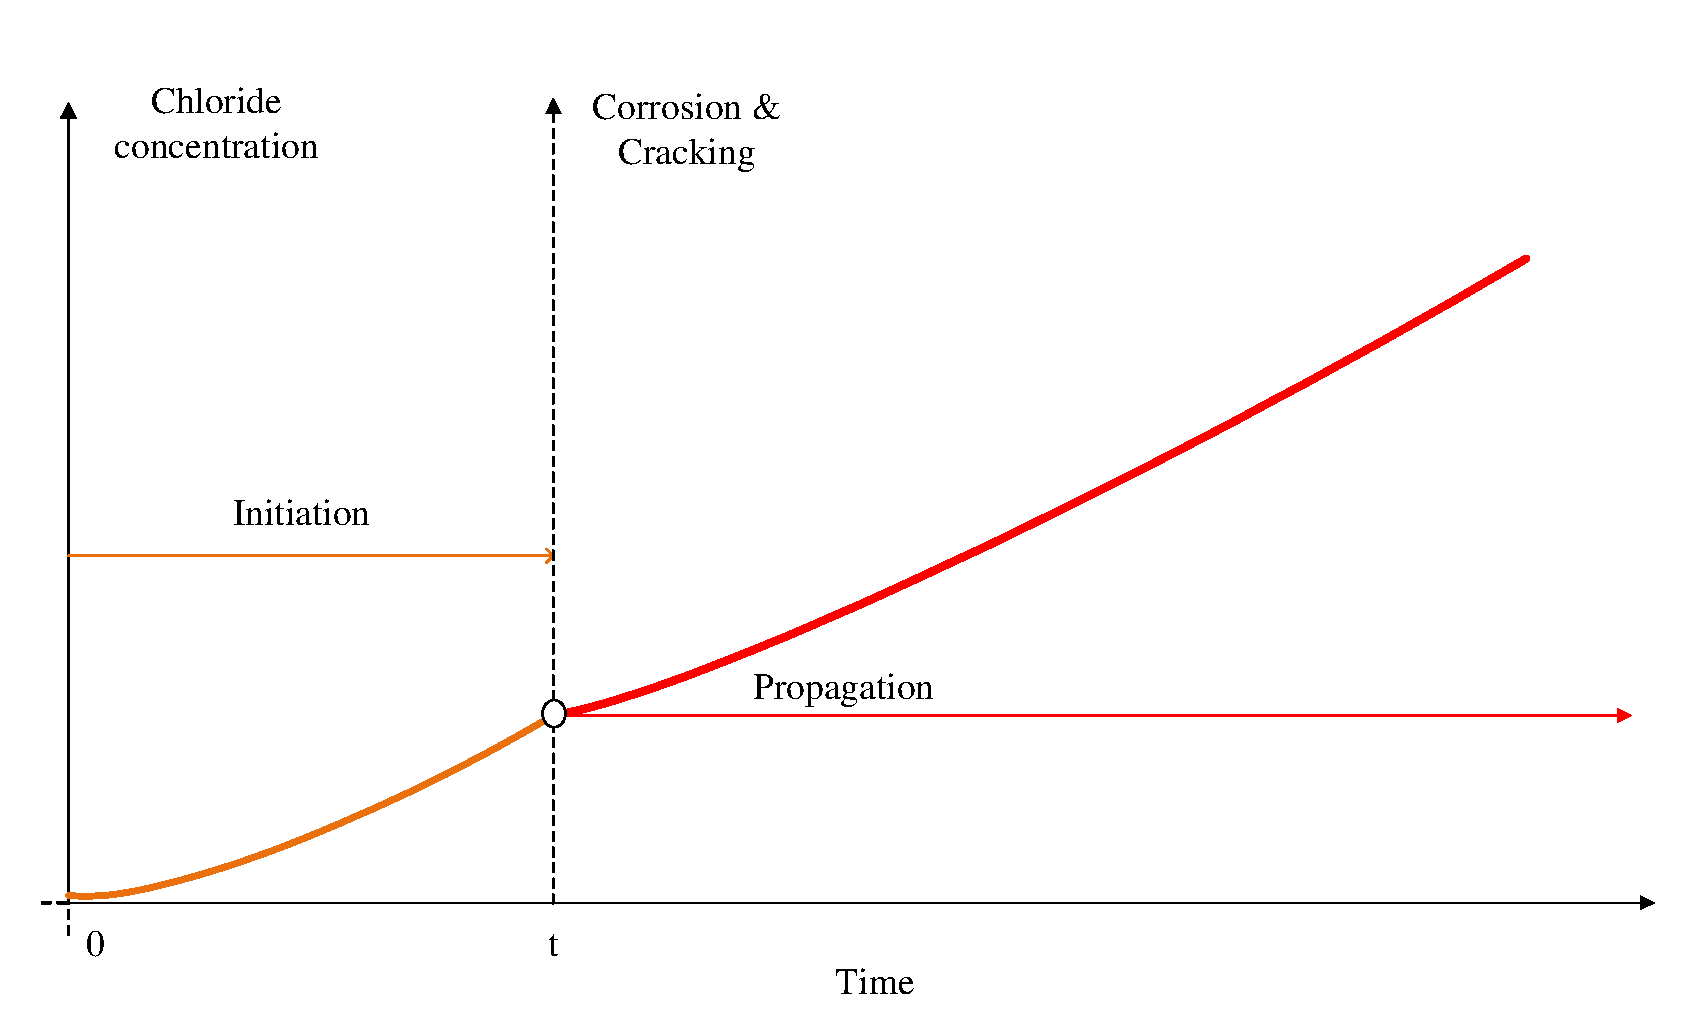
\includegraphics[width=300pt]{fig31.eps}
\caption{Deterioration process of reinforced concrete due to chloride-induced corrosion}\label{fig:31}
% \end{center}
\end{figure}
According to \cite{DuraCrete2000}, chloride penetration into reinforced concrete is a complicated process, which involves inter alia ion diffusion and convection \citep{Bertolini2013}. This complex transport mechanism can be represented by Fick's second law of diffusion.
\begin{eqnarray}
      && \frac{{\partial {C_{cl}}}}{{\partial t}} = {D_{cl}}\frac{{{\partial ^2}{C_{cl}}}}{{\partial x_{cl}^2}} \label{eq31}
\end{eqnarray}
Where:
\begin{adjustwidth}{1cm}{}
\begin{description}
\item[$C_{cl}$:] is the chloride ion concentration at the depth,
\item[$x_{cl}$:] from the surface of concrete after it exposes to chlorides till time \textit{t} (here small notation cl denotes the abbreviation for chloride).  
\item[$D_{cl}$:] is the chloride diffusion coefficient. 
\end{description}
%\end{flushright}
\end{adjustwidth}
The solution for partial differential equation of Eq. \eqref{eq31} gives the following explicit form to calculate the chloride concentration as a function of depth ${x_{cl}}$and time \textit{t}.
\begin{eqnarray}
      && {C_{cl}}({x_{cl}},t) = {C_s}\left( {1 - erf\left( {\frac{{{x_{cl}}}}{{2\sqrt {{D_{cl}}t} }}} \right)} \right) \label{eq32}
\end{eqnarray}
where  $erf\left(  \right)$denotes the error function\footnote{Definition of error function at http://en.wikipedia.org/wiki/Error\_function}. 

The duration for the diffusion process of chloride ion to initiate corrosion, that is time \textit{t} in Eq. \eqref{eq32}, can be estimated by setting the value of ${C_{cl}}$ to be equal to the chloride concentration. In other words, by setting the value of ${C_{cl}}$for each discrete condition state \textit{i}, the time to arrive at that CS can be obtained by solving Eq. \eqref{eq32} with respect to time \textit{t} and a certain depth of concrete cover from the re-bar.

For a bridge slab, value of variables ${C_{cl}}$,${C_s}$, and ${D_{cl}}$in the equation are can be considered as random, each one is associated with its own statistical distribution. Thus, estimation of time to arrive at certain value of chloride concentration is probabilistic in nature.

After the value of chloride concentration reaches a certain limit, corrosion starts on the reinforcing bars and after it reaches another higher limit the cracking process starts. The crack initiation phase is referred to here as the propagation phase and the width of the cracks over time can be determined by using following equations:
\begin{eqnarray}
      && w(t) = {w_0} + \beta  \cdot \left( {P(t) - {P_0}} \right) \label{eq33}
\end{eqnarray}
Where:
\begin{adjustwidth}{1cm}{}
\begin{description}
\item[$w(t)$:] width (mm) of crack over time,
\item[$\beta $:] the parameter that controls the propagation
\item[${w_0}$:] width of crack when it is visible (\textasciitilde{}0.05 mm)
\item[${P_0}$:] the amount of loss of re-bar diameter (mm) when crack width is visible 
\item [$P(t)$:] the amount of loss of re-bar diameter (mm) at \textit{t}
\end{description}
%\end{flushright}
\end{adjustwidth}

The reinforcement loss function can be represented as:
%
\begin{eqnarray}
      && P(t) = \int\limits_0^t {{V_{corr}} \cdot \alpha  \cdot wet \cdot tdt}  \label{eq34}
\end{eqnarray}
Where:
\begin{adjustwidth}{1cm}{}
\begin{description}
\item[${V_{corr}}$:] corrosion rate coefficient (mm/year)
\item[$wet$:] wet period in a year (equal to the ratio between total numbers of rainy day and 365 days)
\item[$\alpha $:] pitting factor that takes non-uniform corrosion of the re-bars into consideration
\end{description}
%\end{flushright}
\end{adjustwidth}

Based on field tests and experiments, statistical values of models coefficients and parameters are given in Table \ref{tbl:32}
% 
\begin{table}
\caption{Values of models parameters and coefficients}
\begin{tabular}{|l|l|l|l|l|l|}
\hline
\multicolumn{1}{|c|}{Parameters/ Coefficients} & \multicolumn{1}{c|}{Units} & Mean ($\mu$) & Standard deviation ($\sigma$) & Distribution & Reference equations \\ 
\hline
\multicolumn{1}{|c|}{$C_s$} & \multicolumn{1}{c|}{$wt.-\%Cl-/binder$} & \multicolumn{1}{c|}{2.565} & \multicolumn{1}{c|}{0.405} & \multicolumn{1}{c|}{Normal} & \multicolumn{1}{c|}{Eq. \eqref{eq32}} \\ 
\hline
\multicolumn{1}{|c|}{$x_{cl}$} & \multicolumn{1}{c|}{mm} & \multicolumn{1}{c|}{20} & \multicolumn{1}{c|}{NA} & \multicolumn{1}{c|}{NA} & \multicolumn{1}{c|}{Eq. \eqref{eq32}} \\ 
\hline
\multicolumn{1}{|c|}{$D_{cl}$} & \multicolumn{1}{c|}{NA} & \multicolumn{1}{c|}{100} & \multicolumn{1}{c|}{0.5} & \multicolumn{1}{c|}{Normal} & \multicolumn{1}{c|}{Eq. \eqref{eq32}} \\ 
\hline
\multicolumn{1}{|c|}{$w_0$} & \multicolumn{1}{c|}{mm} & \multicolumn{1}{c|}{0.05} & \multicolumn{1}{c|}{0.005} & \multicolumn{1}{c|}{Normal} & \multicolumn{1}{c|}{Eq. \eqref{eq33}} \\ 
\hline
\multicolumn{1}{|c|}{$P_0$} & \multicolumn{1}{c|}{mm} & \multicolumn{1}{c|}{5} & \multicolumn{1}{c|}{0.5} & \multicolumn{1}{c|}{Normal} & \multicolumn{1}{c|}{Eq. \eqref{eq33}} \\ 
\hline
\multicolumn{1}{|c|}{$\beta$} & \multicolumn{1}{c|}{NA} & \multicolumn{1}{c|}{0.001} & \multicolumn{1}{c|}{0.001} & \multicolumn{1}{c|}{Normal} & \multicolumn{1}{c|}{Eq. \eqref{eq33}} \\ 
\hline
\multicolumn{1}{|c|}{$V_{corr}$} & \multicolumn{1}{c|}{} & \multicolumn{1}{c|}{0.012} & \multicolumn{1}{c|}{0.006} & \multicolumn{1}{c|}{Normal} & \multicolumn{1}{c|}{Eq. \eqref{eq34}} \\ 
\hline
\multicolumn{1}{|c|}{$wet$} & \multicolumn{1}{c|}{year} & \multicolumn{1}{c|}{1} & \multicolumn{1}{c|}{0.25} & \multicolumn{1}{c|}{Normal} & \multicolumn{1}{c|}{Eq. \eqref{eq34}} \\ 
\hline
\multicolumn{1}{|c|}{$\alpha$} & \multicolumn{1}{c|}{NA} & \multicolumn{1}{c|}{14} & \multicolumn{1}{c|}{4.04} & \multicolumn{1}{c|}{Normal} & \multicolumn{1}{c|}{Eq. \eqref{eq34}} \\ 
\hline
\end{tabular}
\label{tbl:32}
\end{table}

\subsubsection{Question}
If you know that the chloride concentration ${C_{crit}}$ which starts the propagation phase is ${C_{cl}} = {C_{crit}} = 0.48$, and you consider that once a crack width is 0.5 mm, that an intervention is required to ensure that an adequate LOS is provided, when do you need to plan an intervention to ensure that an adequate LOS is provided? 

Hint: Construct a probabilistic deterioration model with discrete condition states for the entire chloride induced corrosion process of the bridge slab.
\subsubsection{Answer}
\paragraph{Condition states}
Since the deterioration process of chloride induced corrosion is a continuous process with two distinct phases, it is useful to define ranges of condition states for each phase in order to construct the probabilistic deterioration model with discrete condition states. This is illustrated in Figure \ref{fig:32}, when 5 condition states are used. Two are attributed to the initiation phase and two to the propagation phase.
\begin{figure}[h]
% \begin{center}
\includegraphics[width=300pt]{fig32.eps}
\caption{Deterioration process with discrete condition states}\label{fig:32}
% \end{center}
\end{figure}
In Figure \ref{fig:32}, five discrete condition states are used to illustrate the process. Their definitions are explained in Table \ref{tbl:33}.

\begin{table}
%	\centering
	\caption{Definition of condition states} \label{tbl:33}
		\begin{tabular}{|l|l|p{3.5cm}|p{5.5cm}|l|}
\hline
\multicolumn{1}{|c|}{Phase} & \multicolumn{1}{c|}{CS} & \multicolumn{1}{c|}{Description} & \multicolumn{1}{c|}{Indicator} & \multicolumn{1}{c|}{Criteria} \\ 
\hline
\multicolumn{1}{|c|}{1} & \multicolumn{1}{c|}{1} & New/partial new & Amount of chlorides in & \multicolumn{1}{c|}{$0 < C_{cl}\le 0.24$} \\ 
\cline{2-3}\cline{5-5}
\multicolumn{1}{|c|}{} & \multicolumn{1}{c|}{2} & Concrete contaminated & the concrete at reinforcing bar level $C_{cl}$ & \multicolumn{1}{c|}{$0.24 < C_{cl}\le 0.48$} \\ 
\hline
\multicolumn{1}{|c|}{2} & \multicolumn{1}{c|}{3} & Corrosion has initiated, no visible cracking has occurred & \multicolumn{1}{c|}{} & \multicolumn{1}{c|}{$C_{cl}> 0.48, w\le 0.25$} \\ 
\cline{2-3}\cline{5-5}
\multicolumn{1}{|c|}{} & \multicolumn{1}{c|}{4} & Visible cracking has occurred & Width of crack ($w$) & \multicolumn{1}{c|}{$0.25 < w \le 0.5$} \\ 
\cline{2-3}\cline{5-5}
\multicolumn{1}{|c|}{} & \multicolumn{1}{c|}{5} & Visible cracking has occurred and cover has spalled off & \multicolumn{1}{c|}{} & \multicolumn{1}{c|}{$ w > 0.5$} \\ 
\hline
\end{tabular}
\end{table}

\paragraph{Deterioration: Chloride concentration}

Using Eq. \eqref{eq32}, the concentration of chlorides at any time \textit{t} can be deterministically estimated given the mean values of the parameters of the model. These are, however, probabilistic in nature, thus, an explicit and straightforward arithmetic calculation is not always desirable. At any time in the future, for example, the value of ${C_{cl}}$ can be represented by using the mean and standard deviation. This concept is illustrated in Figure \ref{fig:33} for a normal distribution, where the mean value $\mu$ and standard deviation $\sigma$ are 0.3 and 0.08, respectively

\begin{figure}[h]
% \begin{center}
\includegraphics[width=300pt]{fig33.eps}
\caption{Probability of condition state CS 1-initiation phase.}\label{fig:33}
% \end{center}
\end{figure}
 
In order to determine when an intervention is required to ensure that an adequate LOS is provided, the probability of being in each condition state over time needs to be calculated.

Let assume that it is time \textit{t} now, and the probability of the bridge slab being in CS 1 will be equivalent to the probability that its continuous value falls between 0 and 0.24. The equation used to estimate the red area is.

In order to determine when an intervention is required to ensure that an adequate LOS is provided, the probability of being in each condition state over time needs to be calculated. 

Let assume that it is time t now, and the probability of the bridge slab being in $CS1$ will be equivalent to the probability that its continuous value falls between 0 and 0.24. The equation used to estimate the red area is.
\begin{eqnarray}
      && P_1 =P_1^{cl} = Prob[CS=1]=Prob[0 \leq C_{cl} \leq 0.24] = \int_0^{0.24}f(x) \cdot dx = 0.227 \label{stateprobcs1}
\end{eqnarray}
where $f(x)$ is density function of the normal distribution. 
\begin{eqnarray}
      && f(x)= \frac{1}{\sigma \sqrt{2\pi}}\cdot e^{-\frac{(x-\mu)^2}{2\sigma^2}}\label{densitynormaldistribu}
\end{eqnarray}
Similarly, the probability that the bridge element is in $CS2$ is given by:
\begin{eqnarray}
      && P_2 = P_2^{cl} = Prob[CS=2]=Prob[0.24 \leq C_{cl} \leq 0.48] \nonumber \\
      && = \int_{0.24}^{0.48}f(x) \cdot dx = 0.761 \label{stateprobcs2}
\end{eqnarray}
The probability that the bridge slab is in $CS3$ is in a condition state greater than CS2 is then given by:
\begin{eqnarray}
      && P_{>2} = P_{>2}^{cl} = 1-Prob[CS=2]-Prob[CS=2]=1-0.227-0.761=0.012\label{stateprobcs345}
\end{eqnarray}
%
\begin{figure}[h!]
% \centering
\includegraphics[width=300pt]{fig34.eps} 
\caption{Probability of condition state CS-2-initiation phase.} 
\label{fig:34}
\end{figure}
%
\paragraph{Deterioration: Corrosion propagation}

If it is assumed that the crack width can be modeled using a normal distribution with $\left[ {\mu  = 0.22,\sigma  = 0.03} \right]$ at time \textit{t} (the same time that is used to compute the state probability of the initiation phase), then the probability of being in condition state 3 is given by: 

\begin{figure}[h]
% \begin{center}
\includegraphics[width=300pt]{fig35.eps}
\caption{Probability of condition state CS 3-propagation phase.}
% \end{center}
\end{figure}

\begin{eqnarray}
      && P_3 = P_3^{cr} = Prob[CS=3]=Prob[w\leq0.25]\cdot Prob[C_{cl}>0.48] \nonumber \\
      && = 0.841 \cdot 0.012 = 0.010092\label{eq35}
\end{eqnarray}

Eq. \eqref{eq35} shows a joint probability of the event that chloride concentration level has reached more than its critical level 0.48 and corrosion has progressed to a point where at least one crack of 0.05 mm has opened up. The width of crack is, however, less than 0.25 mm.

Similarly, following state transition probabilities are obtained

\begin{eqnarray}
      && P_4 = P_4^{cr} = Prob[CS=4]=Prob[0.25 <w\leq0.5]\cdot Prob[C_{cl}>0.48] \nonumber \\
      && = 0.159 \cdot 0.012 = 0.001908\label{stateprobcs4} \\
      && P_5 = P_5^{cr} = Prob[CS=5]=Prob[w\geq 0.5]\cdot Prob[C_{cl}>0.48] = 0 \cdot 0.012 = 0 \label{stateprobcs5}
\end{eqnarray}

The above steps of calculation are used for a specific case when the condition state is defined in Table \ref{tbl:33}. For a general case that mathematically describes the relationship and for sake of programing, following generic formulation is used.

%
\begin{eqnarray}
&& {P_k} = \left\{ {\begin{array}{*{10}{c}}
{P_i^{cl} = \int\limits_a^b {f(x)dx} \hspace{0.2cm}i = (1,...,I){\rm{  }}}\\
{P_I^{cl} \cdot P_j^{cr} \hspace{1cm}   where \hspace{1cm} P_j^{cr} = \int\limits_c^d {g(x)dx} \hspace{1cm}j = (1,...,J)}
\end{array}{\rm{    }}} \right. \label{eq36}
\end{eqnarray}

Where:%k = (1,...,\left[ {I + J - 1} \right])
\begin{adjustwidth}{1cm}{}
\begin{description}
\item[$P_i^{cl}$:] is state probability of CS $i$ of the initiation phase with total number CS of $I$
\item[$P_j^{cl}$:] is state probability of CS $j$ of the propagation phase with total number CS of $J$
\item[$f(x)$ and $g(x)$:] are density function of the normal distribution for the initiation phase and propagation phase, respectively.
\end{description}
%\end{flushright}
\end{adjustwidth}
\paragraph{State distribution as proportional data}
Once the mechanistic-empirical equation, and the probabilistic distributions of each parameter to be used are known than the probable value of both chloride concentration and crack width can be generated by running many simulations, e.g. $20’000$. Once enough points are generated at the point of time to be investigated, either the probabilistic distribution that best fits these points can be determined and from this distribution the probability of the bridge slab being in a specific condition state can be estimated, or the probability of the bridge being in each condition state can be estimated directly from the number of data points, e.g. $10’000/20’000$ are in the specified range. 

In previous steps of calculation, the example is shown only for a specific time $t$ given the mean $\mu$ and the standard deviation $\sigma$ for each process. However, these values have to be estimated at each time step given the probabilistic distribution of models parameters. Results of estimation are the state probabilities over a pre-defined number of years. This pool of state probabilities is proportional data and state probabilities of the bridge in previous year is not related to the following year.

\paragraph{Deterioration prediction}

Once the mechanistic-empirical equation, and the probabilistic distributions of each parameter to be used are known than the probable value of both chloride concentration and crack width can be generated by running many simulations, e.g. 20'000. Once enough points are generated at the point of time to be investigated, either the probabilistic distribution that best fits these points can be determined and from this distribution the probability of the bridge slab being in a specific condition state can be estimated, or the probability of the bridge being in each condition state can be estimated directly from the number of data points, e.g. 10'000 / 20'000 are in the specified range. 

In previous steps of calculation, the example is shown only for a specific time \textit{t} given the mean $\mu$ and the standard deviation $\sigma$ for each process. However, these values have to be estimated at each time step given the probabilistic distribution of models parameters (Table \ref{tbl:32}).

Results of the estimation are the state probability over a pre-defined number of years. In this example, calculation is done for 60 years. At each year, the probabilistic value of chloride concentration ${C_{cl}}$ and the width of crack $X$ are re-computed using a pool of 20'000 samples that were randomly generated using Monte Carlo simulation. Then, the state probability that the bridge slab arrives at each discrete CS was computed for every year. These are shown in graphically in Figure \ref{fig:36}. 

\begin{figure}[h]
% \begin{center}
\includegraphics[width=324pt]{fig36.eps}
\caption{Condition state distribution over 60 years}\label{fig:36}
% \end{center}
\end{figure}
 
\paragraph{Results}

As can be seen from Figure \ref{fig:36}, in the first 7 years after the construction of the bridge slab, the chloride concentration is not expected to reach a value of 0.25. In other words, the bridge slab is expected to remain in CS 1. Then, the probability of the bridge slab being in CS 1 decreases, in the mean-time, of course, the probability that the bridge slab is in CS 2 increases. After 10 years, there is almost a 50\% chance that the bridge slab will be in CS 2.

Between the 7$^{th}$ and 10$^{th}$ years, there is a non-zero probability that the critical chloride concentration has been reached (0.48), i.e. the propagation phase has started. This explains the appearance of CS 3, CS 4 and CS 5 in the chart.

After 20 years, there is a high probability that the critical chloride concentration has been reached and the propagation phase has started. There is also approximately a 40\% chance that the surface of the slab will have at least one crack with a width between 0.00 mm and 0.25 mm. More or less the same chance that the crack width will be between 0.25 mm and 0.5 mm. There is, however, also a 20\% chance that the crack width will be greater than 0.5 mm, and that an intervention will have to be executed to ensure that an adequate LOS is provided.

So, since I know that the chloride concentration ${C_{crit}}$ that starts the propagation phase is ${C_{cl}} = {C_{crit}} = 0.48$, and if I consider that once a crack width is 0.5 mm that an intervention is required to ensure that an adequate LOS is provided, I will plan an intervention in year 15, when the probability of being in CS5 is still, according to my calculations is under 0.01 (Table \ref{tbl:34}). 
\begin{table}
%	\centering
	\caption{Evolution of state probability over 30 years} \label{tbl:34}
\begin{tabular}{|l|l|l|l|l|l|}
\hline
\multicolumn{1}{|m{1.5cm}|}{\centering year} & \multicolumn{5}{c|}{Condition states} \\ 
\cline{2-6}
\multicolumn{1}{|c|}{} & \multicolumn{1}{m{1.5cm}|}{\centering 1} & \multicolumn{1}{m{1.5cm}|}{\centering 2} & \multicolumn{1}{m{1.5cm}|}{\centering 3} & \multicolumn{1}{m{1.5cm}|}{\centering 4} & \multicolumn{1}{m{1.5cm}|}{\centering 5} \\ 
\hline
\multicolumn{1}{|c|}{1} & \multicolumn{1}{c|}{1} & \multicolumn{1}{c|}{0} & \multicolumn{1}{c|}{0} & \multicolumn{1}{c|}{0} & \multicolumn{1}{c|}{0} \\ 
\hline
\multicolumn{1}{|c|}{2} & \multicolumn{1}{c|}{1} & \multicolumn{1}{c|}{0} & \multicolumn{1}{c|}{0} & \multicolumn{1}{c|}{0} & \multicolumn{1}{c|}{0} \\ 
\hline
\multicolumn{1}{|c|}{3} & \multicolumn{1}{c|}{1} & \multicolumn{1}{c|}{0} & \multicolumn{1}{c|}{0} & \multicolumn{1}{c|}{0} & \multicolumn{1}{c|}{0} \\ 
\hline
\multicolumn{1}{|c|}{4} & \multicolumn{1}{c|}{1} & \multicolumn{1}{c|}{0} & \multicolumn{1}{c|}{0} & \multicolumn{1}{c|}{0} & \multicolumn{1}{c|}{0} \\ 
\hline
\multicolumn{1}{|c|}{5} & \multicolumn{1}{c|}{1} & \multicolumn{1}{c|}{0} & \multicolumn{1}{c|}{0} & \multicolumn{1}{c|}{0} & \multicolumn{1}{c|}{0} \\ 
\hline
\multicolumn{1}{|c|}{6} & \multicolumn{1}{c|}{1} & \multicolumn{1}{c|}{0} & \multicolumn{1}{c|}{0} & \multicolumn{1}{c|}{0} & \multicolumn{1}{c|}{0} \\ 
\hline
\multicolumn{1}{|c|}{7} & \multicolumn{1}{c|}{0.9174} & \multicolumn{1}{c|}{0.0826} & \multicolumn{1}{c|}{0} & \multicolumn{1}{c|}{0} & \multicolumn{1}{c|}{0} \\ 
\hline
\multicolumn{1}{|c|}{8} & \multicolumn{1}{c|}{0.5520} & \multicolumn{1}{c|}{0.3907} & \multicolumn{1}{c|}{0.0574} & \multicolumn{1}{c|}{0} & \multicolumn{1}{c|}{0} \\ 
\hline
\multicolumn{1}{|c|}{9} & \multicolumn{1}{c|}{0.2977} & \multicolumn{1}{c|}{0.3571} & \multicolumn{1}{c|}{0.3452} & \multicolumn{1}{c|}{0} & \multicolumn{1}{c|}{0} \\ 
\hline
\multicolumn{1}{|c|}{10} & \multicolumn{1}{c|}{0.1718} & \multicolumn{1}{c|}{0.2123} & \multicolumn{1}{c|}{0.6149} & \multicolumn{1}{c|}{0.001} & \multicolumn{1}{c|}{0} \\ 
\hline
\multicolumn{1}{|c|}{11} & \multicolumn{1}{c|}{0.1065} & \multicolumn{1}{c|}{0.1181} & \multicolumn{1}{c|}{0.7640} & \multicolumn{1}{c|}{0.0114} & \multicolumn{1}{c|}{0} \\ 
\hline
\multicolumn{1}{|c|}{12} & \multicolumn{1}{c|}{0.0693} & \multicolumn{1}{c|}{0.0672} & \multicolumn{1}{c|}{0.8153} & \multicolumn{1}{c|}{0.0482} & \multicolumn{1}{c|}{0} \\ 
\hline
\multicolumn{1}{|c|}{13} & \multicolumn{1}{c|}{0.0466} & \multicolumn{1}{c|}{0.0396} & \multicolumn{1}{c|}{0.7965} & \multicolumn{1}{c|}{0.1173} & \multicolumn{1}{c|}{0.0001} \\ 
\hline
\multicolumn{1}{|c|}{14} & \multicolumn{1}{c|}{0.0319} & \multicolumn{1}{c|}{0.0242} & \multicolumn{1}{c|}{0.7360} & \multicolumn{1}{c|}{0.2069} & \multicolumn{1}{c|}{0.0011} \\ 
\hline
\multicolumn{1}{|c|}{15} & \multicolumn{1}{c|}{0.0221} & \multicolumn{1}{c|}{0.0151} & \multicolumn{1}{c|}{0.6584} & \multicolumn{1}{c|}{0.2977} & \multicolumn{1}{c|}{0.0068} \\ 
\hline
\multicolumn{1}{|c|}{16} & \multicolumn{1}{c|}{0.0154} & \multicolumn{1}{c|}{0.0097} & \multicolumn{1}{c|}{0.5795} & \multicolumn{1}{c|}{0.3720} & \multicolumn{1}{c|}{0.0234} \\ 
\hline
\multicolumn{1}{|c|}{17} & \multicolumn{1}{c|}{0.0107} & \multicolumn{1}{c|}{0.0063} & \multicolumn{1}{c|}{0.5073} & \multicolumn{1}{c|}{0.4195} & \multicolumn{1}{c|}{0.0561} \\ 
\hline
\multicolumn{1}{|c|}{18} & \multicolumn{1}{c|}{0.0075} & \multicolumn{1}{c|}{0.0041} & \multicolumn{1}{c|}{0.4447} & \multicolumn{1}{c|}{0.4387} & \multicolumn{1}{c|}{0.1050} \\ 
\hline
\multicolumn{1}{|c|}{19} & \multicolumn{1}{c|}{0.0052} & \multicolumn{1}{c|}{0.0027} & \multicolumn{1}{c|}{0.3918} & \multicolumn{1}{c|}{0.4344} & \multicolumn{1}{c|}{0.1659} \\ 
\hline
\multicolumn{1}{|c|}{20} & \multicolumn{1}{c|}{0.0036} & \multicolumn{1}{c|}{0.0018} & \multicolumn{1}{c|}{0.3477} & \multicolumn{1}{c|}{0.4139} & \multicolumn{1}{c|}{0.2330} \\ 
\hline
\multicolumn{1}{|c|}{21} & \multicolumn{1}{c|}{0.0025} & \multicolumn{1}{c|}{0.0012} & \multicolumn{1}{c|}{0.3110} & \multicolumn{1}{c|}{0.3842} & \multicolumn{1}{c|}{0.3011} \\ 
\hline
\multicolumn{1}{|c|}{22} & \multicolumn{1}{c|}{0.0017} & \multicolumn{1}{c|}{0.0008} & \multicolumn{1}{c|}{0.2805} & \multicolumn{1}{c|}{0.3506} & \multicolumn{1}{c|}{0.3664} \\ 
\hline
\multicolumn{1}{|c|}{23} & \multicolumn{1}{c|}{0.0012} & \multicolumn{1}{c|}{0.0005} & \multicolumn{1}{c|}{0.2551} & \multicolumn{1}{c|}{0.3164} & \multicolumn{1}{c|}{0.4268} \\ 
\hline
\multicolumn{1}{|c|}{24} & \multicolumn{1}{c|}{0.0008} & \multicolumn{1}{c|}{0.0004} & \multicolumn{1}{c|}{0.2337} & \multicolumn{1}{c|}{0.2839} & \multicolumn{1}{c|}{0.4812} \\ 
\hline
\multicolumn{1}{|c|}{25} & \multicolumn{1}{c|}{0.0006} & \multicolumn{1}{c|}{0.0002} & \multicolumn{1}{c|}{0.2157} & \multicolumn{1}{c|}{0.2539} & \multicolumn{1}{c|}{0.5296} \\ 
\hline
\multicolumn{1}{|c|}{26} & \multicolumn{1}{c|}{0.0004} & \multicolumn{1}{c|}{0.0002} & \multicolumn{1}{c|}{0.2005} & \multicolumn{1}{c|}{0.2269} & \multicolumn{1}{c|}{0.5721} \\ 
\hline
\multicolumn{1}{|c|}{27} & \multicolumn{1}{c|}{0.0003} & \multicolumn{1}{c|}{0.0001} & \multicolumn{1}{c|}{0.1874} & \multicolumn{1}{c|}{0.2030} & \multicolumn{1}{c|}{0.6093} \\ 
\hline
\multicolumn{1}{|c|}{28} & \multicolumn{1}{c|}{0.0002} & \multicolumn{1}{c|}{0.0001} & \multicolumn{1}{c|}{0.1762} & \multicolumn{1}{c|}{0.1819} & \multicolumn{1}{c|}{0.6417} \\ 
\hline
\multicolumn{1}{|c|}{29} & \multicolumn{1}{c|}{0.0001} & \multicolumn{1}{c|}{0} & \multicolumn{1}{c|}{0.1664} & \multicolumn{1}{c|}{0.1634} & \multicolumn{1}{c|}{0.6700} \\ 
\hline
\multicolumn{1}{|c|}{30} & \multicolumn{1}{c|}{0.0001} & \multicolumn{1}{c|}{0} & \multicolumn{1}{c|}{0.1580} & \multicolumn{1}{c|}{0.1472} & \multicolumn{1}{c|}{0.6947} \\ 
\hline
\end{tabular}
\end{table}
As I know, however, that CS5 does not necessarily mean that an inadequate LOS is provided, I can also treat it as a warning that an inadequate LOS is coming if I don't do anything, but that I have a bit of time before this will happen. In this case, I may plan the intervention to be in year 20, when the probability of being in CS5 is 0.233. If I decide to wait until there is 50\% of being in CS5 than I will plan the intervention for either year 24 or 25. Whether or not this is a good decision depends on the probability of an inadequate LOS occurring once the slab reaches CS5 and the consequences if the adequate LOS happens, i.e. the risk associated with being in CS5.

The steps of numerical calculation can be tracked by reading the R script for this example provided at the Appendix \ref{mepi1}.
%
\section{Regression models} \label{regressionmodel}
\subsection{Theory}
Regression models represent empirical relationships between multiple parameters and are developed using regression analysis. They are used to predict the change in the value of a dependent variable based on the changes in the values of independent variables. Each variable is described in terms of its mean and variance. The simplest form is a linear regression model as shown in equation \ref{eq37}. Other forms are possible.

\begin{eqnarray}
 && {Y_i} = \alpha  + \beta  \cdot {X_i} + {\varepsilon _i} \label{eq37}
\end{eqnarray}
Where:
\begin{adjustwidth}{1cm}{}
\begin{description}
\item[${Y_i}$:] is the dependent variable or output (e.g. state probability of \textit{CS i}) that is observable
\item[${X_i}$:] is the characteristic or explanatory variable that is also observable (e.g. time, traffic volume, ambient temperature).
\item[$\alpha ,\beta $:] are parameters that need to be estimated.
\item[$\varepsilon $:] is the prediction error that can be assumed to follow a certain distribution (e.g. normal or log-normal distributions)
\end{description}
%\end{flushright}
\end{adjustwidth}

The mean or expected value of $Y_i$ for each value of input $X_i$ is
\begin{eqnarray}
 && E{Y_i} = \hat{\alpha}  + \hat{\beta}  \cdot {X_i} + {\varepsilon _i} \label{eq38}
\end{eqnarray}
The overhead mark ${\rm{\hat{\hspace{1mm}}}}$ indicates the expected values.

The purpose of performing a regression analysis is to predict the expected values of the regression parameters $\hat \alpha ,\hat \beta $ that minimize following objective function.
\begin{eqnarray}
 && s = {\sum\limits_{i = 1}^N {\left[ {{Y_i} - {{\hat Y}_i}} \right]} ^2} = {\sum\limits_{i = 1}^N {\left[ {{Y_i} - \hat \alpha  - \hat \beta  \cdot {X_i}} \right]} ^2} \label{eq39}
\end{eqnarray}

In words, the objective of Eq. \eqref{eq39} is to minimize the sum of the prediction errors. Here \textit{N} is the total of data points. 

In order to obtain the values of the regression parameters, one way of analytically solving Eq. \eqref{eq39} with respect to two variables $\hat \alpha ,\hat \beta $ (hereafter refer as a vector set $\hat \theta $). This can be done by taking the first derivative of Eq. \eqref{eq39} and set it to be equal to 0, and then solve for $\hat \theta $.
\begin{eqnarray}
 && \frac{{\partial s}}{{\partial \hat \theta }} = 0 \label{eq310}
\end{eqnarray}
For the value of $\hat \alpha $
\begin{manyeqns}
 && \frac{{\partial s}}{{\partial \hat \alpha }} = 0 \label{eq311} \\
 && \Leftrightarrow \frac{{{{\bar Y}^2} - 2 \cdot \bar Y(\hat \alpha  + \hat \beta  \cdot \bar X) + {{(\hat \alpha  + \hat \beta  \cdot \bar X)}^2}}}{{\partial \hat \alpha }} = 0\\
 && \Leftrightarrow  - 2 \cdot \bar Y + 2 \cdot \hat \alpha  + 2 \cdot \hat \beta  \cdot \bar X = 0\\
 && \Leftrightarrow \hat \alpha  = \bar Y - \hat \beta  \cdot \bar X
\end{manyeqns}
%
Here, the bar ${\rm{\bar{\hspace{1mm}}  }}$ indicates the value of $\frac{{\sum\limits_{i = 1}^N {{X_i}} }}{N}$ and $\frac{{\sum\limits_{i = 1}^N {{Y_i}} }}{N}$, which are the mean values.

Similarly, for the value of $\hat \beta $
\begin{manyeqns}
  && \frac{{\partial s}}{{\partial \hat \beta }} = 0\\
 && \Leftrightarrow \frac{{{{\bar Y}^2} - 2 \cdot \bar Y(\hat \alpha  + \hat \beta  \cdot \bar X) + {{(\hat \alpha  + \hat \beta  \cdot \bar X)}^2}}}{{\partial \hat \beta }} = 0\\
 && \Leftrightarrow \beta  \cdot \sum\limits_{i = 1}^N {X_i^2}  - \sum\limits_{i = 1}^N {{X_i} \cdot {Y_i}}  + \alpha \sum\limits_{i = 1}^N {{X_i}}  = 0\\
 && \Leftrightarrow \frac{{\sum\limits_{i = 1}^N {{X_i} \cdot {Y_i}}  - n \cdot \bar X \cdot \bar Y}}{{\sum\limits_{i = 1}^N {X_i^2 - n \cdot \bar X} }} = \frac{{\sum\limits_{i = 1}^N {({X_i} - \bar X) \cdot ({Y_i} - \bar Y)} }}{{\sum\limits_{i = 1}^N {{{({X_i} - \bar X)}^2}} }}
\end{manyeqns}
Following figure graphically represents the regression equation and the calculation.

\begin{figure}[h]
% \begin{center}
\includegraphics[width=300pt]{fig37.eps}
\caption{Deriving linear regression coefficients}
% \end{center}
\end{figure}

The goodness of fit of the regression line can be measured by the coefficient ${R^2}$, which measures the proportion of total variation about the mean $\bar Y$, which is explained by regression:
\begin{eqnarray}
 && {R^2} = \frac{{\sum\limits_{i = 1}^N {{{({{\hat Y}_i} - \bar Y)}^2}} }}{{\sum\limits_{i = 1}^N {{{({Y_i} - \bar Y)}^2}} }} = \frac{{{\beta ^2} \cdot \sum\limits_{i = 1}^N {{{({X_i} - \bar X)}^2}} }}{{\sum\limits_{i = 1}^N {{{({{\hat Y}_i} - \bar Y)}^2}} }} \label{eq321}
\end{eqnarray}
The prediction errors can be followed an independent type of distribution. In many practical situation, normal distribution is often used. In case of normal distribution $N(\mu ,\sigma )$, its mean and standard deviation are defined as:
\begin{eqnarray}
 && {\mu _\varepsilon } = {Y_i} - {\hat Y_i} \label{eq322}\\
 && {\sigma _\varepsilon } = \sqrt {\frac{{\sum\limits_{i = 1}^N {{{({Y_i} - {Y_i})}^2}} }}{{N - k - 1}}}
\end{eqnarray}
Where \textit{k} is number of independent variable, which is equal to 1 in this example (as there is only one input X).

The above example is for the case of simple linear regression with only one independent variable. In many practical situations, linear regression models can be built for multiple variables, which often takes following form.
\begin{eqnarray}
 && Y = \sum\limits_{i = 0}^N {\beta _{}^k}  \cdot X_i^k \label{eq3223}
\end{eqnarray}
Where $k = 1,...,K$ is a vector set of numbers of independent variables. 
\subsection{Example}
Assuming that you have many reinforced concrete slabs, as the one discussed in section 2.2 and have measured chloride concentrations and crack widths over the years, you may have the plots shown in Figure \ref{fig:38} and Figure \ref{fig:39}\footnote{Data used for this example is selected from the pool of randomly generated total data used in the previous example, taking into consideration of the mean and standard deviation at each time t.}. (This data will be distributed in a .csv file in addition to this text).
\begin{figure}[h]
%\begin{center}
\includegraphics[width=300pt]{fig38.eps}
\caption{Measured chloride concentrations in similar deck slabs over time}\label{fig:38}
%\end{center}
\end{figure}
\begin{figure}[h]
%\begin{center}
\includegraphics[width=300pt]{fig39.eps}
\caption{Measured crack widths in similar deck slabs over time}\label{fig:39}
%\end{center}
\end{figure}
\subsubsection{Question}
If you know that the chloride concentration ${C_{crit}}$ which starts the propagation phase is ${C_{cl}} = {C_{crit}} = 0.48$, as in the previous example, and you consider that the once a crack width of 0.5 mm is reached, that an intervention is required to ensure that an adequate LOS is provided, when do you need to plan an intervention to ensure that an adequate LOS is provided? (Use linear regression analysis with the values of chloride concentration and crack width provided, estimate the functional form of deterioration).
\subsubsection{Answer}
As deterioration of the bridge slab is seen as happening in two different phases, separate models are developed using regression analysis for both phases; one for the initiation phase with chloride concentration and other for the propagation phase with the development of crack.
\paragraph{Condition states}
The condition states are defined exactly as in Table \ref{tbl:33}.
\paragraph{Deterioration: Chloride concentration} \label{chrloride}
The form of regression equation for chloride concentration, when it is assumed to be linear is:
\begin{eqnarray}
 && Y_i^{cl} = {\alpha _{cl}} + {\beta _{cl}} \cdot X_i^{cl} + \varepsilon _i^{cl} \label{eq3224}
\end{eqnarray}
Where:
\begin{adjustwidth}{1cm}{}
\begin{description}
\item[$Y_i^{cl}$:] is the value of chloride concentration at year \textit{i}.
\item[$X_i^{cl}$:] is the year \textit{i}.
\item[${\alpha _{cl}},{\beta _{cl}}$:] are regression parameters that need to be estimated.
\item[$\varepsilon _i^{cl}$:] is the prediction errors following a normal distribution
\end{description}
%\end{flushright}
\end{adjustwidth}
The expected values of regression parameters can be obtained using the R code in the Appendix \ref{mepi3} on data created using the Appendix \ref{mepi2}. The results are in listing \ref{mechaempichlorine}.

\lstinputlisting[basicstyle=\ttfamily\scriptsize,float=h,frame=tb,caption=Results-Chloride concentration,label=mechaempichlorine]{./Programs/IMP-mecha-empi/IMP-chloridecon.tex}

The value of the regression parameters are: ${\alpha _{cl}} =  - 3.40275$ and ${\beta _{cl}} = 0.47975$. The value of ${R^2}$ is greater than 0.8959, which is nearly 10\% far from 1. This means that the fitness of the linear model to this data set infers a small variation. This can also be seen from Figure \ref{fig:310}, which shows fitted line of chloride concentration at the surface of the reinforcement as time goes by.
\begin{figure}[h]
% \begin{center}
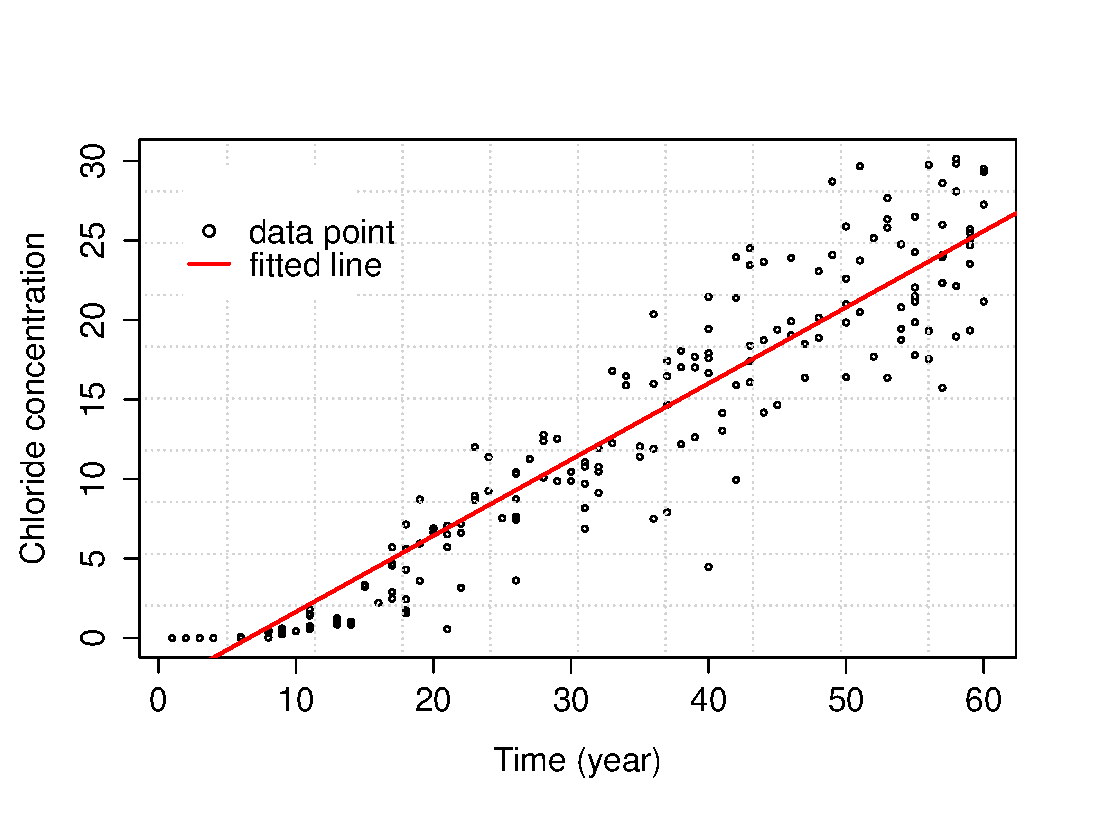
\includegraphics[width=304pt]{fig310.eps}
\caption{Development of chloride concentration}\label{fig:310}
% \end{center}
\end{figure}
The equation to be used for estimating the chloride concentration over time is then

\begin{eqnarray}
 && Y_i^{cl} =  - 3.40275 + 0.47975 \cdot X_i^{cl} \label{eq3225}
\end{eqnarray}
Noted that the value of chloride concentration cannot be negative, therefore, it is necessary to consider a dummy variable to control the results of calculation
\begin{eqnarray}
 && Y_i^{cl} = ( - 3.40275 + 0.47975 \cdot X_i^{cl}) \cdot \delta _i^{cl} \label{eq3226}\\
 && where{\rm{\hspace{2mm} }}\delta _i^{cl} = \left\{ {\begin{array}{*{20}{c}}
{0{\rm{\hspace{2mm}   when \hspace{2mm} X}}_i^{cl} < 7}\\
{1{\rm{\hspace{2mm}   when \hspace{2mm}  X}}_i^{cl} \ge 7{\rm{ }}}
\end{array}} \right.
\end{eqnarray}
Where 7 is the integer value closest to the ratio 3.40275/0.4975. An integer value is used here as the years are used as discrete units of time. 

This result is obtained by running the R code provided in the Appendix \ref{mepi3} on data created using the Appendix \ref{mepi2}.
%
\paragraph{Deterioration: Crack propagation}
To estimate the development of crack width using a regression model, a step similar to the one in section \ref{chrloride} is used. Following results (listing \ref{mechaempicrack}) are obtained (using the R code provided in the Appendix \ref{mepi3}).

\lstinputlisting[basicstyle=\ttfamily\scriptsize,float=h,frame=tb,caption=Results-Crack,label=mechaempicrack]{./Programs/IMP-mecha-empi/IMP-crackpropa.tex}

\begin{figure}[h]
% \begin{center}
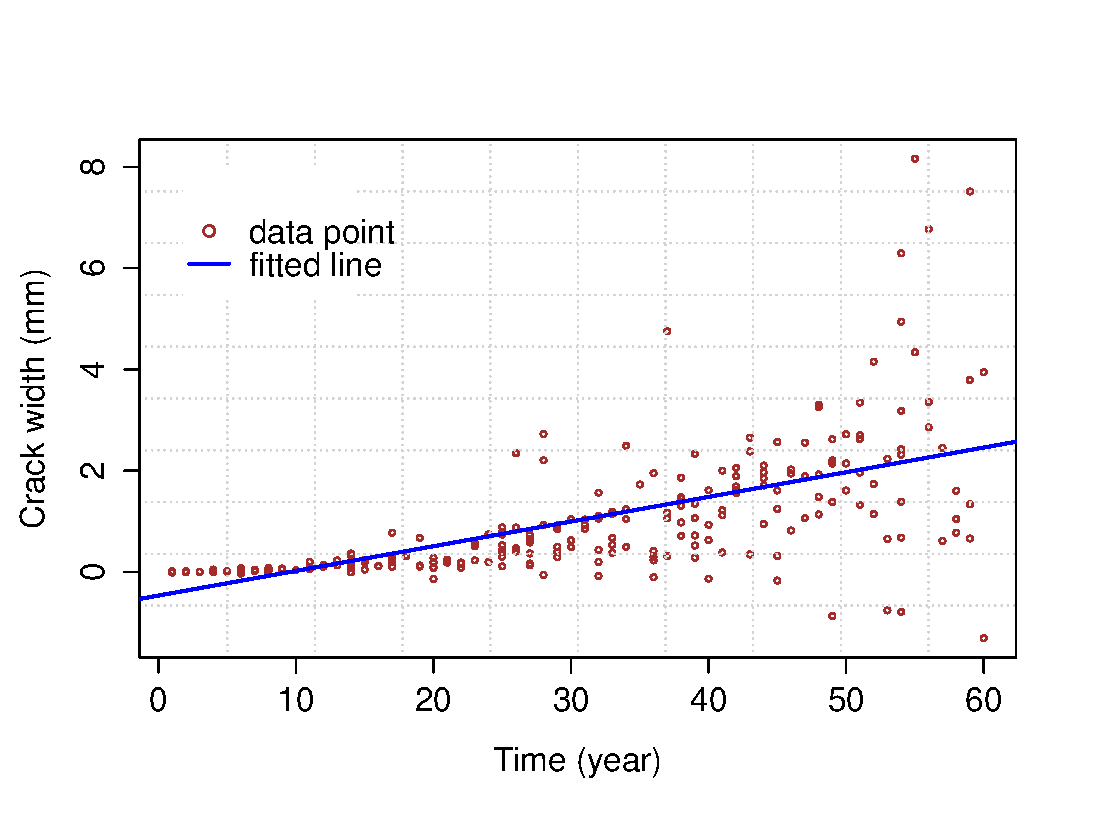
\includegraphics[width=305pt]{fig311.eps}
\caption{Development of crack width}
\label{fig:311}
% \end{center}
\end{figure}
The equation to be used to predict crack width is then:
\begin{eqnarray}
 && Y_i^{cr} = ( - 0.500755 + 0.053150 \cdot X_i^{cr}) \cdot \delta _i^{cr} \label{eq3227}\\
 && where{\rm{\hspace{2mm} }}\delta _i^{cr} = \left\{ {\begin{array}{*{20}{c}}
{0{\rm{ \hspace{2mm}  when \hspace{2mm} X}}_i^{cr} < 9}\\
{1{\rm{ \hspace{2mm}  when \hspace{2mm}  X}}_i^{cr} \ge 9{\rm{ }}}
\end{array}} \right.
\end{eqnarray}
Where 9 is the integer value closest to the ratio 0.500755/0.053150. An integer value is used here as the years are used as discrete units of time.
%
\paragraph{Deterioration prediction}

Using the regression equations given above, the predicted deterioration is as shown in Figure \ref{fig:312}. The curve consists of three pieces. The first piece represents the period of time from new construction until the chloride concentration at the reinforcement level is thought to be equivalent to that determined by the regression equation. The second piece represents the period of time where the chloride concentration at the reinforcement can be represented by the regression equation to the point where corrosion has started to an extent to cause at least one crack wider than 0.5 mm, and the third piece shows the propagation phase, i.e. the extension of cracking once at least one crack is wider than 0.5 mm. This is represented by the second regression equation.
\begin{figure}[h]
% \begin{center}
\includegraphics[width=305pt]{fig312.eps}
\caption{Development of crack width}
 \label{fig:312}
% \end{center}
\end{figure}
\paragraph{Results}
As can be seen from the deterioration curve estimated by using regression model, by the time of 17 years, the chloride concentration certainly reach to a level that higher than 0.48. It means the bridge slab will enter CS 3 and the second phase of deterioration will start, which initiates cracking. Since the time to the worst condition state (CS 5) from the time propagation phase starts will be about 10 years, meaning that the total duration of deterioration from CS1 to CS 5 is about 27 years.

So, since I know that the chloride concentration ${C_{crit}}$ that starts the propagation phase is ${C_{cl}} = {C_{crit}} = 0.48$, and if I consider that once a crack width is 0.5 mm that an intervention is required to ensure that an adequate LOS is provided, I will plan an intervention before year 27. 
\section{Comparison mechanistic-empirical models vs. regression models}
Using both models, and planning an intervention when there is a 50\% chance that the bridge slab will be in CS5 are the same (27 years). 

Using the mechanistic model, in the way we did we could also determine the probability of the bridge slab being in CS5 in each time interval through-out the investigated time period. This made it possible to set other criteria on when to intervene, e.g. the probability of being in CS5 is negligible, or less than 20\%. This was not possible using the regression model the way we did. If it was desired to take into consideration risk, using the regression analysis one would need to arbitrarily pick an earlier point in time to plan the intervention, e.g. in year 20 and not in year 25. 

The use of the mechanistic-empirical model requires a lot of information on the specific values of the parameters to be used in the model, estimates of the uncertainty of the model, and the model. It is suitable in situations where there is not a lot of data on the performance of the deck slabs, and it is feasible to estimate the distributions to be used to represent the values of the parameters, develop the model, and estimate model uncertainty.

The use of the regression model requires a lot of information on the performance of similar deck slabs. It is suitable in situations where this information exists.
\section{Assignments}
\subsection{Problem A - Erosion of concrete cover of waste water tanks}
In a waste water treatment plant, reinforced concrete tanks are used to store the waste water before going through the cleaning process. Waste water is stored in the tanks and various chemical substances are poured into the tanks for the purposes of disinfection. The cement deteriorates due to this exposure. 

The infrastructure manager is interested in predicting the condition of the tanks so that the maintenance interventions can be better planned over the next 30 years. She realizes that these can be estimated using the results of past inspections performed at 2 years intervals (Table \ref{tbl:35}). The first inspection time was executed 1 year after the begin use of the tanks. It is a general rule of thumb that the erosion should not be more than 12 mm.
%
\begin{table}
%	\centering
	\caption{Inspection data} \label{tbl:35}
\begin{tabular}{|l|l|l|l|l|l|}
\hline
\multicolumn{1}{|c|}{Tank} & \multicolumn{5}{c|}{Depth of erosion (m)} \\ 
\cline{2-6}
\multicolumn{1}{|c|}{} & \multicolumn{1}{c|}{inspection 1} & \multicolumn{1}{c|}{inspection 2} & \multicolumn{1}{c|}{inspection 3} & \multicolumn{1}{c|}{inspection 4} & \multicolumn{1}{c|}{inspection 5} \\ 
\hline
\multicolumn{1}{|c|}{1} & \multicolumn{1}{c|}{0.2} & \multicolumn{1}{c|}{1.1} & \multicolumn{1}{c|}{2.4} & \multicolumn{1}{c|}{3.8} & \multicolumn{1}{c|}{4.9} \\ 
\hline
\multicolumn{1}{|c|}{2} & \multicolumn{1}{c|}{0.5} & \multicolumn{1}{c|}{0.9} & \multicolumn{1}{c|}{1.7} & \multicolumn{1}{c|}{3.5} & \multicolumn{1}{c|}{5.2} \\ 
\hline
\multicolumn{1}{|c|}{3} & \multicolumn{1}{c|}{2} & \multicolumn{1}{c|}{2.7} & \multicolumn{1}{c|}{3.2} & \multicolumn{1}{c|}{4.5} & \multicolumn{1}{c|}{5.5} \\ 
\hline
\multicolumn{1}{|c|}{4} & \multicolumn{1}{c|}{1.5} & \multicolumn{1}{c|}{3.1} & \multicolumn{1}{c|}{3.6} & \multicolumn{1}{c|}{5.5} & \multicolumn{1}{c|}{6.3} \\ 
\hline
\multicolumn{1}{|c|}{5} & \multicolumn{1}{c|}{1.1} & \multicolumn{1}{c|}{1.8} & \multicolumn{1}{c|}{1.9} & \multicolumn{1}{c|}{3.1} & \multicolumn{1}{c|}{4.9} \\ 
\hline
\multicolumn{1}{|c|}{6} & \multicolumn{1}{c|}{0.7} & \multicolumn{1}{c|}{1.5} & \multicolumn{1}{c|}{2} & \multicolumn{1}{c|}{3.8} & \multicolumn{1}{c|}{5.1} \\ 
\hline
\multicolumn{1}{|c|}{7} & \multicolumn{1}{c|}{0.8} & \multicolumn{1}{c|}{0.9} & \multicolumn{1}{c|}{1.8} & \multicolumn{1}{c|}{4.2} & \multicolumn{1}{c|}{5.4} \\ 
\hline
\multicolumn{1}{|c|}{8} & \multicolumn{1}{c|}{1} & \multicolumn{1}{c|}{1.9} & \multicolumn{1}{c|}{2.6} & \multicolumn{1}{c|}{3.9} & \multicolumn{1}{c|}{5} \\ 
\hline
\multicolumn{1}{|c|}{9} & \multicolumn{1}{c|}{0.9} & \multicolumn{1}{c|}{1.7} & \multicolumn{1}{c|}{3.6} & \multicolumn{1}{c|}{4.3} & \multicolumn{1}{c|}{7.1} \\ 
\hline
\multicolumn{1}{|c|}{10} & \multicolumn{1}{c|}{0.8} & \multicolumn{1}{c|}{0.9} & \multicolumn{1}{c|}{1.6} & \multicolumn{1}{c|}{4.1} & \multicolumn{1}{c|}{6.7} \\ 
\hline
\multicolumn{1}{|c|}{11} & \multicolumn{1}{c|}{0.5} & \multicolumn{1}{c|}{1.8} & \multicolumn{1}{c|}{2.3} & \multicolumn{1}{c|}{3.7} & \multicolumn{1}{c|}{5.8} \\ 
\hline
\multicolumn{1}{|c|}{12} & \multicolumn{1}{c|}{0.6} & \multicolumn{1}{c|}{1.2} & \multicolumn{1}{c|}{2.2} & \multicolumn{1}{c|}{3.6} & \multicolumn{1}{c|}{6} \\ 
\hline
\end{tabular}
\end{table}

She also realizes that this can be done using by constructing and testing tank walls in the laboratory. After having done this her engineers have come up with the following mechanistic deterioration model.
\begin{eqnarray}
 && f(t + 1) = f(t) \cdot {e^\beta }\label{eq3228}
\end{eqnarray}
Where:
\begin{adjustwidth}{1cm}{}
\begin{description}
\item[$f(t+1)$:] is the depth of corrosion.
\item[$\beta$:] is the deterioration coefficient taking its value of 0.1.
\end{description}
%\end{flushright}
\end{adjustwidth}
It is assumed that $f(0) = 0$ and $f(1) = 1$\footnote{This assumption is used to prevent the value of function $f$ to be equal to 0 at year t=0}.

\subsection{Question A1}
What is the condition of each object in 30 years if the mechanistic-empirical model is used?
\subsection{Question A2}
What is the condition of each object in 30 years if predictions are made using a regression analysis?
\subsection{Answer A1}
Using Eq. \eqref{eq3228}, the evolution of erosion over 30 years is shown in Table \ref{tbl:36} and Figure \ref{fig:313}. 

\begin{table}
%	\centering
	\caption{Evolution of erosion (mechanistic-empirical model)} \label{tbl:36}
\begin{tabular}{|l|l|l|l|l|l|}
\hline
\multicolumn{1}{|c|}{Time} & \multicolumn{1}{c|}{Erosion} & \multicolumn{1}{c|}{Time} & \multicolumn{1}{c|}{Erosion} & \multicolumn{1}{c|}{Time} & \multicolumn{1}{c|}{Erosion} \\ 
\multicolumn{1}{|c|}{(years)} & \multicolumn{1}{c|}{(mm)} & \multicolumn{1}{c|}{(years)} & \multicolumn{1}{c|}{(mm)} & \multicolumn{1}{c|}{(years)} & \multicolumn{1}{c|}{(mm)} \\ 
\hline
\multicolumn{1}{|c|}{1} & \multicolumn{1}{c|}{1} & \multicolumn{1}{c|}{11} & \multicolumn{1}{c|}{2.7183} & \multicolumn{1}{c|}{21} & \multicolumn{1}{c|}{7.3891} \\ 
\hline
\multicolumn{1}{|c|}{2} & \multicolumn{1}{c|}{1.1052} & \multicolumn{1}{c|}{12} & \multicolumn{1}{c|}{3.0042} & \multicolumn{1}{c|}{22} & \multicolumn{1}{c|}{8.1662} \\ 
\hline
\multicolumn{1}{|c|}{3} & \multicolumn{1}{c|}{1.2214} & \multicolumn{1}{c|}{13} & \multicolumn{1}{c|}{3.3201} & \multicolumn{1}{c|}{23} & \multicolumn{1}{c|}{9.0250} \\ 
\hline
\multicolumn{1}{|c|}{4} & \multicolumn{1}{c|}{1.3499} & \multicolumn{1}{c|}{14} & \multicolumn{1}{c|}{3.6693} & \multicolumn{1}{c|}{24} & \multicolumn{1}{c|}{9.9742} \\ 
\hline
\multicolumn{1}{|c|}{5} & \multicolumn{1}{c|}{1.4918} & \multicolumn{1}{c|}{15} & \multicolumn{1}{c|}{4.0552} & \multicolumn{1}{c|}{25} & \multicolumn{1}{c|}{11.0232} \\ 
\hline
\multicolumn{1}{|c|}{6} & \multicolumn{1}{c|}{1.6487} & \multicolumn{1}{c|}{16} & \multicolumn{1}{c|}{4.4817} & \multicolumn{1}{c|}{26} & \multicolumn{1}{c|}{12.1825} \\ 
\hline
\multicolumn{1}{|c|}{7} & \multicolumn{1}{c|}{1.8221} & \multicolumn{1}{c|}{17} & \multicolumn{1}{c|}{4.9530} & \multicolumn{1}{c|}{27} & \multicolumn{1}{c|}{13.4637} \\ 
\hline
\multicolumn{1}{|c|}{8} & \multicolumn{1}{c|}{2.0138} & \multicolumn{1}{c|}{18} & \multicolumn{1}{c|}{5.4739} & \multicolumn{1}{c|}{28} & \multicolumn{1}{c|}{14.8797} \\ 
\hline
\multicolumn{1}{|c|}{9} & \multicolumn{1}{c|}{2.2255} & \multicolumn{1}{c|}{19} & \multicolumn{1}{c|}{6.0496} & \multicolumn{1}{c|}{29} & \multicolumn{1}{c|}{16.4446} \\ 
\hline
\multicolumn{1}{|c|}{10} & \multicolumn{1}{c|}{2.4596} & \multicolumn{1}{c|}{20} & \multicolumn{1}{c|}{6.6859} & \multicolumn{1}{c|}{30} & \multicolumn{1}{c|}{18.1741} \\ 
\hline
\end{tabular}
\end{table}

\begin{figure}[h]
% \begin{center}
\includegraphics[width=300pt]{fig313.eps}
\caption{Evolution of erosion – mechanistic-empirical model}
 \label{fig:313}
% \end{center}
\end{figure}
%
By the year 26, if the infrastructure manager has not already executed an intervention, the depth of erosion will reach 12 mm, which is beyond the critical level. In order to prevent the re-bars of tanks from the onset of corrosion, an intervention (e.g. renewal of cover layer of the tanks walls) should be executed before year 26. 
\subsection{Answer A2}
Assuming that the form of the regression is linear, the general regression equation is:
\begin{eqnarray}
 && Y_i^{ero} = {\alpha _{ero}} + {\beta _{ero}} \cdot X_i^{ero} + \varepsilon _i^{ero} \label{eq3229}
\end{eqnarray}
Where:
\begin{adjustwidth}{1cm}{}
\begin{description}
\item[$Y_i^{ero}$:] is the value of erosion at year \textit{i}.
\item[$X_i^{ero}$:] is the year \textit{i}.
\item[${\alpha _{ero}},{\beta _{ero}}$:] are regression parameters that need to be estimated.
\item[$\varepsilon _i^{ero}$:] is the prediction errors following a normal distribution
\end{description}
%\end{flushright}
\end{adjustwidth}
Using the linear regression analysis (refer to section \ref{regressionmodel}), and in the Appendix \ref{mepi4}, following results are obtained (listing \ref{mechaempiwaste}).

\lstinputlisting[basicstyle=\ttfamily\scriptsize,float=h,frame=tb,caption=Results,label=mechaempiwaste]{./Programs/IMP-mecha-empi/IMP-A-waste-water-tanks.tex}

\begin{eqnarray}
 && Y_i^{ero} =  - 0.03630 + 0.59171 \cdot X_i^{ero} \label{eq3230}
\end{eqnarray}
\begin{figure}[h]
% \begin{center}
\includegraphics[width=302pt]{fig314.eps}
\caption{Evolution of erosion - linear regression model}\label{fig:314}
% \end{center}
\end{figure}
 
The fitted line plotted from Eq. \eqref{eq3230} is shown in Figure \ref{fig:314}. When the level of erosion becomes 12 mm, it corresponds to 20 years. If the infrastructure manager relies solely on this analysis she will plan the intervention to be executed before year 20.
\subsection{Problem B - Bridge wear out}
An infrastructure manager wants to make a work program for a bridge, i.e. when an intervention needs to be executed and what type of intervention. He normally models deterioration using the following mechanistic-empirical model:
\begin{eqnarray}
 && I = \exp (\lambda  \cdot t) - 1 \label{eq3231}
\end{eqnarray}
Where is $\lambda $is the deterioration coefficient, which is given by:
\begin{eqnarray}
 && \lambda  = \frac{{\ln (2)}}{{Tc}} \label{eq3232}
\end{eqnarray}
In Eq. \eqref{eq3231}, $Tc$ represents the average life time of the structure elements of the bridge. It is modeled using a normal distribution with mean and standard deviation equal to 60 years and 7 years, respectively. A detail description of the model can be referred to the work of \cite{Brodsky2006}. The manager divides condition into five discrete states given in Table \ref{tbl:37}. The wear out of the bridge has its value from 0 to 1 as defined in Eq. \eqref{eq3232}.
\begin{table}
%	\centering
	\caption{Definition of condition states} \label{tbl:37}
\begin{tabular}{|l|l|l|}
\hline
\multicolumn{1}{|c|}{Condition states} & \multicolumn{1}{c|}{Description} & \multicolumn{1}{c|}{Corresponding values of I} \\ 
\hline
\multicolumn{1}{|c|}{1} & \multicolumn{1}{c|}{New/Partially new} & \multicolumn{1}{c|}{$I<0.2$} \\ 
\hline
\multicolumn{1}{|c|}{2} & \multicolumn{1}{c|}{Good} & \multicolumn{1}{c|}{$0.2\le I <0.4$} \\ 
\hline
\multicolumn{1}{|c|}{3} & \multicolumn{1}{c|}{Average} & \multicolumn{1}{c|}{$0.4\le I <0.6$} \\ 
\hline
\multicolumn{1}{|c|}{4} & \multicolumn{1}{c|}{Bad} & \multicolumn{1}{c|}{$0.6\le I <0.8$} \\ 
\hline
\multicolumn{1}{|c|}{5} & \multicolumn{1}{c|}{Very bad} & \multicolumn{1}{c|}{$I\ge0.8$}\\
\hline
\end{tabular}
\end{table}
\subsection{Question}
What is the probabilistic distribution of discrete condition states over the next 50 years for the bridge? What does this mean?

\subsection{Answer}
As the value of $Tc$ is probabilistic in nature, the value of I is also probabilistic. A Monte Carlo simulation with 20'000 iterations is used to estimate the probability of \textit{I} having values that correspond with each of the condition states over time. The results are shown in Figure \ref{fig:315}. The R code in the Appendix \ref{mepi5} is used to estimate the probability of the bridge being in each condition state over 50 years. 
\begin{figure}[h]
% \begin{center}
\includegraphics[width=300pt]{fig315.eps}
\caption{Condition state distribution over 50 years}\label{fig:315}
% \end{center}
\end{figure}
As can be seen from the figure, in the first 10 years after the construction of the bridge, the bridge will remains in CS1. Then, the probability that the bridge is in CS1 decreases and the probability that it will be in CS2 increases. After 30 years, there is a 50\% probability that the bridge will be in CS2.

After 30 years, there is a small probability that the bridge will be in CS3, and after 40 years, a 50\% probability that the bridge will be in CS 4. The speed of degradation increases rapidly after 30 years. By year 50, the probability that the bridge is in CS 5 is more than 50\%. 

Based on this information the infrastructure manager might consider executing an intervention before year 40 to avoid an inadequate LOS from occurring. The steps of numerical calculation can be tracked by reading the R script for this example provided at the the Appendix \ref{mepi5}.

%
\bibliographystyle{plainnat}
\bibliography{reference}
\pagebreak

\begin{subappendices}
% \label{appendix3}
% \label{appendix3}
\section{R code for the mechanistic-empirical model-concrete bridge slab}\label{mepi1}
% \textbf{R code for the mechanistic-empirical model-concrete bridge slab}
\lstinputlisting[basicstyle=\ttfamily\scriptsize]{./Programs/IMP-mecha-empi/IMP-Mechanistic-Emprical-model.r}
\pagebreak
\section{R code for generating data}\label{mepi2}
% \textbf{R code for generating data}
\lstinputlisting[basicstyle=\ttfamily\scriptsize]{./Programs/IMP-mecha-empi/IMP-data-generation.r}
\pagebreak
\section{R code for regression analysis} \label{mepi3}
% \textbf{R code for regression analysis}
\lstinputlisting[basicstyle=\ttfamily\scriptsize]{./Programs/IMP-mecha-empi/IMP-regression.r}
\pagebreak
\section{R code for estimation of erosion evolution over 30 years} \label{mepi4}
% \textbf{R code for estimation of erosion evolution over 30 years}
\lstinputlisting[basicstyle=\ttfamily\scriptsize]{./Programs/IMP-mecha-empi/IMP-A-waste-water-tanks.r}
\pagebreak
\section{R code for chloride concentration} \label{mepi5}
% \textbf{R code for chloride concentration}
\lstinputlisting[basicstyle=\ttfamily\scriptsize]{./Programs/IMP-mecha-empi/IMP-A-bridge-wear-out.r}
\end{subappendices}
% \pagebreak
% \section*{Appendix 3.4} \label{mepi4}
% \textbf{R code for regression analysis}
% \lstinputlisting{./Programs/IMP-chapter3-R/IMP-4-regression.r}

 
 
 
 
 
 
 
%%%%%%%%%%%%%%%%%%%%% chapter.tex %%%%%%%%%%%%%%%%%%%%%%%%%%%%%%%%%
%
% sample chapter
%
% Use this file as a template for your own input.
%
%%%%%%%%%%%%%%%%%%%%%%%% Springer-Verlag %%%%%%%%%%%%%%%%%%%%%%%%%%
%\motto{Use the template \emph{chapter.tex} to style the various elements of your chapter content.}
\chapter{Event Tree and Fault Tree Analysis}
\label{faulteventreechapter} % Always give a unique label
% use \chaptermark{}
% to alter or adjust the chapter heading in the running head
\chapterauthor{Bryan T. Adey and Nam Lethanh}
\section{Event tree analysis - Theory}
\subsection{Definition}
Event tree analysis (ETA) is a way to analyse and display different discrete
scenarios, their corresponding probability of occurrence and the resulting
consequences. ETA uses Boolean logic to analyse a chronological sequence of
events and estimate the probability of their occurrence. A key component of event
tree analysis is the event tree. An event tree is built from a starting event and
branches at each subsequent event based on the values of key parameters these key
parameters were intensity measures. When the event tree is complete, it is a
logical and visual representation of the set of scenarios that can occur, i.e.
multiple possible futures. An example is shown in Figure \ref{figeventfault:1}, the
initiating event is a 100-year precipitation, which may result in the occurrence
of a flood with water depths over 30 cm, under 30 cm, or not at all. In this
example, the flood can lead to different damage states related to an
infrastructure element, which can result in interruptions to traffic flow on the
road network. The consequences of the scenarios can then be quantified. Also the
heavy rain itself can cause an interruption.
\begin{figure}[h]
% \begin{center}
\includegraphics[width=300pt]{faulteventtree-1.eps}
\caption{Simplified event tree for a flood risk analysis}\label{figeventfault:1}
% \end{center}
\end{figure}
ETA is often referred to as having forward logic as it starts from an initiating
event and ends at a consequence. It is often used to analyze the risks associated
with systems, and the consequences of functioning or failed systems given that an
event(s) has (have) occurred. Simply the construction of an event tree can often
be useful in decision situations as it brings to light many scenarios that
decision makers otherwise would not have considered.

When conducting an ETA it is necessary to first determine the starting events
that are to be considered and then to think through each of the next possible
events to be considered. Each chain of events from initiating events to the end
event (or consequence) is referred to as a path, and may be thought of as a
scenario.

At each node in the event tree, the tree branches. There are often only two
branches that emanate from a node but it is possible that no split occurs or that
many splits occur. It is, however, of utmost importance to ensure that the split
represents mutually exclusive possibilities, i.e. if one possibility happens the
other cannot happen. The end events are often referred to as consequences.

The construction of an event tree requires knowledge about the system.
\subsection{Steps}


The basic steps to conduct an event tree analysis are:
\begin{enumerate}
\item Define static system: Determine what you would like to model and what is not to
be considered in the model
\item Define dynamic system: Determine what you would like to model over time. For
example, what hazards are of particular concern, e.g. flooding, what physical
things may happen, e.g. bridge collapse, what consequences might occur, e.g.
horrendous increases in travel times due to traffic jams
\item Identify specific initiating events: For example, heavy rain fall.
\item Identify specific intermediate events: For example, overtopping of a bridge
\item Construct the event tree
\item Calculate the probabilities of occurrence of each event: One possibility is
using fault tree analysis.
\item Calculate the probability of occurrence of each scenario or path:
\item Calculate the overall risk:
\item Evaluate the acceptability of the risk associated with each scenario and
overall:
\end{enumerate}
%
Due to the almost infinite number of ways to represent reality and the almost
infinite number of events that can occur, an appropriate system representation
needs to be developed. A good starting point is often the system representation
used to determine that there was a problem. It needs, however, to be verified
that this representation is adequate for the evaluation of the candidate
strategies. The necessary detail to be used depends on the specific question, the
strategies to be evaluated and the level of detail desired.
\subsection{Example in literature}
Please read the research work of \cite{Beim1997}, who constructed a event
tree analysis for a lock gate system, as part of the script.
\section{Event tree analysis - Example}
\subsection{Question A}
You are the road manager responsible for a particularly risky section of road.
It consists of a bridge that crosses a river and is just below a steep
embankment, upon which it is known that avalanches sometimes occur. This is
illustrated in Figure \ref{figfaultevent2x}.
%
\begin{figure}
 \begin{minipage}[h]{0.5\linewidth}
        \centering
        \includegraphics[scale=0.95]{faulteventtree-31.eps}
				\subcaption{Flood event}\label{faulteventtree-31}
     \end{minipage}
\vspace{3.00mm}
    \begin{minipage}[h]{0.5\linewidth}
       \centering
       \includegraphics[scale=0.95]{faulteventtree-32.eps}
			\subcaption{Avalanche event}\label{faulteventtree-32}
     \end{minipage}
\caption{Illustration of risks}
\label{figfaultevent2x}
\end{figure}
%
You suspect that there are substantial infrastructure related risks due to both
flooding and avalanches but would like to quantify the risks. Develop an event
tree to allow you to do this.
\subsection{Answer A}
One of the first things to do when developing an event tree to allow you to
estimate the infrastructure related risks due to flooding and avalanches is to
determine the what will cause the branching in the event tree\footnote{The answer
is an adapted version of that used in \cite{Adey2009}}. The event tree is a part of the system
representation\footnote{The system representation is a model of the relevant part
of reality used for the evaluation and consists of all possible realizations of
stochastic processes within the investigated time period.}. The event tree in
this case should have sufficiently good representations of the structures,
hazards, and consequences, as well as the interaction between them so that it can
be reasonably certain that there is an appropriate understanding of the system
and that the risks. The event tree should consist of all possible things that can
happen in a specified period of time, i.e. scenarios. In the event tree a
scenario is represented by a path in the event tree. In the event tree proposed
here the paths are divided into five components, 1) event occurrence, 2) effect
of event, 3) physical changes in infrastructure, 4) direct consequences, and 5)
indirect consequences. An example for a bridge exposed to flooding and avalanches
is shown in Figure \ref{figeventfault:3}, assuming that flood and avalanche events are
mutually exclusive.
\begin{figure}[h]
\begin{center}
\includegraphics[width=300pt]{faulteventtree-13.eps}
\caption{Event tree with mutually exclusive flood and avalanche
events.}\label{figeventfault:3}
\end{center}
\end{figure}
In this event tree the hazard consists of the event and the effects on the
bridge object that are considered to have consequences. The effects on the bridge
are represented by two levels of the key parameters, water depth \textit{$>$= a
}and water depth \textit{$<$ a}, where \textit{a }is the bridge clearance, and
snow depth \textit{$>$= b }and snow depth \textit{$<$ b}, where \textit{b }is the
depth of snow on the bridge.

The consequence portion of the event tree is composed of the non-monetarisable
and monetarisable direct and indirect consequences. For each level of the key
parameter, assumptions are made with respect to the non-monetarisable direct
consequences that can occur, e.g. the physical behavior of the structure when the
specified level of the key parameter(s) occurs. The effect on the structure
should be described with the fewest possible parameters. Assumptions are made
with respect to the monetarisable direct consequences that can occur for each
non-monetarisable direct consequence, e.g. the fatalities related to the collapse
of the bridge. Assumptions are made with respect to the monetarisable indirect
consequences that can occur for each monetarisable direct consequence, e.g. the
additional user traffic time due to a deviation. The monetarisable consequences
can be attributed to those that will carry the consequences if failure occurs and
can be grouped by consequences type.
In the event tree (Figure \ref{figeventfault:3}), each effect has two possible
non-monetarisable direct consequences (\textit{nmDC{\tiny 1}, nmDC{\tiny 2}}).
For example, when the water depth during a flood is \textit{$>$= a}, than the two
possible failure modes are the wash out of the abutments (\textit{nmDC{\tiny 1}})
and the wash out of the columns (\textit{nmDC{\tiny 2}}). The monetarisable
direct consequences deterministically follow the non monetarisable direct
consequences (\textit{nmDC{\tiny 1}}). The monetarisable indirect consequences
are branched into the monetarisable indirect consequences that would occur if the
abutments were washed out during winter with low traffic volumes
(\textit{mIC{\tiny 1}}) and those that would occur if the abutments were washed
out during summer with high traffic volumes (\textit{mIC{\tiny 2}})
\subsection{Question B}
Construct an event tree for a road segment and a bridge that may be affected by
a flood or an avalanche, but not at the same time.
\subsection{Answer B}
The branches in the event tree are comprised of a chain of possible events and
monetarisable direct and indirect consequences (Fig. \ref{figeventfault:3} and Fig. \ref{figeventfault:4}). A slightly more
detailed example of some of the avalanche scenarios is given in Table
\ref{tbleventfault:1}, where the effect on the physical object is listed simply as level.
It is easy to imagine how detailed this can become.
\begin{figure}[h]
\begin{center}
\includegraphics[width=300pt]{faulteventtree-14.eps}
\caption{Event tree with mutually exclusive flood event.}\label{figeventfault:3}
\end{center}
\end{figure}

\begin{figure}[h]
\begin{center}
\includegraphics[width=300pt]{faulteventtree-15.eps}
\caption{Event tree with mutually exclusive avalanche event.}
\label{figeventfault:4}
\end{center}
\end{figure}

\begin{table}
	\centering
	\caption{Examples of scenarios} \label{tbleventfault:1}
\begin{tabular}{|c|c|c|c|}
\hline
Nr. & Effect & Non-monetarisable direct consequences & Monetarisable direct consequences \\ 
\hline
1 &  & Mild deformation of road surface & Level 1 \\ 
\cline{1-1}\cline{4-4}
2 &  &  & Level 2 \\ 
\cline{1-1}\cline{3-4}
3 &  & Severe deformation of road surface & Level 1 \\ 
\cline{1-1}\cline{4-4}
4 & On column level 1 &  & Level 2 \\ 
\cline{1-1}\cline{3-4}
5 &  & Collapse of object & Level 2 \\ 
\cline{1-1}\cline{4-4}
6 &  &  & Level 3 \\ 
\hline
- & - & - & - \\ 
- & - & - & - \\ 
- & - & - & - \\ 
\hline
31 &  & Mild displacement of deck & Level 1 \\ 
\cline{1-1}\cline{4-4}
32 &  &  & Level 2 \\ 
\cline{1-1}\cline{3-4}
33 &  & Severe displacement of deck & Level 1 \\ 
\cline{1-1}\cline{4-4}
34 & Horizontal loading of deck level 3 &  & Level 2 \\ 
\cline{1-1}\cline{3-4}
35 &  & Removal of superstructure & Level 2 \\ 
\cline{1-1}\cline{4-4}
36 &  &  & Level 3 \\ 
\hline
\end{tabular}
\end{table}
\subsection{Question C}
As a road manager you are considering the construction of avalanche protection
to reduce the infrastructure related risk.

You know that with respect to the probabilities of occurrence of events that
\begin{itemize}
\item if you do nothing,the probability of occurrence of an avalanche decreases from
0.5 in 2009 to 0.3 in 2029 due to ever decreasing snow fall.
\item If you construct avalanche protection, the probability of occurence of an
avalanche will be 0 for the next 10 years but will increase after that
\end{itemize}
You know that the conditional probabilities of the effects on the loading of the
column, the horizontal loading of the superstructure and the vertical loading of
the superstructure are constant and as shown in Table \ref{tbleventfault:2}. You know that
conditional probability of physical changes due to horizontal loading of the
columns and deck increases by 0.001 per year to take into account normal
deterioration (Table \ref{tbleventfault:3} and Table \ref{tbleventfault:4}) and due to vertical
loading of deck is 1 and constant (Table \ref{tbleventfault:5}). You also know that the due
to changes in traffic that the conditional probabilities of consequences are as
shown in Table \ref{tbleventfault:6}. You have also estimate the consequences of each
consequence level to be those as shown in Table \ref{tbleventfault:7}.

Is it worth it if only a 20 year horizon is analysed?  (Use a discount factor of
2\%. Assume that the probability of multiple failures of the same infrastructure
object are negligible. Show the yearly costs and benefits as well as the totals.
For simplicity, assume that there is only one level of monetarisable consequences
per level of physical damage.)

\begin{table}
	\centering
	\caption{Conditional probabilities of the effects} \label{tbleventfault:2}
\begin{tabular}{|l|l|l|l|l|l|l|l|l|l|}
\hline
\multicolumn{1}{|c|}{Year} & \multicolumn{3}{c|}{Loading of the column} & \multicolumn{3}{m{2.5cm}|}{\centering Horizontal loading of the superstructure} & \multicolumn{3}{m{2.5cm}|}{\centering Vertical loading of the superstructure} \\ 
\cline{2-10}
\multicolumn{1}{|c|}{} & \multicolumn{1}{c|}{Level 1} & \multicolumn{1}{c|}{Level 2} & \multicolumn{1}{c|}{Level 3} & \multicolumn{1}{c|}{Level 1} & \multicolumn{1}{c|}{Level 2} & \multicolumn{1}{c|}{Level 3} & \multicolumn{1}{c|}{Level 1} & \multicolumn{1}{c|}{Level 2} & \multicolumn{1}{c|}{Level 3} \\ 
\hline
\multicolumn{1}{|c|}{2009} & \multicolumn{1}{c|}{0.3} & \multicolumn{1}{c|}{0.4} & \multicolumn{1}{c|}{0.3} & \multicolumn{1}{c|}{0.3} & \multicolumn{1}{c|}{0.4} & \multicolumn{1}{c|}{0.3} & \multicolumn{1}{c|}{0.3} & \multicolumn{1}{c|}{0.4} & \multicolumn{1}{c|}{0.3} \\ 
\hline
\multicolumn{1}{|c|}{2010} & \multicolumn{1}{c|}{0.3} & \multicolumn{1}{c|}{0.4} & \multicolumn{1}{c|}{0.3} & \multicolumn{1}{c|}{0.3} & \multicolumn{1}{c|}{0.4} & \multicolumn{1}{c|}{0.3} & \multicolumn{1}{c|}{0.3} & \multicolumn{1}{c|}{0.4} & \multicolumn{1}{c|}{0.3} \\ 
\hline
\multicolumn{1}{|c|}{2011} & \multicolumn{1}{c|}{0.3} & \multicolumn{1}{c|}{0.4} & \multicolumn{1}{c|}{0.3} & \multicolumn{1}{c|}{0.3} & \multicolumn{1}{c|}{0.4} & \multicolumn{1}{c|}{0.3} & \multicolumn{1}{c|}{0.3} & \multicolumn{1}{c|}{0.4} & \multicolumn{1}{c|}{0.3} \\ 
\hline
\multicolumn{1}{|c|}{2012} & \multicolumn{1}{c|}{0.3} & \multicolumn{1}{c|}{0.4} & \multicolumn{1}{c|}{0.3} & \multicolumn{1}{c|}{0.3} & \multicolumn{1}{c|}{0.4} & \multicolumn{1}{c|}{0.3} & \multicolumn{1}{c|}{0.3} & \multicolumn{1}{c|}{0.4} & \multicolumn{1}{c|}{0.3} \\ 
\hline
\multicolumn{1}{|c|}{2013} & \multicolumn{1}{c|}{0.3} & \multicolumn{1}{c|}{0.4} & \multicolumn{1}{c|}{0.3} & \multicolumn{1}{c|}{0.3} & \multicolumn{1}{c|}{0.4} & \multicolumn{1}{c|}{0.3} & \multicolumn{1}{c|}{0.3} & \multicolumn{1}{c|}{0.4} & \multicolumn{1}{c|}{0.3} \\ 
\hline
\multicolumn{1}{|c}{-} & \multicolumn{1}{c}{-} & \multicolumn{1}{c}{-} & \multicolumn{1}{c}{-} & \multicolumn{1}{c}{-} & \multicolumn{1}{c}{-} & \multicolumn{1}{c}{-} & \multicolumn{1}{c}{-} & \multicolumn{1}{c}{-} & \multicolumn{1}{c|}{-} \\ 
\multicolumn{1}{|c}{-} & \multicolumn{1}{c}{-} & \multicolumn{1}{c}{-} & \multicolumn{1}{c}{-} & \multicolumn{1}{c}{-} & \multicolumn{1}{c}{-} & \multicolumn{1}{c}{-} & \multicolumn{1}{c}{-} & \multicolumn{1}{c}{-} & \multicolumn{1}{c|}{-} \\ 
\hline
\multicolumn{1}{|c|}{2025} & \multicolumn{1}{c|}{0.3} & \multicolumn{1}{c|}{0.4} & \multicolumn{1}{c|}{0.3} & \multicolumn{1}{c|}{0.3} & \multicolumn{1}{c|}{0.4} & \multicolumn{1}{c|}{0.3} & \multicolumn{1}{c|}{0.3} & \multicolumn{1}{c|}{0.4} & \multicolumn{1}{c|}{0.3} \\ 
\hline
\multicolumn{1}{|c|}{2026} & \multicolumn{1}{c|}{0.3} & \multicolumn{1}{c|}{0.4} & \multicolumn{1}{c|}{0.3} & \multicolumn{1}{c|}{0.3} & \multicolumn{1}{c|}{0.4} & \multicolumn{1}{c|}{0.3} & \multicolumn{1}{c|}{0.3} & \multicolumn{1}{c|}{0.4} & \multicolumn{1}{c|}{0.3} \\ 
\hline
\multicolumn{1}{|c|}{2027} & \multicolumn{1}{c|}{0.3} & \multicolumn{1}{c|}{0.4} & \multicolumn{1}{c|}{0.3} & \multicolumn{1}{c|}{0.3} & \multicolumn{1}{c|}{0.4} & \multicolumn{1}{c|}{0.3} & \multicolumn{1}{c|}{0.3} & \multicolumn{1}{c|}{0.4} & \multicolumn{1}{c|}{0.3} \\ 
\hline
\multicolumn{1}{|c|}{2028} & \multicolumn{1}{c|}{0.3} & \multicolumn{1}{c|}{0.4} & \multicolumn{1}{c|}{0.3} & \multicolumn{1}{c|}{0.3} & \multicolumn{1}{c|}{0.4} & \multicolumn{1}{c|}{0.3} & \multicolumn{1}{c|}{0.3} & \multicolumn{1}{c|}{0.4} & \multicolumn{1}{c|}{0.3} \\ 
\hline
\multicolumn{1}{|c|}{2029} & \multicolumn{1}{c|}{0.3} & \multicolumn{1}{c|}{0.4} & \multicolumn{1}{c|}{0.3} & \multicolumn{1}{c|}{0.3} & \multicolumn{1}{c|}{0.4} & \multicolumn{1}{c|}{0.3} & \multicolumn{1}{c|}{0.3} & \multicolumn{1}{c|}{0.4} & \multicolumn{1}{c|}{0.3} \\ 
\hline
\end{tabular}
\end{table}

\begin{table}
	\centering
	\caption{Conditional probabilities of the occurrence of the physical changes due to loading of the column} \label{tbleventfault:3}
\begin{tabular}{|c|c|c|c|}
\hline
Year & \multicolumn{3}{c|}{Effect} \\ 
\cline{2-4}
 & \multicolumn{3}{c|}{Loading of column} \\ 
\cline{2-4}
 & Mild deformation of road surface & Severe deformation of road surface & Collapse of object \\ 
\hline
2009 & 0.2 & 0.2 & 0.2 \\ 
\hline
2010 & 0.201 & 0.201 & 0.201 \\ 
\hline
2011 & 0.202 & 0.202 & 0.202 \\ 
\hline
2012 & 0.203 & 0.203 & 0.203 \\ 
\hline
- & - & - & - \\ 
- & - & - & - \\ 
\hline
2027 & 0.218 & 0.218 & 0.218 \\ 
\hline
2028 & 0.219 & 0.219 & 0.219 \\ 
\hline
2029 & 0.220 & 0.220 & 0.220 \\ 
\hline
\end{tabular}
\end{table}

\begin{table}
	\centering
	\caption{Conditional probabilities of the occurrence of the physical changes due to horizontal loading of the deck} \label{tbleventfault:4}
\begin{tabular}{|c|c|c|c|}
\hline
Year & \multicolumn{3}{c|}{Effect} \\ 
\cline{2-4}
 & \multicolumn{3}{c|}{Horizontal loading of deck} \\ 
\cline{2-4}
 & Mild deformation of road surface & Severe deformation of road surface & Collapse of object \\ 
\hline
2009 & 0.2 & 0.2 & 0.2 \\ 
\hline
2010 & 0.201 & 0.201 & 0.201 \\ 
\hline
2011 & 0.202 & 0.202 & 0.202 \\ 
\hline
2012 & 0.203 & 0.203 & 0.203 \\ 
\hline
- & - & - & - \\ 
- & - & - & - \\ 
\hline
2027 & 0.218 & 0.218 & 0.218 \\ 
\hline
2028 & 0.219 & 0.219 & 0.219 \\ 
\hline
2029 & 0.220 & 0.220 & 0.220 \\ 
\hline
\end{tabular}
\end{table}

\begin{table}
	\centering
	\caption{Conditional probabilities of the occurrence of the physical changes due to vertical loading of the deck} \label{tbleventfault:5}
\begin{tabular}{|c|c|c|c|}
\hline
Year & \multicolumn{3}{c|}{Effect} \\ 
\cline{2-4}
 & \multicolumn{3}{c|}{Vertical loading of deck} \\ 
\cline{2-4}
 & Slightly yielded reinforcement & Plasticized reinforcement & Collapse of object \\ 
\hline
2009 & 1 & 1 & 1 \\ 
\hline
2010 & 1 & 1 & 1 \\ 
\hline
2011 & 1 & 1 & 1 \\ 
\hline
2012 & 1 & 1 & 1 \\ 
\hline
- & - & - & - \\ 
- & - & - & - \\ 
\hline
2027 & 1 & 1 & 1 \\ 
\hline
2028 & 1 & 1 & 1 \\ 
\hline
2029 & 1 & 1 & 1 \\ 
\hline
\end{tabular}
\end{table}

\begin{table}
	\centering
	\caption{Conditional probabilities of monetarisable (direct and indirect) consequences} \label{tbleventfault:6}
\begin{tabular}{|l|l|l|l|l|l|l|l|l|}
\hline
\multicolumn{1}{|c|}{Year} & \multicolumn{4}{m{4.5cm}|}{\centering Loading of column (L1, L2, L3) Horizonal loading of deck} & \multicolumn{2}{m{2cm}|}{\centering Vertical loading of deck (L1, L2)} & \multicolumn{2}{m{2cm}|}{\centering Vertical load of deck (L3)} \\ 
\cline{2-9}
\multicolumn{1}{|c|}{} & \multicolumn{8}{c|}{Failure mode} \\ 
\cline{2-9}
\multicolumn{1}{|c|}{} & \multicolumn{2}{m{2cm}|}{\centering Deformation of road surface} & \multicolumn{2}{m{2cm}|}{\centering Collapse of object} & \multicolumn{2}{m{2cm}|}{\centering Slightly yielded / plastized rebar} & \multicolumn{2}{m{2cm}|}{\centering Collapse of object} \\ 
\cline{2-9}
\multicolumn{1}{|c|}{} & \multicolumn{8}{c|}{Monetarisable direct and indirect consequences} \\ 
\cline{2-9}
\multicolumn{1}{|c|}{} & \multicolumn{1}{c|}{Level 1} & \multicolumn{1}{c|}{Level 2} & \multicolumn{1}{c|}{Level 1} & \multicolumn{1}{c|}{Level 2} & \multicolumn{1}{c|}{Level 1} & \multicolumn{1}{c|}{Level 2} & \multicolumn{1}{c|}{Level 2} & \multicolumn{1}{c|}{Level 3} \\ 
\hline
\multicolumn{1}{|c|}{2009} & \multicolumn{1}{c|}{0.5} & \multicolumn{1}{c|}{0.5} & \multicolumn{1}{c|}{0.5} & \multicolumn{1}{c|}{0.5} & \multicolumn{1}{c|}{0.5} & \multicolumn{1}{c|}{0.5} & \multicolumn{1}{c|}{0.5} & \multicolumn{1}{c|}{0.5} \\ 
\hline
\multicolumn{1}{|c|}{2010} & \multicolumn{1}{c|}{0.499} & \multicolumn{1}{c|}{0.501} & \multicolumn{1}{c|}{0.499} & \multicolumn{1}{c|}{0.501} & \multicolumn{1}{c|}{0.499} & \multicolumn{1}{c|}{0.501} & \multicolumn{1}{c|}{0.499} & \multicolumn{1}{c|}{0.501} \\ 
\hline
\multicolumn{1}{|c|}{2011} & \multicolumn{1}{c|}{0.498} & \multicolumn{1}{c|}{0.502} & \multicolumn{1}{c|}{0.498} & \multicolumn{1}{c|}{0.502} & \multicolumn{1}{c|}{0.498} & \multicolumn{1}{c|}{0.502} & \multicolumn{1}{c|}{0.498} & \multicolumn{1}{c|}{0.502} \\ 
\hline
\multicolumn{1}{|c}{-} & \multicolumn{1}{c}{-} & \multicolumn{1}{c}{-} & \multicolumn{1}{c}{-} & \multicolumn{1}{c}{-} & \multicolumn{1}{c}{-} & \multicolumn{1}{c}{-} & \multicolumn{1}{c}{-} & \multicolumn{1}{c|}{-} \\ 
\multicolumn{1}{|c}{-} & \multicolumn{1}{c}{-} & \multicolumn{1}{c}{-} & \multicolumn{1}{c}{-} & \multicolumn{1}{c}{-} & \multicolumn{1}{c}{-} & \multicolumn{1}{c}{-} & \multicolumn{1}{c}{-} & \multicolumn{1}{c|}{-} \\ 
\hline
\multicolumn{1}{|c|}{2027} & \multicolumn{1}{c|}{0.482} & \multicolumn{1}{c|}{0.518} & \multicolumn{1}{c|}{0.482} & \multicolumn{1}{c|}{0.518} & \multicolumn{1}{c|}{0.482} & \multicolumn{1}{c|}{0.518} & \multicolumn{1}{c|}{0.482} & \multicolumn{1}{c|}{0.518} \\ 
\hline
\multicolumn{1}{|c|}{2028} & \multicolumn{1}{c|}{0.481} & \multicolumn{1}{c|}{0.519} & \multicolumn{1}{c|}{0.481} & \multicolumn{1}{c|}{0.519} & \multicolumn{1}{c|}{0.481} & \multicolumn{1}{c|}{0.519} & \multicolumn{1}{c|}{0.481} & \multicolumn{1}{c|}{0.519} \\ 
\hline
\multicolumn{1}{|c|}{2029} & \multicolumn{1}{c|}{0.480} & \multicolumn{1}{c|}{0.520} & \multicolumn{1}{c|}{0.480} & \multicolumn{1}{c|}{0.520} & \multicolumn{1}{c|}{0.480} & \multicolumn{1}{c|}{0.520} & \multicolumn{1}{c|}{0.480} & \multicolumn{1}{c|}{0.520} \\ 
\hline
\end{tabular}
\end{table}

\begin{table}
	\centering
	\caption{Consequences} \label{tbleventfault:7}
\begin{tabular}{|p{2cm}|p{2.5cm}|c|c|c|c|c|c|c|}
\hline
Effect & Physical change & Level 1 & \multicolumn{2}{c|}{Owner} & \multicolumn{2}{c|}{User} & \multicolumn{2}{c|}{Public} \\ 
\cline{4-9}
 &  &  & Inter-vention & Travel time & Nr. injuries & Nr. fatal-ities & Nr. injuries & Nr. fatal-ities \\ 
\cline{4-9}
 &  &  & 106 CHF & 106 CHF & 106 CHF & 106 CHF & 106 CHF & 106 CHF \\ 
\hline
On column level 1, 2 and 3 & None & None & 0 & 0 & 0 & 0 & 0 & 0 \\ 
\cline{2-9}
 & Light deformation  of road surface & 1 & 0 & 0 & 0 & 0 & 0 & 0 \\ 
\cline{3-9}
 &  & 2 & 0.5 & 0.5 & 0.5 & 0.5 & 0.5 & 0.5 \\ 
\cline{2-9}
 & Mild deformation of road surface & 1 & 1.5 & 1.5 & 1.5 & 1.5 & 1.5 & 1.5 \\ 
\cline{3-9}
 &  & 2 & 2.5 & 2.5 & 2.5 & 2.5 & 2.5 & 2.5 \\ 
\cline{2-9}
 & Collapse of object & 2 & 5 & 5 & 5 & 5 & 5 & 5 \\ 
\cline{3-9}
 &  & 3 & 10 & 10 & 10 & 10 & 10 & 10 \\ 
\hline
 &  & - & - & - & - & - & - & - \\ 
\hline
Vertical loading of deck Stufe 3 & Collapse of object & 2 & 1 & 1 & 1 & 1 & 1 & 1 \\ 
\cline{3-9}
 &  & 3 & 2.5 & 2.5 & 2.5 & 2.5 & 2.5 & 2.5 \\ 
\hline
\end{tabular}
\end{table}
\subsection{Answer C}
The breakdown of the relative costs and benefits is given in Table \ref{tbleventfault:8}.
The yearly costs and benefits are given in Figure \ref{figeventfault:4}-Figure \ref{figeventfault:5}.
The avalanche protection should be built.
\begin{table}
	\centering
	\caption{ Costs, benefits and effectiveness} \label{tbleventfault:8}
\begin{tabular}{|c|p{1.2cm}|p{1.5cm}|c|p{1.5cm}|p{1.5cm}|c|c|}
\hline
Intervention & \multicolumn{3}{c|}{Relative costs ($10^6$ mu)} & \multicolumn{3}{c|}{Relative benefits (106 mu)} & Effectiveness (B-C) \\ 
\cline{2-8}
 & \centering Planned interventions & \centering Restoration following failure & Total & \centering Reduction of material damage risks & \centering Reduction of failure risks & Total &  \\ 
\hline
Do nothing & \centering 0 & \centering 0 & \centering 0 & \centering 0 & \centering 0 & \centering 0 & 0 \\ 
\hline
Avalanche protection & \centering 4.00 & \centering -1.00 & \centering 3.00 & \centering 2.00 & \centering 3.00 & \centering 5.00 & 2.00 \\ 
\hline
\end{tabular}
\end{table}

\begin{figure}[h]
\begin{center}
\includegraphics[width=300pt]{faulteventtree-16.eps}
\caption{Discounted costs of intervention per year for the do nothing
intervention}\label{figeventfault:4}
\end{center}
\end{figure}

\begin{figure}[h]
\begin{center}
\includegraphics[width=300pt]{faulteventtree-17.eps}
\caption{Discounted risk per year for the do nothing intervention}
\end{center}
\end{figure}

\begin{figure}[h]
\begin{center}
\includegraphics[width=300pt]{faulteventtree-18.eps}
\caption{Discounted costs of intervention per year for the avalanche protection
intervention}
\end{center}
\end{figure}

\begin{figure}[h]
\begin{center}
\includegraphics[width=300pt]{faulteventtree-19.eps}
\caption{Discounted risk per year for the avalanche protection intervention}
\end{center}
\end{figure}

\begin{figure}[h]
\begin{center}
\includegraphics[width=300pt]{faulteventtree-20.eps}
\caption{Discounted benefit (in terms of risk reduction) per year for the
avalanche protection intervention}\label{figeventfault:5}
\end{center}
\end{figure}
\section{Fault tree analysis -- Theory}
\subsection{Definition}
Fault tree analysis is often used when it is desired to focus on the particular
ways a system can fail. It is particularly well suited to determine the
probability of a specific event happening when this event can happen due to
different precursor events. Fault trees are often used in the evaluation of large
safety-critical systems \citep{Andrews2012}.

Fault tree analysis is often referred to as having backward logic as specific
consequences are first determined and then the causes of these consequences are
worked out, i.e. working backwards in time. Fault tree analysis is also sometimes
seen as being top down, i.e. how can the top event be determined from a
combination of lower level events.

In the development of a fault tree one normally starts by defining a top event
and then developing logical expressions of sub-events that may lead to the
occurrence of the top event. The last events in the tree are base events, or
initiating events. Once a fault tree is constructed and the probability of
occurrence of the base events are estimated the probability of occurrence of the
top event can be estimated. When constructing fault trees it is necessary to
ensure that that the events are binary events e.g. failure or no failure, that
they are statistically independent, and that the relationships between events and
causes can be represented by means of logical gates.

Fault trees can also be used to assess the infrastructure related risk due to
natural hazards. Their focus, however, is more on a specific type of consequence,
which may happen due to hazard of different types, e.g. a bridge may collapse due
to a flood or an earthquake.

A separate fault tree is required for every separate top event, or in other
words every failure mode.
\subsection{Symbols}
A fault tree makes use of events and logic gates. These are shown in Table
\ref{tbleventfault:9} and Table \ref{tbleventfault:10}.
\begin{table}
\centering
\caption{Fault tree events} \label{tbleventfault:9}
\begin{tabular}{|>{\centering\arraybackslash}m{2cm}|>{\raggedright\arraybackslash}m{3.5cm}|c|}
\hline
Event label & Event description & Event symbol \\ 
\hline
Basic event & failure or error in a subitem & \includegraphics[scale=0.5]{faulteventtree-2.eps} \\ 
\hline
House event & The event is known to be true or false & \includegraphics[scale=0.5]{faulteventtree-3.eps} \\ 
\hline
Undeveloped event & An event about which insufficient information is available, or which is of no consequence & \includegraphics[scale=0.5]{faulteventtree-4.eps} \\ 
\hline
Conditional event & conditions that restrict or affect logic gates & \includegraphics[scale=0.5]{faulteventtree-5.eps} \\ 
\hline
Intermediate event & can be used immediately above a primary event to provide more room to type the event description & \includegraphics[scale=0.5]{faulteventtree-6.eps} \\ 
\hline
\end{tabular}
\end{table}

\begin{table}
\centering
\caption{Fault tree logic gates} \label{tbleventfault:10}
\begin{tabular}{|>{\centering\arraybackslash}m{2cm}|>{\raggedright\arraybackslash}m{3.5cm}|>{\centering\arraybackslash}m{2cm}|}
\hline
Gate label & Gate description & Gate symbol \\ 
\hline
OR & the output occurs if any input occurs & \includegraphics[scale=0.5]{faulteventtree-7.eps} \\ 
\hline
AND & the output occurs only if all inputs occur (inputs are independent) & \includegraphics[scale=0.5]{faulteventtree-8.eps} \\ 
\hline
Exclusive OR & the output occurs if exactly one input occurs & \includegraphics[scale=0.5]{faulteventtree-9.eps} \\ 
\hline
Priority AND & the output occurs if the inputs occur in a specific sequence specified by a conditioning event & \includegraphics[scale=0.5]{faulteventtree-10.eps} \\ 
\hline
Inhibit & the output occurs if the input occurs under an enabling condition specified by a conditioning event & \includegraphics[scale=0.5]{faulteventtree-11.eps} \\ 
\hline
Voting & output event occurs if at least m of the input occur & \includegraphics[scale=0.5]{faulteventtree-12.eps} \\ 
\hline
\end{tabular}
\end{table}
%
\subsection{Steps}
FTA analysis involves five steps:
\begin{enumerate}
\item Define the undesired event, i.e. the top event.
\item Obtain an understanding of the system, i.e. determine all possible ways that
this undesired event may happen. This requires experts who understand the
functioning of the system well. If something is overlooked it will not be
included in the fault tree and this may result in less than optimal decision
being made to reduce the probability of occurrence of the undesired event.
\item Construct the fault tree:
\item Evaluate the fault tree: this requires the determination or estimation of the
probability of occurrence of all base events and then the estimation of the
probability of occurrence of the top event. As the determination of the
probability of occurrence of all base events may take considerable time and
effort it is worthwhile to keep in mind the exactness required so that a decision
maker can come to the optimal decision. This estimation of the probability of the
occurrence of the top event. This is explained in week 9 ``Performance
indicators: Reliability''.
\end{enumerate}
\subsection{Examples in literature}
FTA has been widely used in management of many infrastructure systems. Some of
examples are with gas system \cite{Andrews2012,Tian2012}; bridges \cite{Davis-McDaniel2013,Johnson1999,Sianipar1997,LeBeau2007}; tunneling \cite{You2012}, and urban transport \cite{Ma2014}. Students are requested to read these cited works as part of the handout.
\section{Fault tree analysis -- Example B}
\subsection{Question B1}
As the manager of the bridge shown in Figure \ref{figeventfault:6} and Figure \ref{figeventfault:7},
you are interested in having an overview of all the ways it might fail so you can
determine the most effective way for you to reduce your risks. Construct a
failure tree covering the following hazards 1) corrosion of the steel
reinforcement, 2) spalling of concrete, 3) corrosion of the steel beams, 4)
fatigue of the steel beams, 5) fire, 6) train impact, 7) over loading due to
vehicles, 8) earthquakes, 9) scour. Assume the top event to be bridge collapse.

\begin{figure}[h]
\begin{center}
\includegraphics[width=352pt]{faulteventtree-22.eps}
\caption{Getwing bridge}\label{figeventfault:6}
\end{center}
\end{figure}


\begin{figure}[h]
\begin{center}
\includegraphics[scale=1.5]{faulteventtree-23.eps}
\caption{Design of Getwing bridge}\label{figeventfault:7}
\end{center}
\end{figure}

\subsection{Answer B1}


A possible fault tree for the case of bridge collapse can be constructed and
shown in following figures.

\begin{figure}[h]
\begin{center}
\includegraphics[scale=0.6]{faulteventtree-24.eps}
\caption{First level of the fault tree}\label{figeventfault:8}
\end{center}
\end{figure}

In Figure \ref{figeventfault:8}, the first level of the fault tree is shown. The bridge
can collapse due to the collapse of either the superstructure (beams, girders) or
the substructures (abutment and piers). The failure of both superstructure and
the substructures are developed in the next figures.

\begin{figure}[h]
\begin{center}
\includegraphics[scale=0.6]{faulteventtree-25.eps}
\caption{Second level of the fault tree (superstructure)}\label{figeventfault:9}
\end{center}
\end{figure}

Figure \ref{figeventfault:9} shows the cause of the failure of superstructure can be due to the
failure of the beams or girders (elements). Furthermore, the failure of each
element can be, either due to manifest deterioration processes or latent
deterioration processes.

\begin{figure}[h]
\begin{center}
\includegraphics[scale=0.6]{faulteventtree-26.eps}
\caption{Second level of the fault tree (sub-structures)}\label{figeventfault:10}
\end{center}
\end{figure}

Similar to Figure \ref{figeventfault:9}, Figure \ref{figeventfault:10} shows the fault tree for the
substructure, which includes the piers, abutments and bearing system. For the
sake of simplicity, only three branches under sub-structure are shown. The full
diagram would include many more branches. For example, instead of considering the
failure of abutments as one event, the failure of each abutment may be considered
as a separate event, i.e. failure of abutment 1 and failure of abutment 2, and
therefore an illustration of this would include two more branches. Similarly, the
development of the fault tree for piers could include the failure of each pier as
a separate branch. The level of detail to be considered depends on the detail
required in the analysis and the amount of effort to be invested.

Figure \ref{figeventfault:11} shows the last step in development of the tree for the beam
that is affected by manifest processes, e.g. corrosion, cracking, and fatigue
under the normal traffic condition and no error in the design phase. There are a
set of mathematical models to capture these manifest deterioration process (see
script of week 4). It is noted that in this last step of tree development. The
round circle or rectangular is used. This step often involves with the estimation
of probability for the event to occur. For example, under the ``failure due to
corrosion of steels'', there are two direct event that can be consider: 1) the
first event is the concentration of chloride reaching a critical level of 0.48
(see script of week 4); 2) and other event could be the age of the bridge.
%
\begin{figure}[ht]
\begin{center}
\includegraphics[scale=0.8]{faulteventtree-27.eps}
\caption{Third level of the fault tree (superstructure-beam- manifest
process)}\label{figeventfault:11}
\end{center}
\end{figure}
%
\begin{figure}[ht]
\begin{center}
\includegraphics[scale=1]{faulteventtree-28.eps}
\caption{Third level of the fault tree (superstructure- latent process)}
\end{center}
\end{figure}
%
\begin{figure}[ht]
\begin{center}
\includegraphics[scale=1]{faulteventtree-29.eps}
\caption{Sub-structure (abutment)}
\end{center}
\end{figure}

The complete fault tree for this example is given in OpenFTA extension file.
Students are adviced to install an open source fault tree analysis software
called ``OpenFTA'' from following link \href{http://www.openfta.com/}{http://www.openfta.com/}.
\subsection{Question B2}
Expand the fault tree to investigate the failure due to scour of the foundation
of column 6.
\subsection{Answer B2}
This figure shows the extension of the fault tree, which includes the scouring
process affecting the abutments and the piers of the bridges. The scouring
process can be due to four process: 1) local scouring; 2) contraction; 3)
widening; and 4) lateral migration. To understand these terminology, students are
advised to read the work of \cite{Johnson1999}, which is provided as the class handout.

\begin{figure}[ht]
\begin{center}
\includegraphics[scale=1]{faulteventtree-30.eps}
\caption{Fault tree for scouring of the pier}
\end{center}
\end{figure}
\section{Assignment}
\subsection{Problem A: Event tree analysis}
Water is one of the fundamental needs of millions of people living in a
megacity. Water of sufficient quality and quantity must be provided around the
clock. In order to fulfill this need, a city depends on its water distribution
infrastructure, which includes pipes made of different materials and laid at
different times. These pipes are affected by processes of different types and
deteriorate at different rates. The consequences related to pipe failure vary
significantly depending on the type of failure, e.g. a pipe break, or a leaking
pipe, as does the reaction time required to fix the pipe. For example, if a pipe
breaks, an inadequate LOS occurs immediately and a corrective intervention is to
be executed very quickly, and if it is noticed that there is progressive water
loss over time then a preventive intervention can be planned before there is an
inadequate LOS. Part of the water distribution network in mega-city Q is shown in
Figure \ref{fig24}. The pipe characteristics are given in Table \ref{tbl:213}.

\subsubsection{Question A1}
Construct an event tree for the pipe network if an earthquake occurs? The event
tree should include a sensible classification of events and consequences and it
should be realistic to determine the probability of occurrence of each scenario.
For the example, you should assume a probability of occurrence of each event in
your event tree, and then estimate the probability of occurrence of each
scenario. At whatever level you define your event tree be sure that it is
complete!
\subsubsection{Answer A1}
No specific answer is provided. Please submit your answer to obtain feedback. A
possible source event is the occurrence of an earthquake. Possible intermediary
events are the zones in which a pipe breaks occur if an earthquake occurs.
Possible network events are the loss of water and the loss of water pressure to
serviced areas.
\section{Problem B1 }
The manager of the pipeline network as shown in Figure \ref{fig24} expects to
understand how a large amount of water loss could occur. Water loss can be due to
many reasons, which includes the manifest and latent deterioration process.
\subsection{Question B1}
Construct a fault tree for the pipe network (Figure \ref{fig24}) if there is a
massive amount of water loss?
\subsection{Answer B1}
No specific answer is provided. Please submit your answer to obtain feedback.
Keep in mind though that water loss may happen in one or more zones, and that
these zones could be subdivided into specific pipes. Keep in mind that there are
many different ways for pipes to fail, e.g. holes in pipes can occur due to
differential soil movements, due to the penetration of roots into the pipes, the
corrosion of reinforcement, sabotage, mistakes on construction sites, etc.

\bibliographystyle{plainnat}
\bibliography{reference}
% 
%%%%%%%%%%%%%%%%%%%%% chapter.tex %%%%%%%%%%%%%%%%%%%%%%%%%%%%%%%%%
%
% sample chapter
%
% Use this file as a template for your own input.
%
%%%%%%%%%%%%%%%%%%%%%%%% Springer-Verlag %%%%%%%%%%%%%%%%%%%%%%%%%%
%\motto{Use the template \emph{chapter.tex} to style the various elements of your chapter content.}
\chapter{Bayesian Computation and Bayesian Network Models}
\label{bayesianchapter} % Always give a unique label
% use \chaptermark{}
% to alter or adjust the chapter heading in the running head
\chapterauthor{Nam Lethanh}
\section{Introduction}

% Within the domain of infrastructure asset management (IAM), prediction models play an important role. The prediction models can be used to oversee the evolution of changes on various indicators and impacts affecting the decision on interventions. For instance, the prediction of evolution of discrete condition state representing the physical condition of bridge elements or road sections using mechanistic-empirical models or using Markov models; or the prediction of accident rate at each road section on an entire transportation network.
% 
% Prediction is closely dependent on data and data can be in various form and categories. For example, in order to predict the future condition of a bridge element, it is necessary to use data on time series data of cracking, chloride induced corrosion, fatigues, daily traffic volume, ambient temperature, etc.
% 
% In many case, mathematically, prediction models are of complex form that require highly computational efforts and development of algorithms. In addition, data under each categories can be linked as they are, in many cases, more or less statistically correlated. For example, accident rate at a road section is attributed to friction coefficient of the road surface, slope, speed limit, and also weather factors such as rain and snow. Also, in many cases, data is insufficient or missing due to measurement errors or limitation of resources.
% 
% One of the missions of research in this field is to come up with or apply the best method possible for prediction and analysis given requirements and constraints such as computational efforts, measurement errors, level of accuracy of prediction, missing data, and statistical correlated data.
Recently, Bayesian statistics has gained its ground in the research domain of the IAM and transportation engineering domain. It is considered as a powerful approach that can be used to solve many problems in the IAM. It is more advantageous than the traditional frequentist statistics \footnote{the terminologies ``frequentist statistics'' and ``Bayesian statistics'' are used commonly in various statistical textbooks} such as least squared estimation or regression analysis with Maximum likelihood estimation (MLE) approach. 

A simple example on estimation of accident rate on a road link herewith to provide readers a basic difference between the traditional frequentist statistics and Bayesian statistics. 

In the past 10 years, it is known that the probability of having an accident on a specific road section is 0.001 in a day. This value is considered as an expected mean probability, which is calculated by simply based on observed data. If someone asks you a question ``what will be the probability of having an accident on that road tomorrow?'', the correct answer is no longer with the value of 0.001, but it is different. The probability of having an accident tomorrow is a conditional probability that is calculated based on its dependency on observation of accident today, weather condition, number of daily traffic volume that are expected to be tomorrow. Frequentist statistics cannot provide answer to this question, but Bayesian statistics can because in the heart of Bayesian statistics, it is Bayes rule that allows to take into consideration of conditional probability and degree of belief based on various observed parameters such as accident today, weather condition, numbers of daily traffic volume, as well as opinions from experts \citep{Andrew2006}.

In briefly, Bayesian statistical approach can be used in replacement of frequentist statistical approaches for all of traditional statistical methods such as regression analysis, least squared estimation, and Maximum likelihood estimation approach. In addition, it can be used to solve complex and hierarchical models that methods used in traditional statistics cannot. 

In the course of parameter estimation of statistical models, traditional statistics use analytical way to derive the solution. This analytical way faces difficulties when models are in complex hierarchical structures. In addition, traditional statistics is largely dependent on data. If data is insufficient or missing, the likelihood of estimation certainly involves greater bias and lower confidence \citep{Andrew2006,jeffgill}. Analytical method itself requires, for example, derivative approach for each model's parameters. For example, when using the MLE approach, it is necessary to obtain the first and second derivatives for each parameters. In mathematically term, it is necessary to derive the Jacobian matrices and Hessian matrices, then use Newton methods to obtain the values of model's parameters given data. However, in many cases, it is impossible to derive the Jacobian or Hessian matrices \footnote{Jacobian and Hessian matrices are matrices of the first and second derivatives of model's parameters}, leaving the problem unsolvable with the MLE approach. In this situation, the Bayesian approach can be used as it does not require the analytical solution, i.e. there is no need to obtain the Jacobian and Hessian matrices.

In this chapter, the basic elements of the Bayesian inferential approach are introduced through examples related to prediction models for the IAM.
%

\subsection{Bayes's theorem}\label{bayesiantheorem}
Although literature on Bayesian statistics has been documented in a countless number, we would prefer to briefly present the Bayes's theorem in this section for the convenience of the readers and to serve as connection to the examples presented in this chapter.

In Bayesian statistics, the probability $P(A)$ of an event $A$ is formulated as a degree of belief that $A$ will occur. This degree of belief is subsequently referred as a prior probability which can be assumed relying on a subjective experience (theoretical assumption) or based on data of experiments or observations (frequentistic, empirical). Bayesian inference combines prior information and current information to derive the probability $P(A)$. This approach is considered as a process of fitting a probabilistic model to a set of data and summarizing the result by a probability distribution on the parameters of the model and on unobserved quantities such as predictions for new observations \cite{Geman1984}.

In the Bayesian statistics, the posterior distribution of parameters is estimated by using the likelihood function, which is defined by the prior distribution of parameters and the observed data. Here, the likelihood function is represented by ${\cal L}(\mbox{\boldmath$\beta$}|\mbox{\boldmath$\xi$})$. $\mbox{\boldmath$\beta$}$ and $\mbox{\boldmath$\xi$}$ denote the unknown parameter vector and the observed data, respectively. 
It is assumed that $\mbox{\boldmath$\beta$}$ is a random variable, and is subjected to the prior probability density function $p($\mbox{\boldmath$\beta$}$)$. Under these conditions and according to Baye's law, when the observed data $\mbox{\boldmath$\xi$}$ is given, the posterior probability density function $p($\mbox{\boldmath$\beta$}$|\mbox{\boldmath$\xi$})$ of the unknown parameters $\mbox{\boldmath$\beta$}$ is defined as:
 %
   \begin{eqnarray}
      && p(\mbox{\boldmath$\beta$}|\mbox{\boldmath$\xi$})=
      \frac{{\cal L}(\mbox{\boldmath$\beta$}|\mbox{\boldmath$\xi$})
      p(\mbox{\boldmath$\beta$})}
      {\int_{\Theta}{\cal L}(\mbox{\boldmath$\beta$}|\mbox{\boldmath$\xi$})
      p(\mbox{\boldmath$\beta$})d\mbox{\boldmath$\beta$}}
      \label{bayes1}
   \end{eqnarray}
 %
where $\Theta$ represents the parameter space. At this time, $p($\mbox{\boldmath$\beta$}$|\mbox{\boldmath$\xi$})$ can be expressed as follows:
 %
   \begin{eqnarray}
      && p(\mbox{\boldmath$\beta$}|\mbox{\boldmath$\xi$})
      \propto {\cal L}(\mbox{\boldmath$\beta$}|\mbox{\boldmath$\xi$})
      p(\mbox{\boldmath$\beta$})
      \label{bayes2}
   \end{eqnarray}
 %
The symbol $\propto$ denotes 'be proportional to'. The denominator of the right-hand side of Eq. (\ref{bayes1}):
 %
   \begin{eqnarray}
      && m(\mbox{\boldmath$\xi$})
      =\int_{\Theta}{\cal L}(\mbox{\boldmath$\beta$}|\mbox{\boldmath$\xi$})
      p(\mbox{\boldmath$\beta$})d\mbox{\boldmath$\beta$}
      \label{bayes3}
   \end{eqnarray}
 %
is called the normalization constant of $p(\mbox{\boldmath$\beta$}|\mbox{\boldmath$\xi$})$, or the prior predictive distribution. 

In short, the Bayes's theorem is summarized in following notation
\begin{center}
\textbf{\textit{posterior}} \hspace{2mm} $\propto$ \textbf{\textit{prior}} $\times$ \textbf{\textit{likelihood}}
\end{center}
In general, the procedures of the Bayesian estimation can be summarized in following steps:
\begin{itemize}
	\item Step 1: the prior probability distribution function $p(\mbox{\boldmath$\beta$})$ is specified, based on the prior information;
	\item Step 2: the likelihood function ${\cal L}(\mbox{\boldmath$\beta$}|\mbox{\boldmath$\xi$})$ is defined based on the newly obtained data $\mbox{\boldmath$\xi$}$;
	\item Step 3: the prior probability density function is modified in accordance with the Bayes' theorem, and the posterior probability density function $p(\mbox{\boldmath$\beta$}|\mbox{\boldmath$\xi$})$ regarding the parameters $\mbox{\boldmath$\beta$}$ is updated.
\end{itemize}

% These procedure is regarded as 'Bayesian estimation rule' in our study. Theoretically, the Bayesian estimation method differs from the MLE method in that the probability distribution of the unknown parameters $\mbox{\boldmath$\beta$}$ is obtained as a posterior distribution. Moreover, in numerical solution with the MLE approach, to obtain the most likely value of model's parameters, it is required to derive the Jacobian (first derivative) and Hessian (second derivative) matrices for the objective function. Meanwhile, with Bayesian estimation method, Jacobian and Hessian matrices are not of requirement, and this feature is also considered as one of the advantage of Bayesian estimation method over the conventional MLE method.
\subsection{MCMC Method} \label{sec51}
In statistic with Bayesian inference, prior and posterior probability are employed with aim to estimate the values of model's parameters. However, in actual analysis, it is hard to define a prior probability distribution \citep{ibrahim01bo}. Methods to overcome the problems in the assumption of prior probability distribution often require numerical analysis with multi-dimensional integration, and thus remaining as a limitation in Bayesian estimation.

In recent years, an appealing solution to the problems in Bayesian estimation has been proposed, with the application of Markov Chain Monte Carlo (MCMC) simulation. The MCMC simulation technique does not require a high level of derivative and multi-dimensional integration of model's objective functions \citep{robert}. As a result, estimation results, in a great number of applied statistic research, have been improved through the combination of Bayesian estimation and MCMC simulation.

In MCMC simulation, Gibbs sampling and Metropolis Hastings (Metropolis-Hastings or MH) techniques have been extensively discussed \citep{robert}. Reference to research on image restoration is a good example of MCMC simulation \citep{Geman1984}. Of that study, the algorithm of Gibbs sampling was used to estimate the posterior distribution in Bayesian estimation. In MH law, the iterative parameter $\mbox{\boldmath$\beta$}$ is defined by repeatedly generating random numbers through the conditional probability density function. 

% Regarding application of Bayesian estimation and MCMC method in infrastructure management, the authors of this paper has developed a hidden Markov model for elimination of selection bias \cite{Kobayashi2012a}. The use of Bayesian estimation and MCMC method has showed a great advantage over the conventional MLE approach in the case of having complete likelihood function with multiple integrations. Following sections detail our numerical solution to overcome the challanges in estimation of the COHA model's parameters.

\subsection{Example into Bayesian thinking}\label{bayesianexample1}
An infrastructure manager is interested in learning the accident risks on his/her highway network. He/she is given an information from a consultant that the numbers of accident per 100 $km$ of road section in a year should be less than 8 cases. 

What proportion of all road sections in the entire network get at least 8 accidents in a year?

Here, it is thought that the entire road network is composed of hundreds of road sections. Let $p$ represents the proportion of this population which has a maximum level of 8 accidents per year. It is the interest of the infrastructure manager to understand the value of $p$, which is unknown.

As earlier discussed, in Bayesian inference, the belief of the manager on the proportion $p$ can be represented by a probability distribution. This distribution is referred as prior knowledge that the manager believe in about the value of $p$.

Certainly, the infrastructure manager might not have all data for the entire network, therefore, he/she decides to carry out a sample that focuses on only a number of road sections. However, before that, he/she does some initial investigation on this proportion by reading some scientific research papers. This will help him/her in formulating the prior distribution used to compute the value of $p$.

First based on the sample report, he/she comes to know that there are, on average, 6 accidents occurs in a year for that pool of sample. Second, he/she does reading some technical reports in other regions on 100 samples, it is concluded in that technical report that there are approximately 70\% of road sections have a numbers of accident per year falling in between 5 and 6 cases, 28\% of road sections have 7 to 8 accidents, and about 2\% of road section have more than 9 accident cases.

Based on these information, the manager believes that the numbers of accident per year for the entire network generally less than 8 cases per 100 $km$ of road is having a proportion smaller than 0.5. After some reflection, her/his best guess value of $p$ is 0.3. However, this is a very likely that the value of $p$ can fall arbitrarily between 0 and 0.5.

He/she decides to carry out an investigation with 27 samples (e.g. road sections). Among 27 samples, 11 records have at least 8 accidents. 

Following assumptions are used:
\begin{itemize}
\item the prior density for $p$ is denoted by $g(p)$
\item the “good” case is when the number of accident is less than 8 cases and the “not good” is when the number of accident is greater or equal than 8 cases, then we can write down the likelihood function in equation \eqref{bayes4}                                                                                                                                                                                                                          \end{itemize}
\begin{eqnarray}
&& L(p) \propto p^n \cdot (1-p)^g\label{bayes4}
\end{eqnarray}
where $g$ and $n$ represent “good” and “not good”

The posterior density for $p$, with Bayesian inference, is obtained, up to a proportionality constant, by multiplying the prior density by the likelihood (equation \eqref{bayes1}).
\begin{eqnarray}
&& g(p|data) \propto g(p)\cdot L(p) \label{bayes5}
\end{eqnarray}
the word ``data'' in equation \eqref{bayes5} infers the notation ``$\mbox{\boldmath$\xi$}$'' in equation \eqref{bayes1}

To obtain the posterior value of $p$, one can use discrete prior distribution as explained below

A simple approach to represent the prior value of $p$ is to write it down as a list of reasonable proportion value and then assigns weights to these values. For example, following vector
\[
0.05 \hspace{0.5cm}0.15	\hspace{0.5cm}0.25\hspace{0.5cm}0.35\hspace{0.5cm}0.45\hspace{0.5cm}0.55\hspace{0.5cm}0.65\hspace{0.5cm}0.75\hspace{0.5cm}0.85\hspace{0.5cm}0.95
\]
represents possible value of $p$ discretely. Based on her/his belief, following weights to this vector are assigned

\begin{table}
%	\centering
% 	\caption{Evolution of erosion (mechanistic-empirical model)} \label{tbl:36}
\begin{tabular}{|l|l|l|l|l|l|l|l|l|l|l|}
\hline
\multicolumn{1}{|c|}{Range of $p$} & \multicolumn{1}{m{1cm}|}{\centering 0.05} & \multicolumn{1}{m{1cm}|}{\centering0.15} & \multicolumn{1}{m{1cm}|}{\centering0.25} & \multicolumn{1}{m{1cm}|}{\centering0.35} & \multicolumn{1}{m{1cm}|}{\centering0.45} & \multicolumn{1}{m{1cm}|}{\centering0.55} & \multicolumn{1}{m{1cm}|}{\centering0.65} & \multicolumn{1}{m{1cm}|}{\centering0.75} & \multicolumn{1}{m{1cm}|}{\centering0.85} & \multicolumn{1}{m{1cm}|}{\centering0.95} \\ 
\hline
\multicolumn{1}{|c|}{Weight} & \multicolumn{1}{c|}{1} & \multicolumn{1}{c|}{5.2} & \multicolumn{1}{c|}{8} & \multicolumn{1}{c|}{7.2} & \multicolumn{1}{c|}{4.6} & \multicolumn{1}{c|}{2.1} & \multicolumn{1}{c|}{0.7} & \multicolumn{1}{c|}{0.1} & \multicolumn{1}{c|}{0} & \multicolumn{1}{c|}{0} \\ 
\hline
\end{tabular}
\end{table}
Using this information, the discrete prior distribution can be shown graphically (Fig. \ref{figbayes1})
\begin{figure}[h]
% \begin{center}
\includegraphics[width=302pt]{figbayes1.eps}
\caption{Prior distribution for a proportion of $p$}\label{figbayes1}
% \end{center}
\end{figure}
In this example, it is known that there are 11 samples out of 27 samples have numbers of accidents equal or greater than 8, therefore the value of $n$=11 and $g$=16, the likelihood function in equation \eqref{bayes4} can be then written as
The posterior density for $p$, with Bayesian inference, is obtained, up to a proportionality constant, by multiplying the prior density by the likelihood (equation \eqref{bayes1}).
\begin{eqnarray}
&& L(p) \propto p^{11} \cdot (1-p)^{16}\label{bayes6}
\end{eqnarray}
Using R code for this problem (Appendix \ref{bayesian1}), following posterior probability of $p$ can be estimated
%
\begin{table}
%	\centering
	\caption{Prior and posterior of $p$} \label{tblbayes1}
\begin{tabular}{|l|l|l|l|}
\hline
\multicolumn{1}{|c|}{No.} & \multicolumn{1}{m{1.5cm}|}{\centering $p$} & \multicolumn{1}{m{1.5cm}|}{\centering Prior} & \multicolumn{1}{m{1.5cm}|}{\centering Posterior} \\ 
\hline
\multicolumn{1}{|c|}{1} & \multicolumn{1}{c|}{0.05} & \multicolumn{1}{c|}{0.03} & \multicolumn{1}{c|}{0} \\ 
\hline
\multicolumn{1}{|c|}{2} & \multicolumn{1}{c|}{0.15} & \multicolumn{1}{c|}{0.18} & \multicolumn{1}{c|}{0} \\ 
\hline
\multicolumn{1}{|c|}{3} & \multicolumn{1}{c|}{0.25} & \multicolumn{1}{c|}{0.28} & \multicolumn{1}{c|}{0.13} \\ 
\hline
\multicolumn{1}{|c|}{4} & \multicolumn{1}{c|}{0.35} & \multicolumn{1}{c|}{0.25} & \multicolumn{1}{c|}{0.48} \\ 
\hline
\multicolumn{1}{|c|}{5} & \multicolumn{1}{c|}{0.45} & \multicolumn{1}{c|}{0.16} & \multicolumn{1}{c|}{0.33} \\ 
\hline
\multicolumn{1}{|c|}{6} & \multicolumn{1}{c|}{0.55} & \multicolumn{1}{c|}{0.07} & \multicolumn{1}{c|}{0.06} \\ 
\hline
\multicolumn{1}{|c|}{7} & \multicolumn{1}{c|}{0.65} & \multicolumn{1}{c|}{0.02} & \multicolumn{1}{c|}{0} \\ 
\hline
\multicolumn{1}{|c|}{8} & \multicolumn{1}{c|}{0.75} & \multicolumn{1}{c|}{0} & \multicolumn{1}{c|}{0} \\ 
\hline
\multicolumn{1}{|c|}{9} & \multicolumn{1}{c|}{0.85} & \multicolumn{1}{c|}{0} & \multicolumn{1}{c|}{0} \\ 
\hline
\multicolumn{1}{|c|}{10} & \multicolumn{1}{c|}{0.95} & \multicolumn{1}{c|}{0} & \multicolumn{1}{c|}{0} \\ 
\hline
\end{tabular}
\end{table}
Fig. \ref{figbayes2} shows the distribution of the prior and posterior of $p$
\begin{figure}[h]
% \begin{center}
\includegraphics[width=402pt]{figbayes2.eps}
\caption{Prior and posterior distribution of $p$}\label{figbayes2}
% \end{center}
\end{figure}
The posterior value of $p$, as can be seen from the table and the figure, is about 95\% concentrating on the range from 0.25 to 0.45 . This infers that the probability that numbers of accidents per year for 100 $km$ road reaches equal or greater than 8 cases will likely to happen only in the range from 0.25 to 0.45.

% \cite{Albert2009}

% \section{Bayesian estimation for linear regression model}

\section{Bayesian inference for simple linear regression model} \label{bayline}
In section \ref{regressionmodel} of Chapter \ref{meempi}, a simple linear regression model is presented along with the squared root estimation approach. This chapter elaborates the Bayesian inference for solving this simple linear regression to show how it can be applied in a simplest model. A complete description of the approach is referred to \cite{Bolstad2007}.

In a simple regression model (e.g. Eq. \eqref{eq37}), we expect to model a relationship between two variables, $x$ and $y$. Both variables are observed data. $x$ is referred characteristic variables (sometimes also referred as predictor variable or independent variable). Example of $x$ in the context of data in the IAM are traffic volume, thickness of road sections, ambient temperature, etc. These data are observable. $y$ is often referred as outcome (e.g. condition state of road sections, percentage of cracks on a bridge deck), which is also observable. The mission is to model the relationship between $x$ and $y$ in a linear form given a data set of $n$ ordered pairs of sample ($x_i,y_i$) for $i=1,\cdots,n$. 

In order to construct such a relationship, as shown in section \ref{regressionmodel} of Chapter \ref{meempi}, a derivative method is used. The method is referred as \textit{least squares} estimation. 

Using this linear model, in fact, we can solve many problems in practices involving not only linear form but also nonlinear form of models. For example, in following equation describes a growth model in exponential form.
%
\begin{eqnarray}
&& y=e^{\alpha+\beta\cdot x}\label{bayes7}
\end{eqnarray}
%
This equation is used often in practice, also for the deterioration prediction with exponential form \citep{Lethanh2013b,Lethanh2015b}, for estimating impacts such as vehicle operating cost \citep{OpusCL1999} and  accident rate \citep{Kumares2007}.

The equation \eqref{bayes7} can be easily transformed into a linear form if we take logarithm for both sides of it.
\begin{eqnarray}
&& log(y)=\alpha+\beta\cdot x\label{bayes8}
\end{eqnarray}
Using the linear form in equation \eqref{bayes8}, again, we can use the least squares method to obtain the model's parameters $\alpha$ and $\beta$ given data.

% For convenience of readers, without having to refer to the regression equation in section \ref{regressionmodel} of Chapter \ref{meempi}, we rewrite that equation and name it with a new caption.
% \begin{eqnarray}
% && y=e^{\alpha+\beta\cdot x}\label{bayes9}
% \end{eqnarray}
In reference to the Bayes' theorem, for this regression model, it is necessary to define the likelihood and select 
the prior for the model's parameters $\alpha$ and $\beta$.
\subsection{The joint likelihood for $\alpha$ and $\beta$} \label{joinlik01}
For a sample $i^{th}$, the joint probability density function as a joint function of parameters $\alpha$ and $\beta$ for the paired observed data $(x_i,y_i)$ is
\begin{eqnarray}
&& likelihood_i(\alpha,\beta) \propto e^{-\frac{1}{2\sigma^2}\left[y_i-(\alpha+\beta(x_i-\bar x))\right]^2}\label{bayes10}
\end{eqnarray}
The likelihood of the entire data is the join probability and therefore is expressed as
\begin{eqnarray}
&& likelihood_{data}(\alpha,\beta) \propto \prod_{i=1}^{n} e^{-\frac{1}{2\sigma^2}\left[y_i-(\alpha+\beta(x_i-\bar x))\right]^2}\label{bayes11} \\
&& \hspace{3.5cm}  \propto -\frac{1}{2\sigma^2} \sum_{i=1}^{n}  \left[y_i-(\alpha+\beta(x_i-\bar x))\right]^2\label{bayes12}
\end{eqnarray}
The polynomial inside the bracket of equation \eqref{bayes12} equals to
\begin{eqnarray}
&& \sum_{i=1}^{n}  \left[y_i-\bar y + \bar y + (\alpha+\beta(x_i-\bar x))\right]^2\label{bayes13}
\end{eqnarray}
which equals to
\begin{eqnarray}
&& \sum_{i=1}^{n}(y_i-\bar y)^2 +2\sum_{i=1}^{n}(y_i-\bar y)(\bar y-(\alpha+\beta(x_i-\bar x)))+ \sum_{i=1}^{n} (\bar y -(\alpha+\beta(x_i-\bar x)))^2 \label{bayes14}
\end{eqnarray}
This is simplified as
\begin{eqnarray}
&& \epsilon_y -2\beta\epsilon_{xy}+\beta^2 \epsilon_x+n(\alpha-\bar y)^2 \label{bayes15}
\end{eqnarray}
where $\epsilon_y=\sum_{i=1}^{n}(y_i-\bar y)^2$, $\epsilon_{xy}=\sum_{i=1}^{n}(y_i-\bar y)(x_i-\bar x)$, and $\epsilon_x=\sum_{i=1}^{n}(x_i-\bar x)^2$.

Finally, the join likelihood can be described as
\begin{eqnarray}
&& likelihood_{data}(\alpha,\beta) \propto e^{-\frac{1}{2\sigma^2}\left[\epsilon_y -2\beta\epsilon_{xy}+\beta^2 \epsilon_x+n(\alpha-\bar y)^2\right]}\label{bayes16}\\
&& \hspace{30mm} \propto e^{-\frac{1}{2\sigma^2}\left[\epsilon_y -2\beta\epsilon_{xy}+\beta^2 \epsilon_x\right]}\times e^{-\frac{1}{2\sigma^2}\left[n(\alpha-\bar y)^2\right]} \label{bayes17}\\
&& \hspace{30mm} \propto e^{-\frac{1}{2\sigma^2/{\epsilon_x}}\left[\beta - \frac{\epsilon_{xy}}{\epsilon_x}\right]^2}\times e^{-\frac{1}{2\sigma^2/n}\left[(\alpha-\bar y)^2\right]} \label{bayes18}
\end{eqnarray}
In equation \eqref{bayes18}, it is obvious to recognize that the ratio $B=\frac{\epsilon_{xy}}{\epsilon_x}$ is the slop of the least squared line and $\bar y$ is the intercept of the vertical line $A=\bar y$. Evidently, the join likelihood of the two parameter has been factored .
\begin{eqnarray}
&& likelihood_{data}(\alpha,\beta) \propto likelihood_{data}(\alpha)\times likelihood_{data}(\beta) \label{bayes19}
\end{eqnarray}
where\\
\begin{eqnarray}
 && likelihood_{data}(\beta) = e^{-\frac{1}{2\sigma^2/{\epsilon_x}}\left[\beta - B\right]^2}  \label{bayes20}
\end{eqnarray}
and
\begin{eqnarray}
 && likelihood_{data}(\alpha) = e^{-\frac{1}{2\sigma^2/n}\left[(\alpha-A)^2\right]} \label{bayes21}
\end{eqnarray}
It can be seen from equation \eqref{bayes20} and \eqref{bayes21} of $\beta$ and $\alpha$ that the two likelihood functions are normal distributions $\mathcal{N}(B,\frac{\sigma^2}{\epsilon_x})$ and $\mathcal{N}(A,\frac{\sigma^2}{n})$, respectively.

\subsection{The joint prior for $\alpha$ and $\beta$}
The joint prior for $\alpha$ and $\beta$ is the multiplication of the two priors
\begin{eqnarray}
 && g(\alpha,\beta) = g(\alpha)\times g(\beta) \label{bayes22}
\end{eqnarray}
The selection for the distribution of $g(\alpha)$ and $g(\beta)$ can be normal distribution, which is a conjugate distribution to the likelihood.
\subsection{The join posterior for $\alpha$ and $\beta$}
From the definition of Bayes's theorem ($posterior \propto prior \times likelihood $), we can have the joint posterior as follows
\begin{eqnarray}
 && g(\alpha,\beta|data) \propto g(\alpha,\beta)\times likelihood_{data}(\alpha,\beta) \propto g(\alpha|data)\times g(\beta|data) \label{bayes23}
\end{eqnarray}
\subsection{Example - Accident data on road}
Table \ref{tblbayes2} shows the data on numbers of accident occurred on different road sections during the period of 2 year. In order to understand the functional relationship between the numbers of accident and the characteristic variables such as condition state (CS), daily traffic volume (DTV), slope, and speed of vehicle at the time of accident, investigator use a linear model (refer to equation \eqref{eq37}). In Figure \ref{figbayesx}, scatter plots are shown based on the data given in the table.

\begin{table}
	\centering
\caption{Accident data on a road link} \label{tblbayes2}
\begin{tabular}{|c|p{1.5cm}|c|c|c|c|}
\hline
Sections & \centering Numbers of accident & CS & DTV & Slope & Speed \\ 
\hline
1 & \centering 5 & 2 & 9'746 & 19 & 52 \\ 
\hline
2 & \centering 2 & 1 & 6'878 & 1 & 59 \\ 
\hline
3 & \centering 4 & 2 & 5'758 & 0 & 50 \\ 
\hline
4 & \centering 5 & 1 & 6'903 & 17 & 52 \\ 
\hline
5 & \centering 10 & 2 & 9'114 & 20 & 54 \\ 
\hline
6 & \centering 8 & 3 & 7'890 & 8 & 80 \\ 
\hline
7 & \centering 10 & 4 & 9'539 & 12 & 65 \\ 
\hline
8 & \centering 2 & 1 & 7'062 & 3 & 72 \\ 
\hline
9 & \centering 3 & 5 & 8'846 & 9 & 54 \\ 
\hline
10 & \centering 2 & 5 & 7'383 & 3 & 79 \\ 
\hline
11 & \centering 6 & 5 & 9'755 & 18 & 77 \\ 
\hline
12 & \centering 10 & 3 & 7'351 & 10 & 51 \\ 
\hline
13 & \centering 3 & 3 & 8'376 & 17 & 63 \\ 
\hline
14 & \centering 7 & 2 & 7'646 & 15 & 72 \\ 
\hline
15 & \centering 1 & 5 & 7'002 & 10 & 74 \\ 
\hline
16 & \centering 5 & 1 & 8'644 & 19 & 78 \\ 
\hline
17 & \centering 2 & 1 & 9'719 & 7 & 69 \\ 
\hline
18 & \centering 5 & 2 & 8'851 & 13 & 54 \\ 
\hline
19 & \centering 5 & 3 & 9'353 & 19 & 67 \\ 
\hline
20 & \centering 10 & 4 & 7'824 & 18 & 68 \\ 
\hline
21 & \centering 0 & 2 & 7'092 & 10 & 50 \\ 
\hline
22 & \centering 4 & 1 & 7'383 & 9 & 52 \\ 
\hline
23 & \centering 1 & 3 & 7'716 & 8 & 51 \\ 
\hline
24 & \centering 10 & 2 & 6'810 & 1 & 63 \\ 
\hline
25 & \centering 3 & 1 & 8'506 & 18 & 54 \\ 
\hline
26 & \centering 7 & 1 & 5'073 & 0 & 79 \\ 
\hline
27 & \centering 7 & 2 & 9'331 & 6 & 63 \\ 
\hline
28 & \centering 8 & 2 & 9'516 & 10 & 65 \\ 
\hline
29 & \centering 9 & 5 & 6'495 & 7 & 64 \\ 
\hline
30 & \centering 1 & 2 & 7'968 & 19 & 74 \\ 
\hline
\end{tabular}
\end{table}

\begin{figure}
 \begin{minipage}[h]{0.5\linewidth}
        \centering
        \includegraphics[scale=0.34]{figbayes3.eps}
				\subcaption{Numbers of accident vs CS}\label{figbayes3}
     \end{minipage}
\vspace{3.00mm}
    \begin{minipage}[h]{0.5\linewidth}
       \centering
       \includegraphics[scale=0.34]{figbayes4.eps}
			\subcaption{Numbers of accident vs DTV}\label{figbayes4}
     \end{minipage}
\vspace{3.00mm} 
    \begin{minipage}[h]{0.5\linewidth}
        \centering
        \includegraphics[scale=0.34]{figbayes5.eps}
				\subcaption{Numbers of accident vs Slope}\label{figbayes5}
     \end{minipage}
\vspace{3.00mm}
    \begin{minipage}[h]{0.5\linewidth}
       \centering
       \includegraphics[scale=0.34]{figbayes6.eps}
			\subcaption{Numbers of accident vs Speed}\label{figbayes6}
     \end{minipage}
\caption{Scatter plot of numbers of accident vs observed characteristic variables}
\label{figbayesx}
\end{figure}

\subsubsection{Question A}
Use the least squared method to obtain the model's parameter?
\subsubsection{Answer to question A}
The linear model shown in equation \eqref{eq37} can be simplified as follows
\begin{eqnarray}
 && No. of accident = 1\cdot \beta_0 + CS \cdot \beta_1 + DTV\cdot \beta_2 + Slope \cdot \beta_3 + Speed \cdot \beta_4 + \epsilon\label{bayes24}
\end{eqnarray}
Using the R code provided in the Appendix \ref{bayesian2}, results are obtained and shown in listing \ref{bayesls}.

\lstinputlisting[basicstyle=\ttfamily\scriptsize,float=h,frame=tb,caption=Results of least squared fit method,label=bayesls]{./Programs/IMP-bayesian/IMP-bayesian-linear-leastsquare.tex}

\subsubsection{Question B}
Use the Bayesian method to obtain the model's parameter? and give a discussion on the values of model's parameters in comparison with that values obtained by using the least squared method.
\subsubsection{Answer to question B}
Using the model presented in subsection \ref{bayline} with 10'000 numbers of iterations, values of models parameters can be obtained. As this process involves highly computational efforts, the R code shown in the Appendix \ref{bayesian2} is used. 

\begin{figure}[ht]
 \begin{minipage}[h]{0.5\linewidth}
        \centering
        \includegraphics[scale=0.34]{figbayes7.eps}
				\subcaption{Intercept}\label{figbayes7}
     \end{minipage}
\vspace{3.00mm}
    \begin{minipage}[h]{0.5\linewidth}
       \centering
       \includegraphics[scale=0.34]{figbayes8.eps}
			\subcaption{Condition state}\label{figbayes8}
     \end{minipage}
\vspace{3.00mm} 
    \begin{minipage}[h]{0.5\linewidth}
        \centering
        \includegraphics[scale=0.34]{figbayes9.eps}
				\subcaption{Daily traffic volume}\label{figbayes9}
     \end{minipage}
\vspace{3.00mm}
    \begin{minipage}[h]{0.5\linewidth}
       \centering
       \includegraphics[scale=0.34]{figbayes10.eps}
			\subcaption{Slope}\label{figbayes10}
     \end{minipage}
     \vspace{3.00mm}
    \begin{minipage}[h]{0.5\linewidth}
       \centering
       \includegraphics[scale=0.34]{figbayes11.eps}
			\subcaption{Speed}\label{figbayes11}
     \end{minipage}
     \vspace{3.00mm}
    \begin{minipage}[h]{0.5\linewidth}
       \centering
       \includegraphics[scale=0.34]{figbayes12.eps}
			\subcaption{Error term}\label{figbayes12}
     \end{minipage}
\caption{Distribution of models parameters}
\label{figbayesxx}
\end{figure}

A summary of the mean values of model's parameters are shown in listing \ref{bayesconfident}. This listing also presents the values of quantiles at the boundaries 5\% and 95\%. 

\lstinputlisting[basicstyle=\ttfamily\scriptsize,float=H,frame=tb,caption=Confident interval,label=bayesconfident]{./Programs/IMP-bayesian/IMP-bayesian-linear-results.tex}

As can be seen in Figure \ref{figbayesxx}, after 10'000 iterations of sampling, the distributions of model's parameters become normal distributed with their mean values almost equal to that values obtained by the least squared method in the previous section. This is exactly the highlight of difference between the traditional frequentist estimation technique and Bayesian technique for a simple example. 

With respect to the statistical inferences on the values of model's parameters, it can be state that all characteristic variables are positively attributed to the occurrence of accident. However, contributions are different among them. It is likely that the condition state exposes to have the highest impact on the occurrence of accident as its value is 0.27, which is far more greater than that of other characteristic variables. The slope is the second important factor contributing to the occurrence of accident (value of 0.0255). Interesting, the DTV seems to have less impacts on the occurrence of accident for this road link. 
%
\section{Bayesian inference for a simple Weibull model} \label{bayweil}
In sub-section \ref{reliaweibl} of Chapter \ref{reliabilityc}, we learn that failure rate can be time-variant, and so does the reliability of an item. This type of time-variant failure and reliability models is commonly observed in reality. To address this time-variant characteristics of failure and reliability, a commonly used model is the Weibull proportional model. 

In Weibull proportional model, the reliability function, density function, and failure rate, are shown in equations \eqref{eqreliability:10}, \eqref{eqreliability:11}, and \eqref{eqreliability:12}, respectively. For convenience of reading, they are rewritten as follows:

Reliability function
\[
 R(t) = {e^{ - {\alpha \cdot t^m}}}
\]
Probability density function (p.d.f)
\[
 f(t) = \alpha  \cdot m \cdot {t^{m - 1}} \cdot {e^{ - {\alpha \cdot {t}^m}}}
\]
Failure rate
\[
 \lambda (t) = \alpha  \cdot m \cdot {t^{m - 1}}
\]
where $\alpha $ and $m$ are scale and shape parameters, respectively. These are parameters that need to be estimated given data.
%
\subsection{Maximum likelihood estimation for the Weibull model} \label{mleweil}
In order to estimate the values of the models parameters $\alpha$ and $m$, the maximum likelihood estimation (MLE) can be used. The MLE is used extensively in frequentist statistic as a de-factor estimation method. 

Let assume that the vector of parameter and data are $\theta$ and $\bar t$, respectively. The likelihood function has the following general form.
\begin{eqnarray}
 && L(t_1,t_2,\cdots,t_N,\theta) = \prod_{n=1}^N f(t_n,\theta) \label{mle01}
\end{eqnarray}
In this equation, $f$ represents the density function of a random variable $t$ and characterized by $\theta$. $n$ is the sample and $N$ is total numbers of samples.

The likelihood function \eqref{mle01} can be expressed in following form taking into consideration of data.
\begin{eqnarray}
 && L(t_1,t_2,\cdots,t_N,\theta) = \prod_{n=1}^N [f(t_n,\theta)]^{\delta_n}\cdot [1-F(t_n,\theta)]^{1-\delta_n} \label{mle02}
\end{eqnarray}
In equation \eqref{mle02}, $F(t_n,\theta)$ is the cumulative distribution function (c.d.f). Obviously, the second polynomial inside the product is the reliability function $(R=1-F)$ that we learn in Chapter \ref{reliabilityc}. $\delta_n$ is dummy variable taking its value of 1 when a sample (or item) has been observably failed and 0 otherwise. 

Using the Weibull function for the p.d.f and the c.d.f, we can expressed equation \eqref{mle02} as follows
\begin{eqnarray}
 && L(\bar t,\theta) = \prod_{n=1}^N [\alpha\cdot m \cdot t_n^{m-1}\cdot exp(-\alpha\cdot t_n^m)]^{\delta_n}\cdot [exp(-\alpha\cdot t_n^m)]^{1-\delta_n} \label{mleweibull01}
\end{eqnarray}
The logarithmic form of the likelihood function will be
\begin{eqnarray}
 && ln[L(\bar t,\theta)] = \sum_{n=1}^N \delta_n \cdot \left[ ln(\alpha) + ln(m) + (m-1)ln(t_n)-\alpha\cdot t^m \right] + \sum_{n=1}^N (1-\delta_n)\cdot [-\alpha\cdot t^m]
   \label{mleweibull02}
\end{eqnarray}
In order to obtain models parameters, analytically, following derivative has to be solved for each parameter.
\begin{eqnarray}
 && \frac{\partial ln[L(\bar t,\theta)]}{\partial \theta_i} =0  \label{mleweibull03}
\end{eqnarray}
where the index $i$ represent the running index of models parameters. It is important to note that the scale parameter $\alpha$ can be further expressed as a function of characteristic variables in a linear form such as
\begin{eqnarray}
 && \alpha = \sum_{k=1}^K x_k\cdot \beta_k  \label{mleweibull04}
\end{eqnarray}
where, $k$ is the index of characteristic variable such as traffic volume, ambient temperature, etc and $\beta_k$ turns to be the models parameters associated with each characteristic variable $x_k$.
\subsection{Bayesian inference} \label{bayweil}
Using the Bayes law as shown in equation \eqref{bayes1}, we can express the posterior p.d.f of the model as follows
\begin{eqnarray}
 && p(\alpha,m|data)= \frac{L[\bar t|\alpha,m]\cdot p(\alpha)\cdot p(m)}{\int_0^{\infty}\int_0^{\infty}L[\bar t|\alpha,m]\cdot p(\alpha)\cdot p(m) d\alpha dm}   \label{mleweibull05}
\end{eqnarray}
where $p(\alpha)$ and $p(m)$ are prior distributions for $\alpha$ and $m$, respectively. As can be seen from this formula, the prior distributions for for $\alpha$ and $m$ infer that we can make use of knowledge that we might have known for these two parameters. This turns out to be extremely useful when dealing with small set of data. The choice of using which prior distribution to fit with $\alpha$ and $m$ can be varied depending on each modeler and knowledge gained from practice. This section leave out a detailed mathematical formulation of Bayesian inference for the Weibull model as it involves a great number of mathematic ingredients. For curious readers, who expect to fully capture the formulation of the model, research works of \cite{Dodson2006}, \cite{Nassar2005}, and \cite{Soliman2006} are recommended.
%
\subsection{Example: Underground pipeline deterioration}
A water distribution network of a mega urban city encompasses a large numbers of pipelines, which were laid underground. Pipelines were constructed in different time. Overtime, pipelines deteriorate, leakages or cracks might occur that lead to the lost of water in different part of the city. In some cases, pipelines were broken suddenly, resulting in a great amount of negative impacts to stakeholders (e.g. owners, users, directly affected public, and indirectly affected public). As pipelines were laid underground, it is not easy to perform frequent inspections. Moreover, inspection activities are also expensive. Most of data to date that is available for analysis is failure of pipelines over the entire city. The data is described in Table \ref{tblbayes3}.

\begin{table}
	\centering
	\caption{Data on pipeline failure $p$} \label{tblbayes3}
\begin{tabular}{|c|c|c|c|c|}
\hline
Segment & Time & Status & Water lost & Depth \\ 
 & (tus) &  & (normalized) & (cm) \\ 
\hline
1 & 156 & 1 & 0.5283 & 40 \\ 
\hline
2 & 1040 & 0 & 0.9542 & 45 \\ 
\hline
3 & 59 & 1 & 0.6773 & 47 \\ 
\hline
4 & 421 & 0 & 0.7279 & 41 \\ 
\hline
5 & 329 & 1 & 0.1481 & 42 \\ 
\hline
6 & 769 & 0 & 0.4236 & 47 \\ 
\hline
7 & 365 & 1 & 0.4951 & 47 \\ 
\hline
8 & 770 & 0 & 0.9857 & 42 \\ 
\hline
9 & 1227 & 0 & 0.1728 & 48 \\ 
\hline
10 & 268 & 1 & 0.0712 & 42 \\ 
\hline
11 & 475 & 1 & 0.5424 & 41 \\ 
\hline
12 & 1129 & 0 & 0.1673 & 43 \\ 
\hline
13 & 464 & 1 & 0.4240 & 50 \\ 
\hline
14 & 1206 & 0 & 0.9539 & 50 \\ 
\hline
15 & 638 & 1 & 0.2992 & 48 \\ 
\hline
16 & 563 & 1 & 0.0558 & 46 \\ 
\hline
17 & 1106 & 0 & 0.3183 & 42 \\ 
\hline
18 & 431 & 1 & 0.4762 & 44 \\ 
\hline
19 & 855 & 0 & 0.4101 & 42 \\ 
\hline
20 & 803 & 0 & 0.9394 & 45 \\ 
\hline
21 & 115 & 1 & 0.9573 & 43 \\ 
\hline
22 & 744 & 0 & 0.8402 & 46 \\ 
\hline
23 & 477 & 0 & 0.3166 & 47 \\ 
\hline
24 & 448 & 0 & 0.7257 & 46 \\ 
\hline
25 & 353 & 1 & 0.6178 & 41 \\ 
\hline
26 & 377 & 0 & 0.9832 & 45 \\ 
\hline
\end{tabular}
\end{table}

As can be seen in the table, there are 26 segments of pipelines in total. The column ``Time'' indicates the time in time units (tus) that each segment has been used since it was constructed. The column ``Status'' indicates the failure status of the pipe segment to date. The status receives value of 1 and 0. If the segment of pipe has failed, it receives value 1 and if not, the value is 0. The column ``Water lost'' indicates a normalized water lost recorded before the failure time for segments have failed and before inspection time for segments that have not failed. The last column indicates the depth in cm of pipe underneath the road surface.

\subsubsection{Question}
Use the MLE method and Bayesian method to estimate the models parameters assuming that the time to failure is dependent on water lost and depth. Interpret the meaning in the values of models parameters. 
\subsubsection{Answer}
Using the MLE method, following results are obtained. The results (listing \ref{mleweibull}) were obtained by using the R code in the Appendix \ref{bayesian4}

\lstinputlisting[basicstyle=\ttfamily\scriptsize,float=h,frame=tb,caption=Confident interval,label=mleweibull]{./Programs/IMP-bayesian/IMP-weibullMLE.tex}

From this result, the scale parameter and shape parameter of the distribution can be obtained \footnote{Scale and shape parameter of R function for Weibull model is described in \\https://stat.ethz.ch/R-manual/R-devel/library/survival/html/survreg.html}
\[
 \alpha = 2.7736+0.8820 \times mean(waterlost)+0.0873*mean(depth) 
 \]
\[
 \alpha = 2.7736+0.8820 \times 0.5466+0.0873*44.61538 = 7.1110381 
\]
\[
 m=1/Scale = 1/0.885=1.129402
\]
Using these parameters, the reliability function can be drawn 
\begin{figure}[h]
\begin{center}
\includegraphics[width=300pt]{figbayes13.eps}
\caption{Reliability over time}\label{figbayes13}
\end{center}
\end{figure}

Using Bayesian method, the model's parameters can be summarized in distributions, with their means are the expected values of models parameters (Figure \ref{figbayesxxx}).

\begin{figure}[h]
\begin{center}
\includegraphics[width=450pt]{figbayesxxx.eps}
\caption{Distribution of model parameters}\label{figbayesxxx}
\end{center}
\end{figure}
\subsection{Conclusion}
Using Bayesian statistics, once can solve many models that cannot be solved with traditional frequentist statistics. These models allow us to have better prediction results given incomplete data set. Examples of using Bayesian statistics in the field of infrastructure asset management are not so many. Some of the recent research works in this direction are the works of \cite{Hong2006}, \cite{Gao2012}, \cite{Kobayashi2012}, \cite{Kobayashi2014}, and \cite{Lethanh2015b}.
\section{Bayesian network model}
Bayesian network modeling approach has recently gained its popularity in the fields of transportation engineering, structural analysis, and infrastructure asset management. It is a useful approach to quantify and measure risks related to transportation and infrastructure systems. Some examples of using Bayesian network models are with the works of \cite{Bayraktarli2011} for quantifying risks occurred in a mega city after an earthquake; the works of \cite{Bateni2007} for prediction of scour deterioration process of bridge piers; the works of \cite{Schubert2012}, \cite{Wang2013}, and \cite{Deublein2013} for predicting accident rates on a transportation network; and the works of \cite{Straub2010} for analysing structural reliability of an infrastructure object such as concrete beams and columns in a building or piers and decks of a bridge.

The principle concept to formulate a Bayesian network model is with the Bayes law that has been described in section \ref{bayesiantheorem} with equation \eqref{bayes1} and the graphical probabilistic method. There are many types of Bayesian network models, which really depend on the nature of observed data and assumptions of modelers. 

This section aims to give a gentle introduction on Bayesian network modeling through a number of examples.
\subsection{General concept} \label{baynetconcept}
A Bayesian network (BN) is a graphical structure used to describe the interdependent of variables and parameters of a probabilistic model. The network with its notation $D=(V,E)$ is referred as a direct acyclic graph (DAG) where $V$ and $E$ representing vectors of finite sets of nodes and edges, respectively. The node $v\in V$ in a BN represent a random variable $X_v$, thus the entire node vector $V$ represents a set of random variables $\mathbf  X=X_1,X_2,\cdots,X_n$. The edge $e$ (sometimes refer to as arcs or links) connects pairs of nodes $X_i$ and $X_j$, i.e. $X_i \to X_j$, which represents the direct dependencies between variables. 

In this context, the numbers of nodes are discrete and finite, thus the set of random variables is also discrete and finite. Each variable is characterized by a probability distribution. As nodes are undirectly or directly connected, they represent the dependencies. Thus, the probability of having one node (e.g. the event of a random variable to receive a value of x or y) is a conditional probability with its value dependent on other nodes. To represent the dependencies in a graphical model, two terminologies are used: ``parent nodes'' and ``child nodes''. Parent nodes are nodes being considered as sources that lead to the occurrence of child nodes. A node, can be either ``parent'' or ``child'' node. For example, in Figure \ref{baynet01}, node B is the parent node of node C but it is the child node of nodes A and D.

\begin{figure}[h]
\begin{center}
\includegraphics[scale =0.6]{baynet01.eps}
\caption{An example of a simplified BN model}\label{baynet01}
\end{center}
\end{figure}

To understand how a BN model is structured, let go through a simple example
\subsection{Introductory example - reliability of a bridge}
It is observed that over the last 15 years a bridge located in a mountainous regions had to close a numbers of times due to its condition that was unable to provide adequate level of services (LOS). The inadequate LOS is defined by manager as the levels of reliability and it is classified into three categories: ``low'' is when the reliability is less than 0.6; ``medium'' is when the reliability is between 0.6 and 0.8; and ``high'' is when the reliability is greater than 0.8. The reliability can be measured by performing stress tests.

Not providing adequate LOS might be due to latent process such as avalanche, rockfall, floods, and its manifest deterioration such as cracking of bridge decks, weakness of its bearing system, and bad quality of joints. The latent deteriorate process can be triggered by an earthquake, amount of snow accumulated in the starting zone of avalanches, and volume of run-off due to rains. 

In each year, discrete values of these six variables were recorded. 

\begin{itemize}
 \item \textbf{Avalanche}: the avalanche, recorded as ``yes'' if there was at least one occurrence of avalanches in that year and the avalanches came to contact with the bridge, and ``no'' if there was no avalanche occurred. 
 \item \textbf{Rockfall}: the rockfall, recorded as ``yes'' if there was at least one occurrence of rockfalls in that year and the rockfalls came to contact with the bridge, and ``no'' if there was no rockfall occurred. 
 \item \textbf{Floods}: the floods, recorded in three categories: ``low'', ``medium'', and ``high'' indicating levels of floods happened.
 \item \textbf{Cracks of bridge decks}: the cracks appeared on bridge decks indicates serious problems on the deterioration of the decks. The cracks were recorded in three categories: ``small'' is when the percentage of cracks is less than 5\% in the total amount of bridge decks areas; ``moderate'' is when the percentage of cracks is between 5\% and 10\% and ``high'' is when the percentage of cracks is higher than 10\%.
 \item \textbf{Weakness of the bearing system}: the bearing system is made of rubber pads. The condition of the system is recorded as ``good'' and ``bad''.
 \item \textbf{Quality of joints}: Quality of joints were recorded as ``good'' and ``bad'', which indicates the condition state of joint. It is good when the joint has no defect. It is bad when either top or bottom layers or both of the two layers are in bad condition.
 \item \textbf{Earthquake}: the earthquake is recorded as ``yes'' or ``no''.
 \item \textbf{Snow}: the snow is recorded as ``low'' and ``high'' depending on the amount of snow accumulated on the starting zone of avalanches
 \item \textbf{Rain}: the rain is recorded as ``low'', ``medium'', and ``high'' depending on the volume of run-off recorded at the weather station nearby the bridge.
 \item \textbf{Daily traffic volume (DTV)}: the daily traffic volume was recorded in numbers but it can also be categories into 3 discrete scales: ``low'', ``medium'', and ``high''.
\end{itemize}

The reliability of the bridge is dependent on both latent process and manifest process. Therefore, by study the structure of this system, it might be useful to calculate the reliability of bridge more accurate and eventually beneficial to come up with better management for the bridge.

\subsection{Graphical representation and values of nodes}
The way the variables were recorded in the inspection data, and more in general in two categories (latent and manifest) that each variable belongs to, infers the interdependency among them. Some of them have direct relationship such as the reliability of the bridge is directly related to a rockfall; and some of them have indirect relationship such as the reliability of the bridge is indirectly related to the volume of run-off. 

Both these kinds of relationship can be graphically modeled using a direct graph as earlier mentioned in section \ref{baynetconcept}. In the graph, nodes ($V$) and edges ($E$) are used to systematically represent the relationship. 
In a very simple representation, a partial graphical representation of the network looks like the one shown in Figure \ref{baynet02}. 

\begin{figure}[h]
\begin{center}
\includegraphics[scale =0.6]{baynet02.eps}
\caption{Partial representation of the Bayesian network for the bridge - Latent process}\label{baynet02}
\end{center}
\end{figure}

This figure infers that the reliability of the bridge is dependent on two factors: avalanche and rockfall. Those factors are dependent on natural hazard such as earthquake. Also in the figure, there are conditional probabilities table (cpt). Values shown in the tables indicate the probabilities of that variables (or event) receiving value ``yes'' or ``no''. For example, if there is a earthquake, there is 40\% chance that there will be rockfall. Certainly, the probability for the bridge not providing adequate LOS is conditional dependent on the probability of occurring avalanches or rockfall, which, in turn, dependent on the probability of earthquake occurrence. 

With this rule of conditional probability in a chain, the joint probability of all nodes in this BN can be computed by using following formula.
%
\begin{eqnarray}
 && Pr(E,A,R,B)=Pr(E)\times Pr(A|E)\times Pr(R|E)\times Pr(B|E,A,R)   \label{baynetformula1}\\
 && Pr(E,A,R,B)=Pr(E)\times Pr(A|E)\times Pr(R|E)\times Pr(B|A,R)   \label{baynetformula2}
\end{eqnarray}
where, $E,A,R$, and $B$ stand for Earthquake, Avalanche, Rockfall, and Bridge. 

Let say, we are now interested in calculating the likelihood that Avalanche will causes the bridge to be in condition that it will not provide an adequate LOS. Using the Bayes rule as shown in \eqref{bayes1}, we can formulate the posterior probability for the avalanche.
\begin{eqnarray}
 && Pr(A=yes|B=yes)= \frac{Pr(A=yes,B=yes)}{Pr(B=yes)} = \frac{\sum_{E,R}Pr(E,A=yes,R,B=yes)}{Pr(B=yes)} \label{baynetformula3}
\end{eqnarray}
The nominator $\sum_{E,R} Pr(A=yes,B=yes,E)$ infers that in order to calculate this probability, we have to consider the probability of earthquake occurrence and the probability of rockfall as well. Using equation \eqref{baynetformula2}, the nominator in equation \eqref{baynetformula3} becomes
\begin{eqnarray}
 && \sum_{E,R}Pr(E,A=yes,R,B=yes)= \nonumber \\ 
 && \hspace{1cm}= Pr(E=yes,A=yes,R=yes,B=yes)    \label{baynetformula4} \\
 && \hspace{1cm}+ Pr(E=no,A=yes,R=yes,B=yes)   \label{baynetformula5} \\
 && \hspace{1cm}+ Pr(E=yes,A=yes,R=no,B=yes)   \label{baynetformula6} \\
 && \hspace{1cm}+ Pr(E=no,A=yes,R=no,B=yes)   \label{baynetformula7} \\
 && \hspace{1cm}= Pr(E=yes)\times Pr(A=yes|E=yes)\times Pr(R=yes|E=yes)\times Pr(B=yes|A=yes,R=yes)   \label{baynetformula8} \\
 && \hspace{1cm}+ Pr(E=no)\times Pr(A=yes|E=no)\times Pr(R=yes|E=no)\times Pr(B=yes|A=yes,R=yes)   \label{baynetformula9} \\
 && \hspace{1cm}+ Pr(E=yes)\times Pr(A=yes|E=yes)\times Pr(R=no|E=yes)\times Pr(B=yes|A=yes,R=no)   \label{baynetformula10} \\
 && \hspace{1cm}+ Pr(E=no)\times Pr(A=yes|E=no)\times Pr(R=no|E=no)\times Pr(B=yes|A=yes,R=no)   \label{baynetformula11} 
\end{eqnarray}
%
\begin{eqnarray}
 && \sum_{E,R}Pr(E,A=yes,R,B=yes)= \nonumber \\ 
 && \hspace{1cm}= 0.01\times 0.70 \times 0.40 \times 0.60   \nonumber \\
 && \hspace{1cm}+ 0.99 \times 0.10 \times 0.05 \times 0.60   \nonumber \\
 && \hspace{1cm}+ 0.01 \times 0.70 \times 0.60 \times 0.20    \nonumber \\
 && \hspace{1cm}+ 0.99 \times 0.10 \times 0.95 \times 0.20   \nonumber \\
 && \hspace{1cm} = 0.0243 \nonumber 
\end{eqnarray}
Similarly using the \eqref{baynetformula1} for extending the formulation of the denominator of equation \eqref{baynetformula2}, its value is obtained
%
\begin{eqnarray}
 && Pr(B=yes)= \sum_{E,A,R,B} Pr(E,A,R,B=yes)=0.0804375
\end{eqnarray}
thus the likelihood of avalanche to be occurred if the bridge is not providing adequate LOS is
\begin{eqnarray}
 && Pr(A=yes|B=yes)= \frac{Pr(A=yes,B=yes)}{Pr(B=yes)} =  \frac{0.0243}{0.0804375}=0.302097 \nonumber
\end{eqnarray}
%
From this example, it is clear that the joint probability of variables in a BN model can be computed based on the rule of conditional probability. In general mathematical expression, that rule is described as follows
%
\begin{eqnarray}
 && Pr(V)=\prod_{v\in V} Pr(v|pa(v)) \label{baynetformula12} 
\end{eqnarray}
The notation $pa$ infers the parent nodes of node $v$ and $Pr(v|pa(v))$ is a function defined on $(v,pa(v)$. This function satisfies the condition that the sum of probability over a space equals to 1, i.e. $\sum_{v*}Pr(v=v*|pa(v))=1$. It can be seen that a set values of $Pr(v|pa(v))$ is actually the conditional probabilities table (the cpt in short). In this view, it can be said that a BN is a complex stochastic model built up by forming together simple components. In other words, it is referred as hierarchical Bayesian model.

The graph and result of this example can be easily drawn and calculated by hand. For convenient of readers, R code is provided in Appendix \ref{bayesian5}

The above example is a simplest assumption possible that we can think of. In the example, only latent deterioration process is considered. However, in practice, latent deterioration is not only the cause of deterioration. Manifest deterioration should also be considered in calculating the reliability of the bridge. In addition, both latent and manifest processes can be further expanded (like the event tree). A more realistic BN for the same example can be visualized in Figure \ref{baynet03}.
\begin{figure}[h]
\begin{center}
\includegraphics[scale =0.6]{baynet03.eps}
\caption{Partial representation of the Bayesian network for the bridge - Latent process}\label{baynet03}
\end{center}
\end{figure}

Figure \ref{baynet03} shows that conceptually a BN model can be expanded to include many layers of variables possible. Also, values describing each variable can be also continuous and be assumed to follow a parametric distribution (e.g. Poisson, Weibull, Gamma) depending on the behaviors of data. 

The calculation for this BN becomes more difficult than the earlier one as the size of the cpt exponentially growth with numbers of variables. The R code in Appendix \ref{bayesian6} is used to generate the BN shown in Figure \ref{baynet03}. It includes also a random generated cpt for each node of the BN model and perform calculation of marginal probability for each node. Noted that in this extended example, the reliability of the bridge is recorded in three categories ``low'', ``medium'', and ``high'' instead of of only two states in original example.
\subsection{Estimating the cpt from data}
In earlier section, the cpt is presented along with the graph of the BN models. Values of the properties in the cpt can be estimated from various source of information such as expert opinions, simulation, or data. Estimation the cpt from data is common in most cases. Typically, data is stored in various extension files (e.g. txt, tex, csv) or in database systems (e.g. MySQL, MsAccess, PostgreSQL). An example of how data looks like for the above example is listed in Table \ref{tblbayes4a} and Table \ref{tblbayes4b}.

\begin{table}
	\centering
	\caption{Simplified observed data} \label{tblbayes4a}
\begin{tabular}{|c|c|c|c|}
\hline
Earthquake & Avalanche & Rockfall & Bridge \\ 
\hline
yes & yes & no & yes \\ 
\hline
yes & no & no & yes \\ 
\hline
no & no & no & yes \\ 
\hline
no & no & no & no \\ 
\hline
no & no & no & no \\ 
\hline
no & no & yes & no \\ 
\hline
yes & no & no & no \\ 
\hline
no & no & no & no \\ 
\hline
no & yes & yes & no \\ 
\hline
yes & no & yes & no \\ 
\hline
no & yes & no & yes \\ 
\hline
no & no & no & no \\ 
\hline
no & yes & yes & no \\ 
\hline
no & yes & no & yes \\ 
\hline
no & no & no & yes \\ 
\hline
yes & yes & yes & no \\ 
\hline
no & yes & no & yes \\ 
\hline
no & no & yes & no \\ 
\hline
no & yes & yes & no \\ 
\hline
yes & no & yes & no \\ 
\hline
no & no & no & yes \\ 
\hline
no & no & yes & no \\ 
\hline
yes & yes & yes & yes \\ 
\hline
yes & no & no & yes \\ 
\hline
yes & yes & yes & no \\ 
\hline
no & no & no & no \\ 
\hline
no & no & no & yes \\ 
\hline
yes & no & yes & yes \\ 
\hline
yes & yes & no & yes \\ 
\hline
\end{tabular}
\end{table}


\begin{table}
	\centering
	\caption{Extended observed data} \label{tblbayes4b}
\begin{tabular}{|c|c|c|c|c|c|c|c|c|c|c|}
\hline
Earthquake & Snow & Rain & DTV & Aval & Rockfall & Flood & Cracks & Bearing & Joint & Bridge \\ 
\hline
yes & high & high & low & yes & no & no & moderate & good & yes & high \\ 
\hline
yes & low & high & high & no & no & yes & moderate & good & no & high \\ 
\hline
no & low & medium & high & no & no & no & high & good & no & high \\ 
\hline
no & low & low & low & no & no & no & high & good & no & medium \\ 
\hline
no & high & low & low & no & no & no & high & bad & yes & low \\ 
\hline
no & high & low & high & no & yes & yes & high & bad & yes & low \\ 
\hline
yes & high & medium & low & no & no & yes & moderate & good & yes & low \\ 
\hline
no & low & low & low & no & no & yes & moderate & good & no & medium \\ 
\hline
no & low & low & medium & yes & yes & yes & high & bad & no & medium \\ 
\hline
yes & low & high & medium & no & yes & no & moderate & bad & yes & medium \\ 
\hline
no & low & low & medium & yes & no & yes & moderate & bad & no & high \\ 
\hline
no & high & medium & low & no & no & yes & moderate & good & yes & low \\ 
\hline
no & low & high & high & yes & yes & no & small & bad & no & medium \\ 
\hline
no & high & medium & low & yes & no & yes & high & good & yes & high \\ 
\hline
no & low & low & high & no & no & yes & moderate & bad & yes & high \\ 
\hline
yes & high & low & low & yes & yes & no & small & good & yes & low \\ 
\hline
no & high & low & low & yes & no & yes & small & good & no & high \\ 
\hline
no & low & high & high & no & yes & no & moderate & good & no & low \\ 
\hline
no & low & low & low & yes & yes & yes & moderate & bad & yes & medium \\ 
\hline
yes & high & low & high & no & yes & yes & small & bad & yes & low \\ 
\hline
no & low & medium & low & no & no & yes & small & good & yes & high \\ 
\hline
no & high & medium & medium & no & yes & no & small & bad & yes & low \\ 
\hline
yes & high & low & medium & yes & yes & no & moderate & bad & no & high \\ 
\hline
yes & high & medium & high & no & no & yes & moderate & bad & yes & high \\ 
\hline
yes & high & medium & medium & yes & yes & no & high & good & yes & medium \\ 
\hline
no & high & high & high & no & no & yes & high & bad & yes & low \\ 
\hline
no & high & low & low & no & no & no & small & good & yes & high \\ 
\hline
yes & high & high & medium & no & yes & no & high & bad & no & high \\ 
\hline
yes & low & high & high & yes & no & no & high & bad & no & high \\ 
\hline
\end{tabular}
\end{table}

Table \ref{tblbayes4a} shows a simplified data that includes only 4 variables (Earthquake, Rockfall, Avalanche, Bridge) and for each variable, there is only two discrete value ``yes'' and ``no''. The conditional probability for each variable can be computed using the data shown in this table. Since values of variables are discrete, one way to do it is to use following equation

\begin{eqnarray}
 && Pr(B=yes|R=yes)=\frac{Pr(B=yes,R=yes)}{Pr(R=yes)} \label{baynetformula13} \\
 && \hspace{2cm} \frac{\text{Number of observations for which B=yes and R=yes}}{\text{Number of observations for which R=yes}}
\end{eqnarray}
This equation yields exact the conditional probability for this event to occur. This is corresponding to the traditional $frequentist$ and $maximum$ $likelihood$ estimates. 

The R codes for computing the cpt based on these two tables are given in Appendix \ref{bayesian5} and \ref{bayesian6} and the estimated cpt for the data shown in Table \ref{tblbayes4a} and Table \ref{tblbayes4b} are given in Appendix \ref{Bndata1} and \ref{Bndata2}, respectively.
\subsection{Forming a BN model from data and the curse of dimensionality}
In the above example, it is given that the structure of the BN model is known. That is we know the relationship between nodes in the graphical model. In many practical situations, data is collected that includes many different types of variables and attributes that we do not precisely know their relationship. Fortunately, given the data, it is possible to learn from the behaviors of data in order to create a set of BN models that suit the data the most. Following example of data on accident risks illustrate the idea of how to form a BN model from data.

A city transportation department wants to understand the accident risks that occurs on the city
road network when three intervention strategies (IS)\footnote{ Intervention strategies can be the setup of traffic flows or the installation of traffic signals
} is pilot tested. These pilot tests can be
executed in different parts of the city network. The effectiveness of these tests are measured
by observing the outcome as the numbers of accidents occurs in two consecutive weeks. A
description of the data is given in following table \ref{tblbayes5}.

\begin{table}
	\centering
	\caption{Data on pipeline failure $p$} \label{tblbayes5}
\begin{tabular}{|c|c|c|c|}
\hline
Time & IS & week 1 & week 2 \\ 
\hline
day & 1 & 5 & 6 \\ 
\hline
day & 1 & 7 & 6 \\ 
\hline
day & 1 & 9 & 9 \\ 
\hline
day & 1 & 5 & 4 \\ 
\hline
day & 2 & 9 & 12 \\ 
\hline
day & 2 & 7 & 7 \\ 
\hline
day & 2 & 7 & 6 \\ 
\hline
day & 2 & 6 & 8 \\ 
\hline
day & 3 & 14 & 11 \\ 
\hline
day & 3 & 21 & 15 \\ 
\hline
day & 3 & 12 & 10 \\ 
\hline
day & 3 & 17 & 12 \\ 
\hline
night & 1 & 7 & 10 \\ 
\hline
night & 1 & 8 & 10 \\ 
\hline
night & 1 & 6 & 6 \\ 
\hline
night & 1 & 9 & 7 \\ 
\hline
night & 2 & 7 & 6 \\ 
\hline
night & 2 & 10 & 13 \\ 
\hline
night & 2 & 6 & 9 \\ 
\hline
night & 2 & 8 & 7 \\ 
\hline
night & 3 & 14 & 9 \\ 
\hline
night & 3 & 14 & 8 \\ 
\hline
night & 3 & 16 & 12 \\ 
\hline
night & 3 & 10 & 5 \\ 
\hline
\end{tabular}
\end{table}
The network has its primary property as node as graphically represented in Figure \ref{baynet04}. The cell
in the table represents each entry or node of the network. Each entry contains information
attached with each node (e.g. day or night, different numbers of accidents).

\begin{figure}[h]
\begin{center}
\includegraphics[scale =0.6]{baynet04.eps}
\caption{Graphical representation of the network for accidents}\label{baynet04}
\end{center}
\end{figure}
In this simple network, the input nodes are the time (day or night) and the intervention
strategies (IS), and the outcome are the numbers of accident occurs in each consecutive
weeks. The infrastructure manager wants to identify the probability that the accident occurs
due to time and intervention strategies. In addition, as the week 2 is after week 1, the node
representing week 1 can also become a parent node of week 2, i.e. the likelihood of accidents
occurs on week 2 is dependent also on the numbers of accidents that have had occurred in
week 1.

It is assumed that the joint probability for this problem is Gaussian distribution
(normal distribution). The Bayesian network allows to compute such joint probability for
every combination of nodes. For example, the joint probability of combination
$(Time\to IS \to W1 \to W2)$ or $(Time \to W1)$ or $(IS \to W1 \to W2)$.

Following graphs show the outcome of running a Bayesian network for this example (the R code
used to compute the example is given in Appendix \ref{bayesian7}).

\begin{figure}[h]
\begin{center}
\includegraphics[scale =0.45]{baynet05a.eps}
\caption{Possible BN networks (1)}\label{baynet05a}
\end{center}
\end{figure}

\begin{figure}[h]
\begin{center}
\includegraphics[scale =0.45]{baynet05b.eps}
\caption{Possible BN networks (2)}\label{baynet05b}
\end{center}
\end{figure}

\begin{figure}[h]
\begin{center}
\includegraphics[scale =0.45]{baynet05c.eps}
\caption{Possible BN networks (3)}\label{baynet05c}
\end{center}
\end{figure}

\begin{figure}[h]
\begin{center}
\includegraphics[scale =0.45]{baynet05d.eps}
\caption{Possible BN networks (4)}\label{baynet05d}
\end{center}
\end{figure}

\begin{figure}[h]
\begin{center}
\includegraphics[scale =0.45]{baynet05e.eps}
\caption{Possible BN networks (5)}\label{baynet05e}
\end{center}
\end{figure}

\begin{figure}[h]
\begin{center}
\includegraphics[scale =0.45]{baynet05f.eps}
\caption{Possible BN networks (6)}\label{baynet05f}
\end{center}
\end{figure}

\begin{figure}[h]
\begin{center}
\includegraphics[scale =0.6]{baynet06.eps}
\caption{The optimal network structure}\label{baynet06}
\end{center}
\end{figure}

As can be seen from the figure Figure \ref{baynet05a} to Figure \ref{baynet05f}, there are many possible combination of nodes to form a network. The arrow in each of the graph represents the dependency. In total, with only 4 nodes, there are 144 networks being analyzed. 

Table \ref{tblbayes6} lists a possible numbers of networks that can be formed given a certain numbers of nodes with their lower bound and upper bound values \citep{Heckerm1996}.

\begin{table}
	\centering
	\caption{Numbers of networks} \label{tblbayes6}
\begin{tabular}{|c|c|}
\hline
$\#Node$ & $\#networks$ \\ 
\hline
1 & 1 \\ 
\hline
2 & 2-3 \\ 
\hline
3 & 12-25 \\ 
\hline
4 & 144-543 \\ 
\hline
5 & 4'800-29'281 \\ 
\hline
6 & 320'000-3'781'503 \\ 
\hline
\end{tabular}
\end{table}

In these graphs, the statistic score $S(D)$ are displayed along with their rescaling score. The score is computed for every combination of nodes based on following equation
\begin{eqnarray}
 && S(D)=p(D,data)=p(data|D)\cdot p(D)
\end{eqnarray}

This score is used to assess the likelihood for that combination to be realized with certain probability. In this example, the network $IS \to W1 \to W2$ (Figure \ref{baynet06}) will be most likely to be realized with highest probability. It means that the numbers of accidents that will occurs in week 2 will have high correlation with the intervention strategies and the numbers of accidents in week 1.

The above example discusses a general Bayesian network frame, in which, data model can be formulated with different combination and interaction. As can be shown, there are many scenarios that are not necessary to be analyzed for the final result. For example, the scenario that the arrow is only connecting between “time” and “week 2”. This scenario is not likely to give a good answer as it is known from engineering background that the “IS” should be involved. By using engineering background, the numbers of combinations between nodes can be reduced significantly. 

\bibliographystyle{plainnat}
\bibliography{reference}

\pagebreak

\begin{subappendices}
% % \label{appendix3}
\section{Example into Bayesian thinking}\label{bayesian1}
\lstinputlisting[basicstyle=\ttfamily\scriptsize]{./Programs/IMP-bayesian/IMP-priordistribution.r}
 \pagebreak
\section{Bayesian estimation - Linear model}\label{bayesian2}
\lstinputlisting[basicstyle=\ttfamily\scriptsize]{./Programs/IMP-bayesian/IMP-bayesian-linear.r}
  \pagebreak
  \section{Maximum likelihood estimation estimation - Weibull model}\label{bayesian4}
  \lstinputlisting[basicstyle=\ttfamily\scriptsize]{./Programs/IMP-bayesian/IMP-mle-weibull.r}
 \pagebreak
\section{Bayesian estimation - Weibull model}\label{bayesian3}
\lstinputlisting[basicstyle=\ttfamily\scriptsize]{./Programs/IMP-bayesian/IMP-bayesian-weibull.r}
\pagebreak
\section{Bayesian network - bridge reliability (simplified)}\label{bayesian5}
\lstinputlisting[basicstyle=\ttfamily\scriptsize]{./Programs/IMP-bayesian/bayesiannetwork-bridgereliabilitya.r}
\pagebreak
\section{Bayesian network - bridge reliability (Extended)}\label{bayesian6}
\lstinputlisting[basicstyle=\ttfamily\scriptsize]{./Programs/IMP-bayesian/bayesiannetwork-bridgereliabilityb.r}
\pagebreak
\section{cpt of the BN simplified example}\label{Bndata1}
\lstinputlisting[basicstyle=\ttfamily\scriptsize]{./Programs/IMP-bayesian/IMP-BNsimplifiedexample.tex}
\pagebreak
\section{cpt of the BN extended example}\label{Bndata2}
\lstinputlisting[basicstyle=\ttfamily\scriptsize]{./Programs/IMP-bayesian/IMP-BNextendedexample.tex}
\pagebreak
\section{Bayesian network - Learning structure of a BN from data}\label{bayesian7}
\lstinputlisting[basicstyle=\ttfamily\scriptsize]{./Programs/IMP-bayesian/bayesiannetwork-structurelearning.r}
\end{subappendices}
% 
% 
% 
% 





\backmatter%%%%%%%%%%%%%%%%%%%%%%%%%%%%%%%%%%%%%%%%%%%%%%%%%%%%%%%
%\include{./General/glossary}
%\include{./Solutions/solutions}
\printindex

%%%%%%%%%%%%%%%%%%%%%%%%%%%%%%%%%%%%%%%%%%%%%%%%%%%%%%%%%%%%%%%%%%%%%%

\end{document}





